\documentclass[11pt]{article}

\def\articlename{统计}
\def\authorname{杨弘毅}
\def\startdate{2020年4月9日}

\ifx \authorname\undefined
  \def\authorname{杨弘毅}
\else
\fi

\author{\authorname}
\date{创建:\startdate \\修改:\today}

\usepackage[a4paper,left=6em,right=6em]{geometry}
\usepackage{amsmath,amsfonts,amsthm,bbold}
\usepackage{booktabs,float,multirow}
\usepackage{cancel}
\usepackage{enumitem}
\usepackage{multicol}
\usepackage{graphicx}
\usepackage[toc,title]{appendix}
\usepackage{tikz}
\usetikzlibrary{arrows.meta}
\usetikzlibrary{patterns}
\usetikzlibrary{decorations.pathreplacing}
\usetikzlibrary{decorations.pathmorphing}
\usepackage{subcaption}
\usepackage{fancyhdr}
\pagestyle{fancy}
\setlength{\headheight}{15pt}
\usepackage{footmisc}
\usepackage{hyperref}
\usepackage{tocloft}
\hypersetup{
    colorlinks=true, %set true if you want colored links
    linkcolor=blue,
    linktoc=all, %set to all if you want both sections and subsections linked
    citecolor=black,
    filecolor=black,
    urlcolor=blue
}
\usepackage[UTF8]{ctex}

\title{\articlename}

% Format
\setlength{\cftbeforesecskip}{6pt}
\setlength{\parskip}{0.6em}
\renewcommand{\baselinestretch}{1.4}
\setlist{noitemsep,itemindent=1em,topsep=0em,leftmargin=4em,rightmargin=4em}
\setlist[2]{leftmargin=2em}

% Shortcut
\newcommand{\divider}{\vspace{-\parskip}\noindent\rule{\linewidth}{0.4pt}}
\newcommand{\tops}[1]{\texorpdfstring{#1}{TEXT}}

% Theorem
\newtheorem{thm}{定理}[section] 
\newtheorem{proposition}[thm]{命题}
\newtheorem{lemma}[thm]{引理}
\newtheorem{corollary}[thm]{推论}
\newtheorem{property}[thm]{性质}
\newtheorem{example}[thm]{例子}
\newtheorem{remark}[thm]{备注}
\newtheorem{note}[thm]{注释}

% Symbol
\newcommand{\E}{\mathbb{E}}
\newcommand{\mcl}{\mathcal{L}}
\newcommand{\rnE}{\widetilde{\mathbb{E}}}
\newcommand{\wt}[1]{\widetilde{#1}}
\DeclareMathOperator{\Var}{Var}
\DeclareMathOperator{\Cov}{Cov}
\newcommand{\abs}[1]{\left\lvert #1\right\rvert}
\newcommand{\norm}[1]{\left\lVert #1\right\rVert}
\newcommand{\given}{\:\vert\:}

\begin{document}
\maketitle
\tableofcontents

\section{基础}

\subsection{期望}

对于随机变量$X$,其概率空间为$(\Omega,\mathcal{F},P)$,期望值$\E[X]$或$\mu$,应有:
\begin{equation*}
    \E[X] = \int_{\Omega} X(\omega) dP(\omega)
\end{equation*}

在离散以及连续情形下有如下定义,其中$f(x)$为变量$X$的概率密度函数(PDF)。
\begin{align*}
    \E[X] &= \sum_{i=i}^n x_i p_i =x_1 p_1 + x_2 p_2 + \dots + x_n p_n \\
    \E[X] &= \int x f(x) dx
\end{align*}

对于样本均值:
\begin{equation*}
    \bar{X} = \frac{1}{n} \sum_{i=1}^{n} X_i
\end{equation*}

其性质有:
\begin{align*}
    \E[X \pm Y] &= \E[X] \pm \E[Y] \\
    \E[aX] &= a \E[X] \\
    \E[XY] &= \E[X]\E[Y] \quad \text{(X,Y are independent)}
\end{align*}

\subsection{方差}

对于总体方差(Variance)或$\sigma^2$,定义有:
\begin{align*}
    \Var(X) &= \E\left[ (X-\mu)^2 \right]\\
    &= \E[(X-\E[X])^2] \\
    &= \E[X^2 - 2X\E[X] + \E[X]^2] \\
    &= \E[X^2] - 2\E[X]^2 + \E[X]^2 \\
    &= \E[X^2] - \E[X]^2 \\
    &= \Cov(X,X)
\end{align*}

同理,或其连续积分形式有:
\begin{align*}
    \Var(X) &= \int (X-\mu)^2 f(x) dx \\
    &= \int x^2 f(x) dx - 2\mu \int xf(x)dx + \mu^2 \int f(x)dx \\
    &= \int x^2 f(x) dx - \mu^2
\end{align*}

对于无偏的样本方差;
\begin{equation*}
    S^2 = \frac{1}{n-1} \sum_{i=1}^{n} \left(X_i - \bar{X} \right)^2
\end{equation*}

\begin{proof}
    如上所述,假设使用计算总体方差的方法计算样本方差为$S_0^2$(用于区分无偏的样本方差),即:
    \begin{equation*}
        S_0^2 = \E[\left(X - \mu \right)^2]
        = \frac{1}{n} \sum_{i=1}^{n} \left( X_i - \bar{X} \right)^2
    \end{equation*}

    对其取期望则有:
    \begin{align*}
        \E\left[S_0^2\right] 
        &= \E \left[\frac{1}{n} \sum_{i=1}^{n} \left( X_i - \bar{X} \right)^2 \right] \\
        &= \E \left[\frac{1}{n} \sum_{i=1}^{n} \left( \left( X_i - \mu \right) - \left( \bar{X} - \mu \right) \right)^2 \right] \\
        &= \E \left[\frac{1}{n} \sum_{i=1}^{n} \left( \left( X_i - \mu \right)^2 - 2 \left( X_i - \mu \right) \left( \bar{X} - \mu \right) + \left( \bar{X} - \mu \right)^2 \right) \right] \\
        &= \E \left[\frac{1}{n} \sum_{i=1}^{n} \left( X_i - \mu \right)^2 - \frac{2}{n} \left( \bar{X} - \mu \right) \sum_{i=1}^{n} \left( X_i - \mu \right) + \frac{1}{n} \left( \bar{X} - \mu \right)^2 \sum_{i=1}^{n} 1 \right] \\
        &= \E \left[\frac{1}{n} \sum_{i=1}^{n} \left( X_i - \mu \right)^2 - \frac{2}{n} \left( \bar{X} - \mu \right) \sum_{i=1}^{n} \left( X_i - \mu \right) + \left( \bar{X} - \mu \right)^2 \right]
    \end{align*}
    
    其中对$\bar{X} - \mu$进行变形:
    \begin{equation*}
        \bar{X} - \mu = \frac{1}{n} \sum_{i=1}^{n} X_i - \mu
        = \frac{1}{n} \sum_{i=1}^{n} X_i - \frac{1}{n} \sum_{i=1}^{n}\mu
        = \frac{1}{n} \sum_{i=1}^{n} \left( X_i - \mu \right)
    \end{equation*}

    代入:
    \begin{align*}
        \E\left[S_0^2\right] 
        &= \E \left[\frac{1}{n} \sum_{i=1}^{n} \left( X_i - \mu \right)^2 - \frac{2}{n} \left( \bar{X} - \mu \right) \sum_{i=1}^{n} \left( X_i - \mu \right) + \left( \bar{X} - \mu \right)^2 \right] \\
        &= \E \left[\frac{1}{n} \sum_{i=1}^{n} \left( X_i - \mu \right)^2 - 2 \left( \bar{X} - \mu \right)^2 + \left( \bar{X} - \mu \right)^2 \right] \\
        &= \E \left[\frac{1}{n} \sum_{i=1}^{n} \left( X_i - \mu \right)^2 - \left( \bar{X} - \mu \right)^2 \right] \\
        &= \E \left[\frac{1}{n} \sum_{i=1}^{n} \left( X_i - \mu \right)^2 \right] - \E\left[\left( \bar{X} - \mu \right)^2 \right] \\
        &= \sigma^2 - \E\left[\left( \bar{X} - \mu \right)^2 \right] \\
    \end{align*}

    其中若$X_i$为独立随机变量,则应有$\Var\left( \sum_{i=1}^{n} X_i \right) = \sum_{i=1}^{n} \Var \left( X_i \right)$,并且有:
    \begin{equation*}
        \E\left[\bar{X}\right] 
        = \E\left[\frac{\sum_{i=1}^{n} X_i}{n}\right]
        = \frac{1}{n} \sum_{i=1}^{n} \E[X_i]
        = \frac{1}{n} \sum_{i=1}^{n} \mu
        = \mu
    \end{equation*}
    
    得到:
    \begin{align*}
        \E\left[\left( \bar{X} - \mu \right)^2 \right]
        &= \E\left[\left( \bar{X} - \E[\bar{X}] \right)^2 \right]
        = \Var\left[ \bar{X} \right] \\
        &= \Var\left[ \frac{1}{n} \sum_{i=1}^{n} X_i \right] \\
        &= \frac{1}{n^2} \sum_{i=1}^{n} \Var(X_i) \\
        &= \frac{n \sigma^2}{n^2} \\
        &= \frac{\sigma^2}{n}
    \end{align*}

    最终可得:
    \begin{equation*}
        \E\left[S_0^2\right] 
        = \E \left[\frac{1}{n} \sum_{i=1}^{n} \left( X_i - \bar{X} \right)^2 \right]
        = \sigma^2 - \E\left[\left( \bar{X} - \mu \right)^2 \right]
        = \sigma^2 - \frac{\sigma^2}{n}
        = \frac{n-1}{n} \sigma^2
    \end{equation*}

    由此可见$S_0^2$并非无偏估计,需要对其进行调整(所谓自由度)才能得到$\sigma$的无偏估计,即:
    \begin{equation*}
        \sigma^2
        = \frac{n}{n-1} \E\left[S_0^2\right]
        = \frac{n}{n-1} \E \left[\frac{1}{n} \sum_{i=1}^{n} \left( X_i - \bar{X} \right)^2 \right]
    \end{equation*}

    此时经过调整后得到样本方差,为总体方差的无偏估计:
    \begin{equation*}
        S^2 = \frac{1}{n-1} \sum_{i=1}^{n} \left(X_i - \bar{X} \right)^2
    \end{equation*}
\end{proof}

其性质有:
\begin{align*}
    \Var(X + a) &= \Var(X) \\
    \Var(aX) &= a^2\Var(X) \\
    \Var(aX \pm bY) &= a^2\Var(X) + b^2\Var(Y) \pm 2ab \Cov(X,Y) \\
    \Var(\sum_{i=1}^{n} X_i) &= \sum_{i,j=1}^{n}\Cov(X_i,X_j) = \sum_{i=1}^{n}\Var(X_i) + \sum_{i \neq j}\Cov(X_i,X_j) \\
    \Var(\sum_{i=1}^{n} a_i X_i) &= \sum_{i,j=1}^{n}a_i a_j\Cov(X_i,X_j) \\
    &= \sum_{i=1}^{n}a_i^2\Var(X_i) + \sum_{i \neq j} a_i a_j \Cov(X_i,X_j) \\
    &= \sum_{i=1}^{n}a_i^2\Var(X_i) + 2\sum_{1 \leq i \leq j \leq N} a_i a_j \Cov(X_i,X_j)
\end{align*}

\subsection{协方差}

对于协方差(Covariance)其定义有:
\begin{align*}
    \Cov(X,Y) &= \E[(X-E(X))(Y-E(Y))] \\
    &= \E[XY - X\E[Y] -Y\E[X]+ \E[X]\E[Y]] \\
    &= \E[XY] - \E[X]\E[Y] - \E[X]\E[Y] + \E[X]\E[Y] \\
    &= \E[XY] - \E[X]\E[Y]
\end{align*}

对于样本协方差有:
\begin{equation*}
    \frac{1}{n-1} \sum_{i=1}^{n} \left(X_i - \bar{X} \right) \left(Y_i - \bar{Y} \right)
\end{equation*}

性质有:
\begin{align*}
    \Cov(X,a) &= 0 \\
    \Cov(X,X) &= \Var(X) \\
    \Cov(X,Y) &= \Cov(Y,X) \\
    \Cov(aX,bY) &= ab\Cov(X,Y) \\
    \Cov(X+a,Y+b) &= \Cov(X,Y) \\
    \Cov(aX+bY,cW+dV) &= ac\Cov(X,W)+ad\Cov(X,V) \\
    &\hspace{2em} +bc\Cov(Y,W)+bd\Cov(Y,V)
\end{align*}

\subsection{相关系数}

相关系数(Correlation Coefficient),为研究变量间线性相关程度的量。最早由统计学家卡尔·皮尔逊设计,也称为皮尔逊积矩相关系数(Pearson product-moment correlation coefficient),或皮尔逊相关系数(总体相关系数):
\begin{align*}
    \rho_{X,Y} &= \frac{\Cov(X,Y)}{\sqrt{\Var(X)\Var(Y)}}
    = \frac{\Cov(X,Y)}{\sigma_X\sigma_Y} \\
    &= \frac{\E\left[\left(X-\E[X]\right)\left(Y-\E[Y]\right)\right]}{\sigma_X\sigma_Y}
\end{align*}

样本相关系数有:
\begin{equation*}
    \hat{\rho}_{X,Y} = \frac{\sum_{i=1}^{n}\left(X_i - \bar{X}\right)\left(Y_i - \bar{Y}\right)}{\sqrt{\sum_{i=1}^{n}\left(X_i - \bar{X}\right)^2 \sum_{i=1}^{n}\left(Y_i - \bar{Y}\right)^2}}
\end{equation*}

\subsection{自由度}

自由度(Degree of freedom),为有多少条独立的信息。如进行单次抛硬币试验,因为只有正反两种可能,因此其自由度为1,即只需要1条独立的信息即可确定其状态。同理,对于多次抛硬币试验,也只需要1条信息,即有多少正面,即可知有多少反面。

在计算均值时,有$\bar{x} = \tfrac{\sum x_i}{N}$,所有的N条独立信息都会改变均值的计算结果,即需要N条独立信息或此时的自由度为N。而在计算标准差时,$s = \sqrt{\frac{\sum (x_i - \bar{x})^2}{N-1}}$,此时需要已知均值$\bar{x}$才能进行计算其标准差,因此并不需要$N$条独立的信息计算标准差。假设样本数为3,此时若已知均值,则只需要两条独立信息,或$N-1$条独立信息。注意此时时对于样本而言,而对于总体(Population),计算方差时分母为$N$,因为此时没有任何提前已知量,每个观察的改变都会影响最终计算,此时自由度,即为观察数。

当计算检验统计量(Test Statistics)时,往往需要先计算均值、标准差等,此时这些事先已知的条件导致自由度减少。如在单一样本的T检验中(One sample T-test),已知样本均值,则此时自由度为$N-1$。而在两个样本(Two sample T-test)的T检验中,需要已知两个样本的均值,因此此时自由度为$N_1 + N_2 - 2$。当计算P值的时候,同时取决于检验统计量与自由度的大小。即因为在不同的自由度下,对于检验统计量的解读也不同(显著性不同)。

另一种思考方式,当我们使用样本均值(Sample mean)代替总体均值(Population mean)进行方差计算时,此时计算出的样本方差最小。对于相同样本,选取任意值代替样本均值,都会使得样本方差变大。由于总体均值未知,总体方差有极大可能大于样本方差。因此在使用$N$作为分母计算样本方差时,会低估总体方差。而使用$N-1$代替$N$,使得分母变小,样本方差变大,更符合事实。

\subsection{两大学派}

在统计领域有两大经典学派:经典学派(或称频率学派)与贝叶斯学派,两者的区别就是如何看待被估计的未知参数。经典学派认为其为未知的待估计的常量,而贝叶斯学派则将其看成已知分布的随机变量。

具体而言,经典学派认为概率(参数)是一个确定的值,讨论其分布没有意义,虽然其未知,但是其为确定的。而数据是由这个确定的概率产生,因此数据是随机的。贝叶斯学派认为待估计值的概率(参数)是随机变量,而用来估计的观测数据时确定的常数,讨论观测数据的概率分布没有意义。

\section{矩}

\subsection{理解}

在物理学中,矩(Moment)源于阿基米德的杠杆原理,可简单认为是物理量与参照点距离的乘积,如力与力臂(参考点的距离)的乘积,得到的是力矩(或扭矩)。如一杆“秤”,“秤”的平衡的两边重量与距离的乘积相同,则能保持平衡。

具体而言,$n$阶矩$\mu_n$为物理量$Q$与某参考点$x$的$n$次方的乘积,即$\mu_n = x^n Q$。常见的物理量如力或电荷等,若物理量并非集中在单点上,矩就应该是在物理量在空间上的积分,因有:$\mu_u = \int x^n f(x) dr$,其中$f(x)$为物理量的密度分布函数。

而物理中的矩与数学中的矩概念相通,而在概率论上,如一端秤砣重量为中奖金额$500$元,中奖概率为百分之一,即离中心点距离为$0.01$,那么其期望应为为$5$元。可以理解为了使得秤保持平衡,则另一端,在距离中心距离为$1$,对应其秤砣重量中奖金额应为$5$元。

\begin{figure}[H]
    \centering
    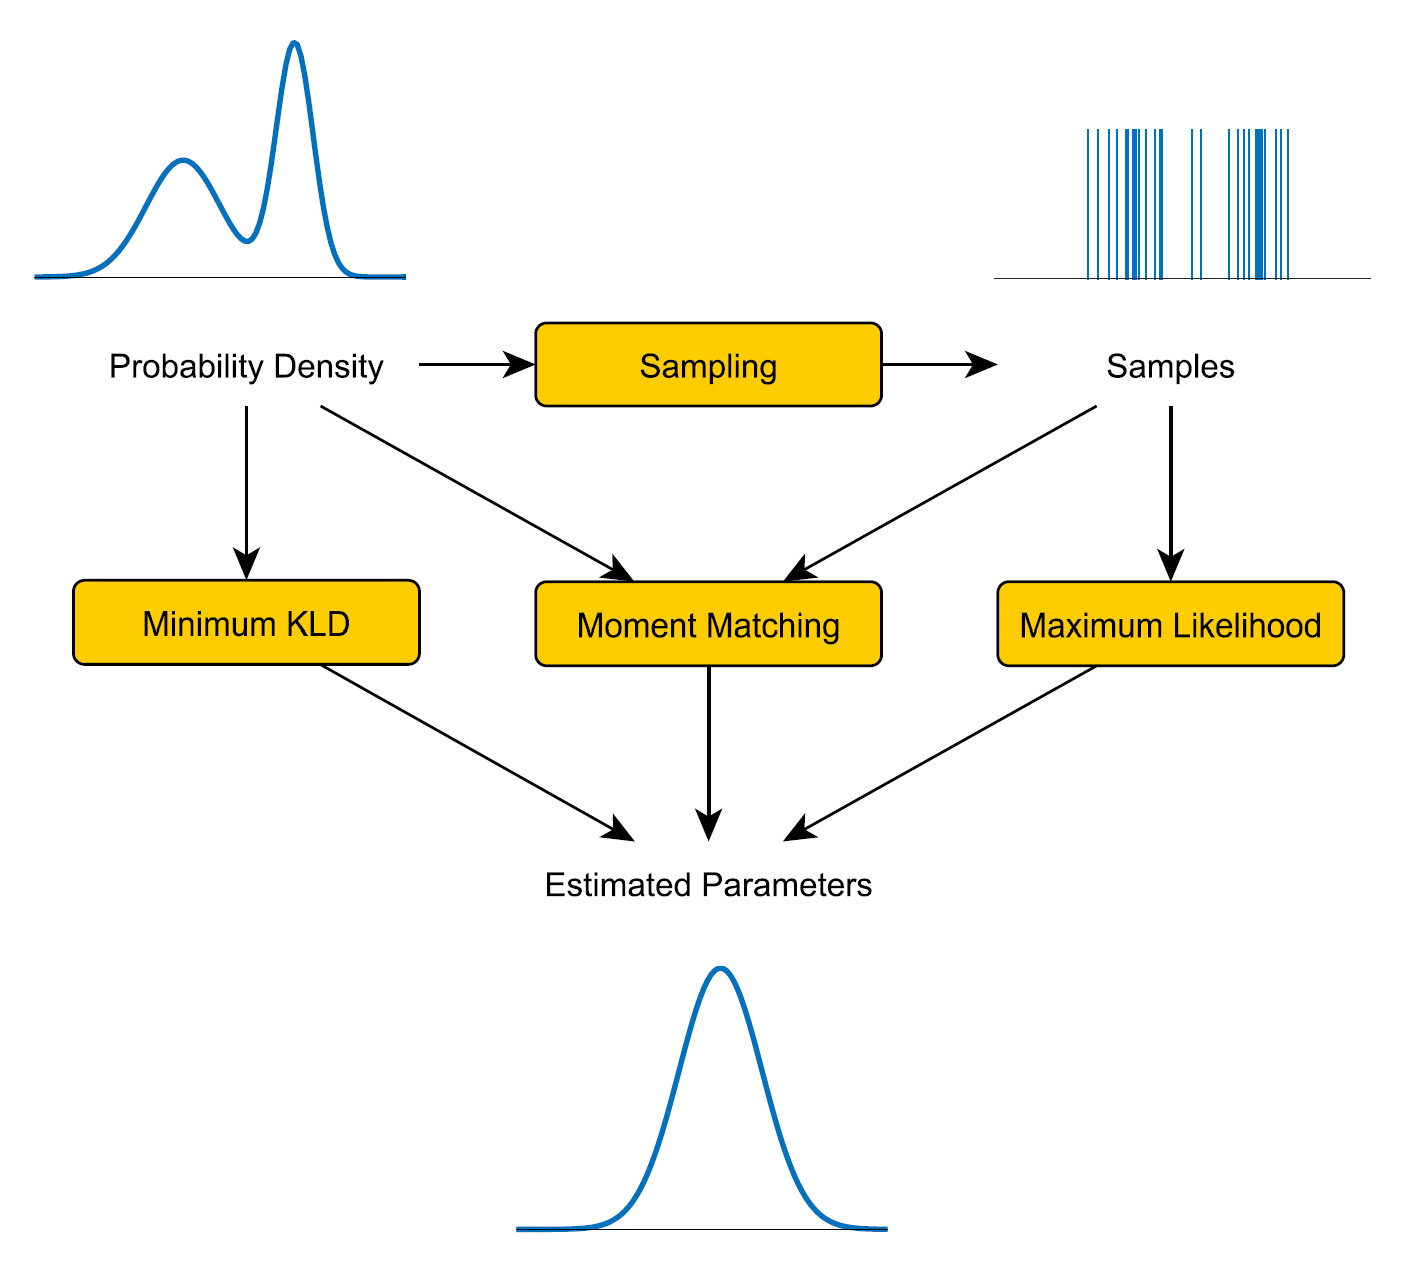
\includegraphics[width=0.6\textwidth]{fig/moment-matching.png}
    \caption{矩匹配}
    \label{fig:moment-match}
\end{figure}

\subsection{定义}

根据上述理解,物理学中与数学中的矩概念相通,即距离(概率)乘以物理量(随机变量)的大小。$p_i$为概率质量函数(Probability mass function,PMF),则对于n阶矩的离散形式有:
\begin{equation*}
    \E[x^n] = \sum_i x_i^n p_i
\end{equation*}

在连续形式下,n阶矩可以表示为$(x-c)^n$的期望,其中$f(x)$为概率密度函数(Probability density function,PDF),其中c为均值。当c为0时,即称为中心距(Central moment)。相反,则称为非中心矩,或原始矩(Raw moment):
\begin{equation*}
    \E[x^n] = \mu_n = \int_{-\infty}^{\infty} (x-c)^n f(x) dx
\end{equation*}

除了根据$c$是否为零,根据是否进行标准化处理,可细分为标准矩。常用的矩有:
\begin{itemize}
    \item 均值 $\text{Mean}(X)=\E(X)$ 为一阶非中心矩
    \item 方差 $\text{Variance}(X) = \E(X-\mu)^2$ 为二阶中心矩
    \item 偏度 $\text{Skewness}(X) = \frac{\E[(X-\mu)^4]}{\sigma^3}$ 为三阶标准矩 
    \item 峰度 $\text{Kurtosis}(X) = \frac{\E[(X-\mu)^4]}{\sigma^4}$ 为四阶标准矩
\end{itemize}

\subsection{分类}

根据如上定义,从零阶至四阶的原始矩与中心矩有如下定义,其中定义$\sigma = \left(\E\left[(X-\mu)^2\right]\right)^{\frac{1}{2}}$。正态分布由它的前两阶矩决定,而对于其他的分布,需要了解更高阶矩。同时注意到三阶矩以上都称标准矩,如同方差要去除均值的影响,偏度和峰度也要去除方差的影响。
\begin{table}[H]
\centering
\begin{tabular}{@{}clll@{}}
\toprule
\textbf{阶} & \multicolumn{1}{c}{\textbf{原始矩}} & \multicolumn{1}{c}{\textbf{中心矩}} & \multicolumn{1}{c}{\textbf{标准矩}} \\ \midrule
\textbf{0} & $\E(x^0)= 1 $ & $\E[(X-\mu)^0] = 1$ & $\frac{\E[(X-\mu)^0]}{\sigma^0} = 1$ \\
\textbf{1} & $\E(x^1)= \mu \,\text{(均值)} $ & $\E[(X-\mu)^1] = 0$ & $\frac{\E[(X-\mu)^1]}{\sigma^1} = 0$ \\
\textbf{2} & $\E(x^2) $ & $\E[(X-\mu)^2] = \sigma^2$ \,\text{(方差)} & $\frac{\E[(X-\mu)^2]}{\sigma^2} = 1$ \\
\textbf{3} & $\E(x^3) $ & $\E[(X-\mu)^3]$ & $\frac{\E[(X-\mu)^3]}{\sigma^3}\,\text{(偏度)} $ \\
\textbf{4} & $\E(x^4) $ & $\E[(X-\mu)^4]$ & $\frac{\E[(X-\mu)^4]}{\sigma^4}\,\text{(峰度)} $ \\ \bottomrule
\end{tabular}
\end{table}

\subsubsection*{原始矩(Raw/crude moment)}

当$c=0$时,称为原始矩。此时则有\textbf{平均数(mean)}或\textbf{期望(expected value)}的连续形式为:
\begin{equation*}
    \E(X) = \mu = \int_{-\infty}^{\infty} (x-0)^1 f(x) dx =
    \int_{-\infty}^{\infty} x f(x) dx
\end{equation*}

其离散形式为:
\begin{equation*}
    \mu = \E(X) = \sum_i x_i p_i
\end{equation*}

\subsubsection*{中心矩(Central moment)}

期望值可以成为随机变量的中心,即当$c=\E(X)$时
\begin{equation*}
    \mu_n = \E[(x-\E(X))^n] = \int_{-\infty}^{\infty} \left(x-\E(X)\right)^n f(x) dx
\end{equation*}

同时可知任何变量的一阶中心矩为0:
\begin{align*}
    \mu_1 &= \int_{-\infty}^{\infty} \left(x-\E(X)\right)^1 f(x) dx \\
    &= \int_{-\infty}^{\infty} x f(x) dx - \int_{-\infty}^{\infty} \E(X) f(x) dx \\
    &= \E(X) - \E(X) \int_{-\infty}^{\infty} f(x) dx \\
    &= \E(X) - \E(X) \times 1 = 0 
\end{align*}

而二阶中心矩(second central moment)为\textbf{方差(Variance)}
\begin{align*}
    \mu_2 &= \int_{-\infty}^{\infty} \left(x-\E(X)\right)^2 f(x) dx \\
    &= \int_{-\infty}^{\infty} x^2 f(x)dx - 2 \E(X) \int_{-\infty}^{\infty} x f(x)dx + \E^2(X)\int_{-\infty}^{\infty}f(x)dx \\
    &= \int_{-\infty}^{\infty} x^2 f(x)dx - 2 \E(X) \E(X) + \E^2(X)\times 1 \\
    &= \int_{-\infty}^{\infty} x^2 f(x)dx - \E^2(X) \\
    &= \E(X^2) - \E^2(X) = \sigma^2
\end{align*}

其离散形式则有:
\begin{equation*}
    \text{Var}(X) = \sigma^2 = \sum p_i (x_i - \E(X))^2 
\end{equation*}

\subsubsection*{标准矩(Standardized moment)}

标准矩为标准化(除以标准差)后的中心矩,第$n$阶中心矩(standardized moment of degree n)有:
\begin{equation*}
    \mu_n = \E[(X-\mu)^n] = \int_{-\infty}^{\infty} (x-\mu)^n f(x)dx
\end{equation*}

已知标准差的$n$次方有:
\begin{equation*}
    \sigma^n = \left(\sqrt{\E[(X-\mu)^2]}\right)^n = \left( \E \left[ (X-\mu)^2\right]\right)^{\frac{n}{2}}
\end{equation*}

此时,第$n$阶标准矩有:
\begin{equation*}
    \wt{\mu}_n = \frac{\mu_n}{\sigma^n} = \frac{\E\left[(X-\mu)^n\right]}{\sigma^n}
\end{equation*}

由一阶中心矩为$0$,可知一阶标准矩(first standardized moment)也为$0$。而二阶标准矩(second standardized moment)则有:
\begin{equation*}
    \wt{\mu}_2 = \frac{\mu_2}{\sigma^2} = \frac{\E[(X-\mu)^2]}{\left(\E[(X-\mu)^2]\right)^{2/2}} = 1
\end{equation*}

\subsubsection*{偏度(skewness)}

三阶标准矩(third standardized moment)为\textbf{偏度}:
\begin{equation*}
    \wt{\mu}_3 = \frac{\mu_3}{\sigma^3} = \frac{\E[(X-\mu)^3]}{\left(\E[(X-\mu)^2]\right)^{3/2}}
\end{equation*}

偏度分为两种:
\begin{itemize}
    \item 负偏态或左偏态:左侧的尾部更长,分布的主体集中在右侧
    \item 正偏态或右偏态:右侧的尾部更长,分布的主体集中在左侧
\end{itemize}

\begin{figure}[H]
    \centering
    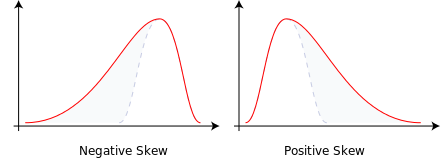
\includegraphics[width=0.8\textwidth]{fig/skewness.png}
    \caption{偏度}
    \label{fig:skew}
\end{figure}

\subsubsection*{峰度(kurtosis)}
四阶标准矩(third standardized moment)为\textbf{峰度}:
\begin{equation*}
    \wt{\mu}_4 = \frac{\mu_4}{\sigma^4} = \frac{\E[(X-\mu)^4]}{\left(\E[(X-\mu)^2]\right)^{4/2}} 
\end{equation*}

由于正态分布的峰度$K(X)=3$,因此定义\textbf{超额峰度(Excess kurtosis)}为峰度$K(X)-3$,那么就有正态分布的超额峰度为$0$:
\begin{equation*}
    \text{Excess kurtosis} = \wt{\mu}_4-3
\end{equation*}
\begin{itemize}
    \item 若超额峰度为正,称为高狭峰(Leptokurtic),此时有尖峰厚尾。即相比正态分布,其“质量”更集中于中心
    \item 若超额峰度为负,称为低阔峰(Platykurtic),此时有低峰轻尾。相比于正态分布,其“质量”在中心位置更分散
\end{itemize}

\begin{figure}[H]
    \centering
    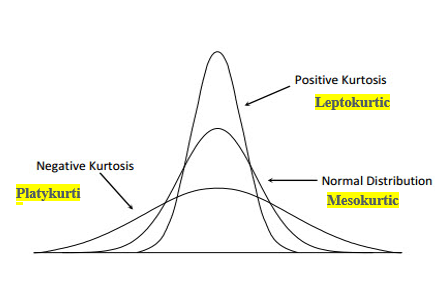
\includegraphics[width=0.7\textwidth]{fig/kurtosis.png}
    \caption{峰度}
    \label{fig:kurt}
\end{figure}

\subsection{矩母函数}

\subsubsection{定义}

矩母函数或称为矩生成函数(Moment generating fuction,MGF)或动差生成函数,顾名思义就是产生矩的函数。对于随机变量$X$,其矩生成函数定义为:
\begin{equation*}
    \boxed{
        M_X(t) = \E(e^{tX})
    }
\end{equation*}

离散形式下有:
\begin{equation*}
    \E[e^{tX}] = \sum e^{tx} p(x)
\end{equation*}

而在连续形势下有:
\begin{equation*}
    \E[e^{tX}] = \int_{-\infty}^{\infty} e^{tx} f(x) dx
\end{equation*}

\begin{thm}
    将矩母函数进行n次求导,并令$t=0$则可得到$\E(X^n)$
    \begin{equation*}
        \E(X^n) = \left. \frac{d^n}{dt^n} M_X(t) \right\vert_{t=0}
    \end{equation*}
\end{thm}

\begin{proof}
    对于$e^x$使用泰勒展开有:
    \begin{equation*}
        e^x = 1 + x + \frac{x^2}{2!} + \frac{x^3}{3!} + \dots + \frac{x^n}{n!}
    \end{equation*}

    那么$e^{tx}$的期望为:
    \begin{align*}
        \E[e^{tX}] &= \E\left[1 + tx + \frac{(tx)^2}{2!} + \frac{(tx)^3}{3!} + \dots + \frac{(tx)^n}{n!} \right] \\
        &= \E(1) + t\E(x) + \frac{t^2}{2!}\E(x^2) + \frac{t^3}{3!}\E(x^3) + \dots + \frac{t^n}{n!}\E(x^n) 
    \end{align*}

    对其求一阶导:
    \begin{align*}
        \frac{d}{dt} \E[e^{tX}] 
        &= \frac{d}{dt} \left[ \E(1) + t\E(x) + \frac{t^2}{2!}\E(x^2) + \frac{t^3}{3!}\E(x^3) + \dots + \frac{t^n}{n!}\E(x^n) \right] \\
        &= 0 + \E(x) + t\E(x^2) + \frac{t^2}{2}\E(x^3) + \dots + \frac{t^{n-1}}{(n-1)!}\E(x^n) \\
        & \qquad \text{(代入$t=0$)} \\
        &= 0 + \E(x) + 0 + 0 + \dots + 0 \\
        &= \E(x) 
    \end{align*}
\end{proof}

\subsubsection{性质}

对于标准正态分布$N\sim(0,1)$的矩母函数,则有:
\begin{align*}
    M_X(t) &= \E (e^{tX}) = \int e^{tx} \frac{1}{\sqrt{\pi}} e^{-\frac{1}{2}x^2}dx \\
    &= \int \frac{1}{\sqrt{\pi}} e^{tx-\frac{1}{2}x^2}dx \\
    &= \int \frac{1}{\sqrt{\pi}} e^{-\frac{1}{2} (x^2 -2xt + t^2 -t^2)}dx \\
    &= \int \frac{1}{\sqrt{\pi}} e^{-\frac{1}{2} (x-t)^2 + \frac{1}{2}t^2}dx \\
    &= e^{\frac{1}{2} t^2} \int \frac{1}{\sqrt{\pi}} e^{-\frac{1}{2} (x-t)^2 }dx \\
    &= e^{\frac{1}{2} t^2}
\end{align*}

对于正态分布$N\sim(\mu,\sigma)$的矩母函数,则有:
\begin{equation*}
    M_X(t) = \E (e^{xt}) = \int e^{xt} \frac{1}{\sigma\sqrt{\pi}} e^{-\frac{1}{2} \left( \frac{X-\mu}{\sigma} \right)} dx
\end{equation*}

此时代换$z=\frac{X-\mu}{\sigma}$,即$x= \sigma z + \mu$,并有$dx=\sigma dz$:
\begin{align*}
    M_X(t) &= \int e^{(\sigma z + \mu)t} \frac{1}{\sigma\sqrt{\pi}} e^{-\frac{1}{2}z^2}dx \\
    &= e^{\mu t} \int e^{\sigma z t} \frac{1}{\sigma\sqrt{\pi}} e^{-\frac{1}{2}z^2}dx \\
    &= e^{\mu t} \int \frac{1}{\sigma\sqrt{\pi}} e^{-\frac{1}{2} (z^2 -2\sigma t z + (\sigma t)^2 -(\sigma t)^2)}dx \\
    &= e^{\mu t} e^{\frac{1}{2} \sigma^2 t^2} \int \frac{1}{\sigma\sqrt{\pi}} e^{-\frac{1}{2} (z - \sigma t)^2}dx \\
    &= e^{\mu t + \frac{1}{2} \sigma^2 t^2}
\end{align*}

\section{假设检验}

\subsection{整体思想}

在假设检验(Statistical hypothesis testing)中,\textbf{原假设}(Null hypothesis,$H_0$),也称为零假设或虚无假设。而与原假设相反的假设称为\textbf{备择假设}(Althernative hypothesis,$H_a$)。假设检验的核心为\textbf{反证法}。在数学中,由于不能穷举所有可能性,因此无法通过举例的方式证明一个命题的正确性。但是可以通过举一个反例,来证明命题的错误。在掷骰子的例子中,在每次掷的过程相当于一次举例,假设进行了上万次的实验,即便实验结果均值为3.5,也无法证明总体的均值为3.5,因为无法穷举。

可以理解为原假设为希望拒绝的假设,或反证法中希望推翻的命题。我们先构造一个小概率事件作为原假设($\text{H}_0$),并假设其正确。如样本均值等于某值,两个样本均值是否相等,样本中的不同组直接是否等概率发生,一般使用等式(小概率)作为原假设。如果抽样检验中小概率事件发生,则说明原假设的正确性值得怀疑。如此时假设实验的结果(样本)远大于或小于理论计算结果3.5,即发生了小概率事件,那么就有理由相信举出了一个反例,这时就可以否定原命题(reject the null hypothesis)。而相反,如果原假设认为均值为3.5,在实验的过程中结果大概率不会偏离这个理论值太多,可以认为我们并没办法举出反例。由于不能直接证明原命题为真,只能说”We can not(fail to) reject the null hypothesis“,无法拒绝原命题。

在需要评估总体数据的时候,由于经常无法统计全部数据,需要从总体中抽出一部分样本进行评估。假设掷骰子一个骰子,其期望为3.5,但假设掷骰子了100次,计算均值为3.47,由于总体的理论值和样本呢的实验值可能存在偏差,误差永远存在,无法避免。那么是否可以认为么3.47“等于”3.5?这时候就需要要界定一个\textbf{显著水平}(Significant level,$\alpha$),相当于设定一个等于的阈值范围。即多小概率的事情发生,是$10\%$还是$5\%$的概率,使我们认为举出了一个反例,值得去怀疑原命题的正确性。当我们知道随机变量的分布时候,根据所进行的检验,我们可以根据计算出的\textbf{统计量}(Test statistic),由于分布已知,统计量对应了一个\textbf{p值}(p-value),即小概率(极端)事件发生的概率,因此在图形上表示为统计量向两侧延申的线下区域。如果这个概率足够低,如小于$\alpha=5\%$,那么就有理由拒绝原假设。

用1-显著水平($1-\alpha$),得到值称为\textbf{置信水平}(Confidence level)(概率大小)。置信水平越大,对应的置信区间也越大(随机变量范围)。此时有置信水平为$1-\alpha$,假设置信区间为$(a,b)$,对于随机变量$x$有$P(a<x<b)=1-\alpha$。对于双侧检验,有置信水平为$1-\alpha$(概率大小),两侧拒绝域分别为$\alpha/2$。对于单侧检验,则有单侧拒绝域大小为$\alpha$。

\subsection{参数与非参数检验}

\textbf{参数检验}(Parametric test)指总体分布服从正态分布或总体分布已知的情况下的统计检验,如z检验、t检验、方差分析(ANOVA)等。单因素方差分析(One-way ANOVA)是检验由单一因素影响的两组样本均值是否存在显著差异,同时有双因素方差分析(Two-way ANOVA)或多因素方差分析(Multi-way ANOVA),单因素与多因素是对于自变量(或称为因子)而言的,两者都是检验对于单因变量或单变量(Univariate)的影响。如上所述,若因变量只有一个,称为单变量方差分析。而多变量方差分析(Multivariate analysis of variance,MANOVA),指当因变量为两个或两个以上的情形。

\textbf{非参数检验}(Nonparametric test)指总体分布不要求服从正态分布或总体分布情况不明时(未知分布、样本太少),用来检验数据是否来自同一个总体的统计检验方法。如卡方检验(Chi-squared test,$\chi^2$ test),其中最著名的为皮尔逊卡方检验(Pearson's $\chi^2$),其他的卡方检验还有如费希尔精确检验(Fisher's exact test)二项检验(Binomial test)。其他的非参数检验还有曼-惠特尼U检验(Mann-Whitney U-test)、K-S检验(Kolmogorov-Smirnov test)、K-W检验(Kruskal-Wallis test)等等。

\subsection{标准差与标准误}
    
\uline{标准差}与\uline{标准误}都衡量的是离散程度,区别在于两者衡量离散程度的对象不同。标准差衡量的对象为一次抽样里样本个体(样本量为$n$)间的离散程度。而标准误衡量的对象,为从同一总体多次抽样得到的多个样本(每个样本量为$n$),每个的样本的某种\uline{统计量}(均值、标准差、中位数,分位数等等),为该统计量的标准差。因此当统计量为样本均值时,此时样本均值标准误(Standard error of the mean,SEM)衡量的为样本均值的离散程度。

假设$X_1,X_2,\dots,X_n$为n个独立观察值,并且有总体均值为$\mu$,总体标准差为$\sigma$,此时对于样本均值的方差有:
\begin{align*}
    \Var(\bar{X}) &= \Var\left(\frac{X_1 + X_2 + \dots + X_n}{n}\right) \\
    &= \frac{1}{n^2} \Var\left(X_1 + X_2 + \dots + X_n\right) \\
    &= \frac{1}{n^2} \left[ \Var(X_1) + \Var(X_2) + \dots + \Var(X_n) \right] \\
    &= \frac{1}{n^2} [n\sigma^2] \\
    &= \frac{\sigma^2}{n}
\end{align*}

可以发现样本均值服从$\bar{X}\sim N(\mu,\frac{\sigma^2}{n})$的正态分布,分母$n$可以理解为对样本容量的调整。此时标准误$s.e.(\bar{X})$,具体而言即样本均值的标准差(Standard deviation of the sample means),下文使用$s.d.(\bar{X})$或$\sigma_{\bar{X}}$表示,由样本均值的方差开方得到。若总体标准差未知,当样本容量30时,样本标准差趋近于总体标准差,使用样本标准差$\hat{\sigma}$代替。
\begin{equation*}
    s.e(\bar{X}) = \frac{\sigma}{\sqrt{n}}
\end{equation*}

对于样本均值的标准误可以用如上简单公式计算得到,当样本量太小、正态分布假设不满足,或没有简单公式可以计算标准误时,可以采用\uline{自助法}(Bootstrapping)重抽样的方法模拟出一个抽样分布。具体而言,对于一个样本量为$n$的样本,重复进行多次有放回的随机抽样,每次抽样时,样本量也均为$n$。注意此时为有放回的抽样,因此样本中的个体可能被抽样多次。对每次抽样都计算所关注的统计量(如均值),从而可以直接获得一个关于该统计量的抽样分布。

【待核实】
当检验的为统计量时,如均值,则分母使用标准误(对应统计量的标准差):
\begin{equation*}
    \frac{\bar{X} - X'}{s.e.(\bar{X})} \quad\text{或}\quad \frac{\bar{X} - X'}{s.d.(\bar{X})}
\end{equation*}

当检验的为样本中的单个观察值时,则使用标准差:
\begin{equation*}
    \frac{X_i - X'}{s.d.(X)}
\end{equation*}

\subsection{Z检验}

Z检验(Z-test)是一种参数检验,用于当\uline{总体均值与标准差已知},或样本量大于30时,检验样本均值与总体均值是否有显著差异。z统计量(z-statistic)服从正态分布(查表用z-table):
\begin{equation*}
    z\text{-statistic} = \frac{\bar{X}-\mu}{s.d.(\bar{X})} = \frac{\bar{X} - \mu}{\sigma/\sqrt{n}}
\end{equation*}

\begin{figure}[H]
    \centering
    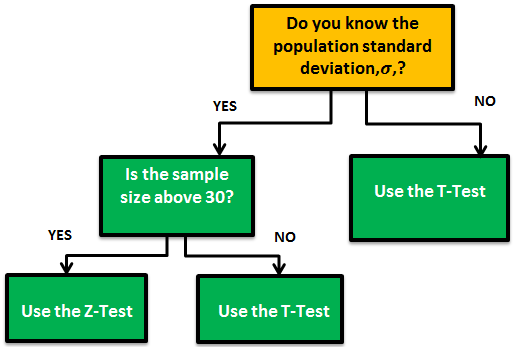
\includegraphics[width=0.6\textwidth]{fig/z-vs-t-test.png}
    \caption{Z-test与T-test}
    \label{fig:z-vs-t-test}
\end{figure}

\subsection{T检验}

T检验(或称Student's t test)是一种参数检验,即假设样本服从或近似服从正态分布。用于样本较小(样本量小于30)或\uline{总体标准差未知}的情形。有如下常见的四个用途:
\begin{itemize}
    \item 单样本均值检验(One-sample t-test):用于检验\uline{单样本的均值}是否与已知的\uline{总体均值}相等
    \item 回归系数的显著性检验(t-test for regression coefficient significance):用于检验\uline{回归模型的解释变量对被解释变量是否有显著影响}
    \item 两独立样本均值检验(Independent two-sample t-test):用于检验\uline{两对独立}的正态或近似正态的\uline{样本的均值}是否相等,这里可根据总体方差是否相等分类讨论
    \item 配对样本均值检验(Dependent t-test for paired samples):用于检验\uline{一对配对样本均值的差}是否等于某一个值
\end{itemize}

\subsubsection{单样本检验}

对于检验单样本样本均值与总体均值是否有差异(One-sample t-test),t统计量(t-statistics)服从t-分布(查表用t-table,单样本自由度为$n-1$,$n$为样本数量),基于样本标准差。t-分布描述了的是标准化(Standardized)的样本均值$\bar{X}$与总体均值$\mu$的距离,即t统计量描述了此时\uline{样本均值距离总体均值多少个标准差}。其中分母为样本标准误(Standard error)为$\sigma/\sqrt{n}$,$\hat{\sigma}$为样本标准差。因此有:
\begin{equation*}
    t\text{-statistic} = \frac{\bar{X}-\mu}{s.e.(\bar{X})} = \frac{\bar{X}-\mu}{\hat{\sigma}/\sqrt{n}}
\end{equation*}

如下所示为t-分布的概率密度函数(PDF),其中$\nu=n-1$为自由度,$\Gamma$为Gamma函数(Gamma function):
\begin{equation*}
    f(t) = \frac{\Gamma\left( \frac{\nu+1}{2} \right)}{\sqrt{\nu\pi} \Gamma\left( \frac{\nu}{2} \right)} \left( 1+\frac{t^2}{\nu} \right)^{-\frac{\nu+1}{2}}
\end{equation*}

而z分布与t分布的差异可见图\ref{fig:z-and-t-dist},并且根据自由度不同而不同,以下图为例,可以看到当自由度变大,当样本量$n$变大时t分布不断接近标准正态分布。z分布与t分布两者都有均值为$0$。
\begin{figure}[H]
    \centering
    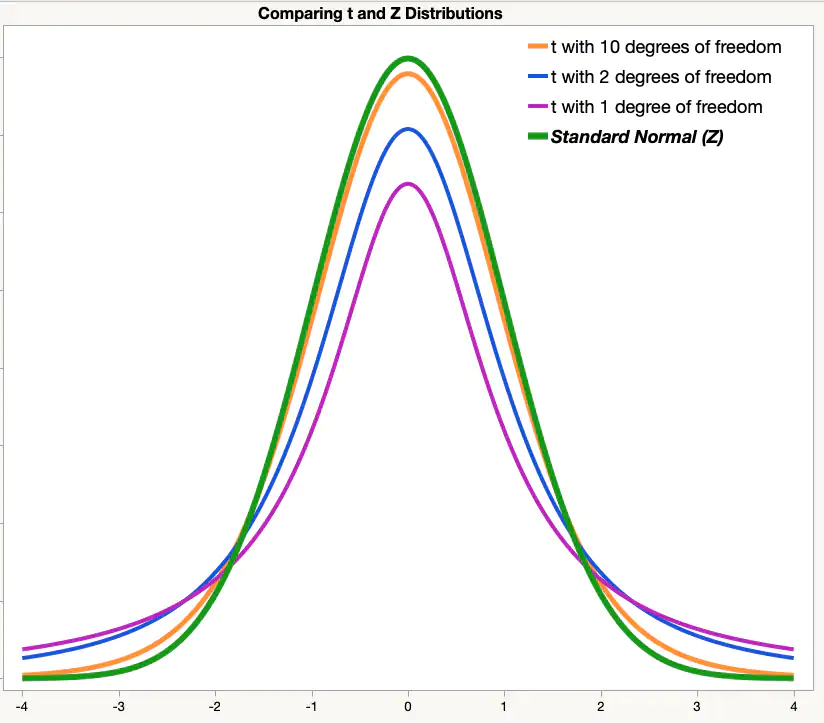
\includegraphics[width=0.6\textwidth]{fig/z-dist-and-t-dist.png}
    \caption{z分布与t分布的差异}
    \label{fig:z-and-t-dist}
\end{figure}

\subsubsection{两独立样本}

检验两个正态总体均值是否相等(Independent two-sample t-test)

【待补充】

\subsubsection{一元回归系数检验}

假设有如下总体回归模型,$X$已知,$\beta_0$与$\beta_1$为待估参数,且$\varepsilon$服从均值为0,方差未知假设为$\sigma^2$的正态分布:
\begin{equation*}
    Y_i = \beta_0 + \beta_1 X_i + \varepsilon_i
\end{equation*}

同时有样本回归模型:
\begin{equation*}
    Y_i = \hat{\beta}_0 + \hat{\beta}_1 X + e_i
\end{equation*}

此时检验回归系数估计值$\hat{\beta}_1$是否等于某$\beta'$,一般假设$\beta' = 0$,即原假设为$X$与$Y$两者不存在线性关系。t-统计量(t-statistic或t-score)服从自由度为$n-2$的t分布:
\begin{equation*}
    t\text{-statistic} = \frac{\hat{\beta}_1 - \beta'}{s.e.(\hat{\beta}_1)} \sim T_{n-2}
\end{equation*}

其中有$\hat{\beta}_1$的标准误,即统计量$\hat{\beta}_1$的标准差,当总体方差已知时:
\begin{equation*}
    s.e.(\hat{\beta}_1) = \frac{\sigma}{\sqrt{\sum_{i=1}^{n} (X_i - \bar{X})^2}}
\end{equation*}

当总体方差未知时,对于$\sigma^2$的无偏估计量$\hat{\sigma}^2$,即为均方残差(Mean squared error)有:
\begin{equation*}
    \hat{\sigma}^2 = \frac{\text{SSE}}{n-2} = \text{MSE}
\end{equation*}

那么此时:
\begin{align*}
    s.e.(\hat{\beta}_1) &= \frac{\hat{\sigma}}{\sqrt{\sum_{i=1}^{n} (X_i - \bar{X})^2}} \\
    &= \frac{\sqrt{\text{SSE}/(n-2)}}{\sqrt{\sum_{i=1}^{n} (X_i - \bar{X})^2}} \\
    &= \frac{\sqrt{\sum_{i=1}^{n} (Y_i - \hat{Y}_i)^2 / (n-2)}}{\sqrt{\sum_{i=1}^{n} (X_i - \bar{X})^2}}
\end{align*}

\subsubsection{多元线性回归系数}

检验在多元线性回归中,$x_1,x_2,\dots,x_m$是否存在线性关系:

\begin{equation*}
    H_0: \beta_i = 0, \quad i=1,2,\dots,m
\end{equation*}

【待补充】

\subsection{F检验}

F检验(F-test),即检验统计量(Test statistic)在原假设下服从F分布(F-distribution)

主要的作用有如下三大类,而方差分析有可以分为许多类,如按照因素区分可分为单因素和多因素:
\begin{itemize}
    \item 方差齐性F检验(F-test of equality of variances)
    \item 方差分析(Analysis of Variance, ANOVA)
    \item 线性回归整体显著性检验(F-test of overall significance in regression)
\end{itemize}

具体而言,$S_1$与$S_2$为独立随机变量,且服从$\chi^2$分布(多个独立服从标准正态分布随机变量的平方和),那么自由度为$\nu_1$与$\nu_2$的服从F分布的随机变量$F$为:
\begin{equation*}
    F = \frac{S_1/\nu_1}{S_2/\nu_2}
\end{equation*}

F分布的概率密度函数为,注意有$x\geq 0$,因为其为两个方差的比率:
\begin{equation*}
    F\text{-distribution} = \frac{\Gamma\left(\frac{\nu_1+\nu_2}{2}\right)\left(\frac{\nu_1}{\nu_2}\right)^{\frac{\nu_1}{2}} x^{\frac{\nu_1}{2}-1}}{\Gamma\left(\frac{\nu_1}{2}\right)\Gamma\left(\frac{\nu_2}{2}\right)\left(1+\frac{\nu_1}{\nu_2}x\right)^{\frac{\nu_1+\nu_2}{2}}} \quad \text{for}\; x\geq 0
\end{equation*}

$n$为样本数,$K$为变量数目,F统计量服从以自由度为$\nu_1$与$\nu_2$的F分布(查表用F-table):
\begin{equation*}
    F\text{-statistic} \sim F_{\nu_1,\nu_2}
\end{equation*}

F分布概率密度函数(PDF)如下图所述,为右偏(Right skew)或正偏(Postive skew)。当$\nu_2>2$时,期望有$\frac{\nu_2}{\nu_2 -2}$。
\begin{figure}
\centering
\begin{subfigure}{.5\textwidth}
    \centering
    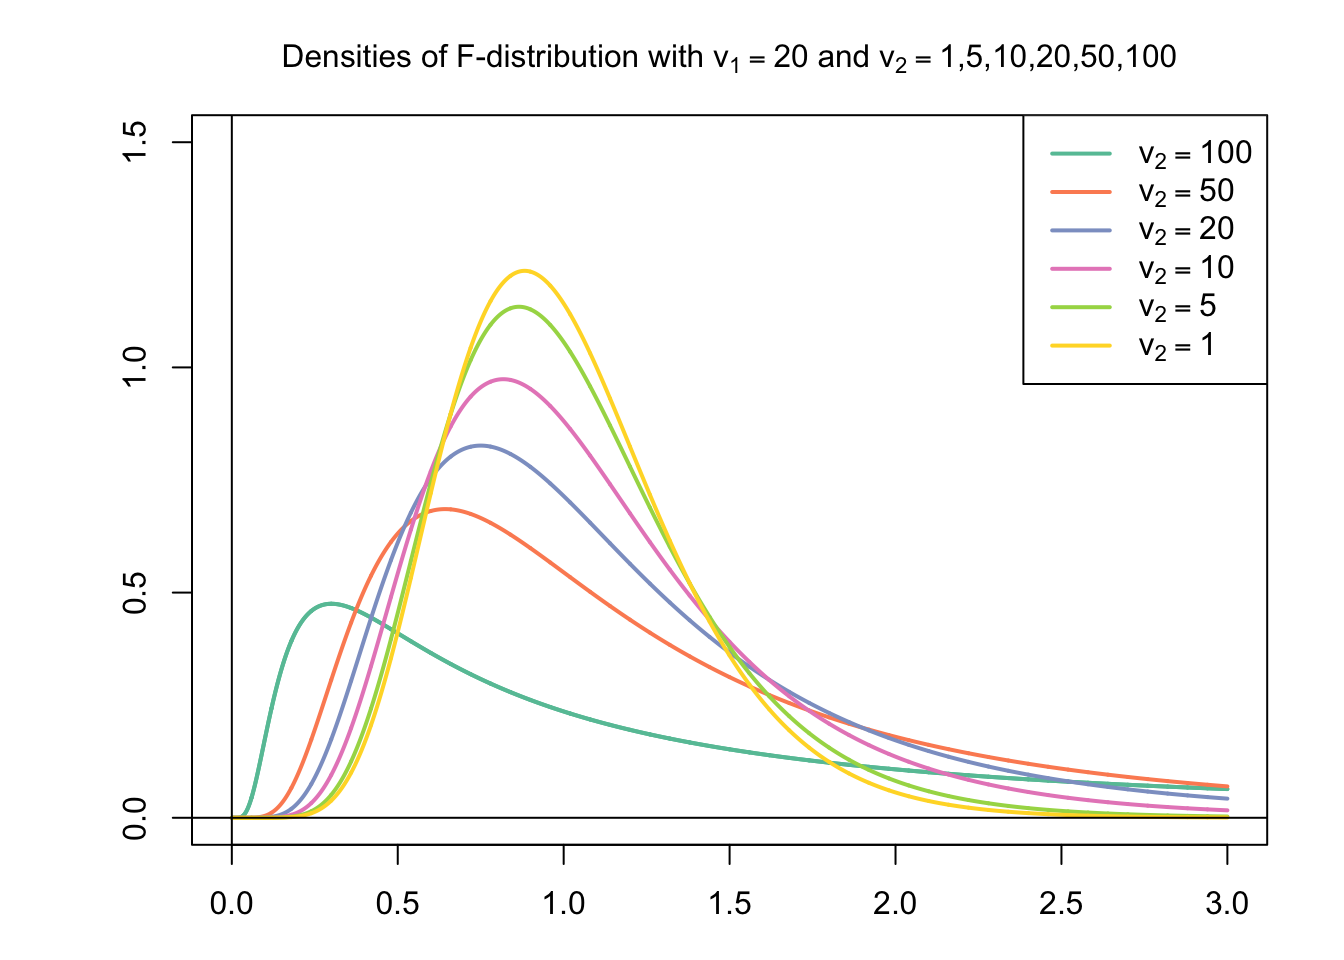
\includegraphics[width=\linewidth]{fig/f-dist-1.png}
    \caption{$\nu_1=20$}
\end{subfigure}%
\begin{subfigure}{.5\textwidth}
    \centering
    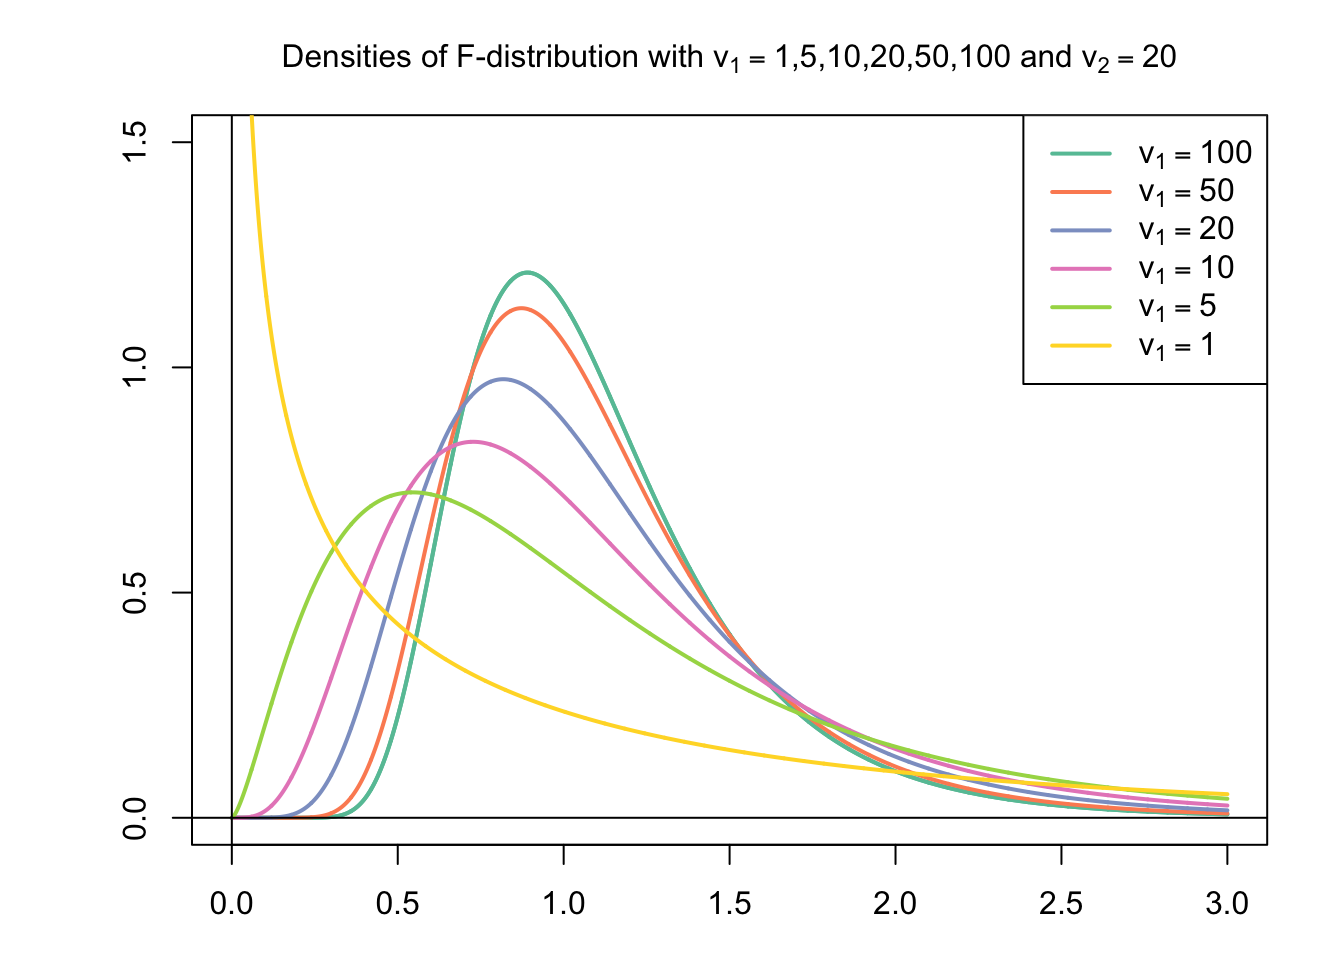
\includegraphics[width=\linewidth]{fig/f-dist-2.png}
    \caption{$\nu_2=20$}
\end{subfigure}
\caption{F分布PDF}
\label{fig:f-dist}
\end{figure}

\subsubsection{方差齐次F检验}

检验两个正态总体之间的方差是否相等,原假设为两个正态分布总体的方差相等。假设$X$与$Y$来自两个独立的服从正态分布的总体,即有$X\sim N(\mu_X^2,\sigma_X^2)$和$Y\sim N(\mu_Y^2,\sigma_Y^2)$,从中抽取$m$与$n$个样本,即$X_1,X_2,\dots,X_m$和$Y_1,Y_2,\dots,Y_n$。

因此两者均值和标准差为:
\begin{gather*}
    \bar{X} = \frac{1}{m} \sum_{i=1}^{m} X_i \qquad 
    S_X^2 = \frac{1}{m-1} \sum_{i=1}^{m} \left(X_i -\bar{X}\right)^2 \\
    \bar{Y} = \frac{1}{n} \sum_{i=1}^{n} Y_i \qquad
    S_Y^2 = \frac{1}{n-1} \sum_{i=1}^{n} \left(Y_i -\bar{Y}\right)^2
\end{gather*}

此时双侧的原假设为假设两总体方差相等,备择假设为假设两总体方差不等:
\begin{align*}
    H_0: \sigma_X^2 = \sigma_Y^2 \\
    H_a: \sigma_Y^2 \neq \sigma_Y^2
\end{align*}

此时F统计量应有,一般约定以较大的方差作为分子,较小的方差作为分母,使得计算出来的$F>1$方便进行查表。假设显著性水平为$\alpha$,此时临界值为$F_{\alpha,(m-1,n-1)}$,当$F>F_{\alpha,(m-1,n-1)}$时,拒绝原假设:
\begin{equation*}
    F = \frac{S_X^2}{S_Y^2} \sim F(m-1,n-1)
\end{equation*}

\subsubsection{方差分析}

方差分析(Analysis of variance,ANOVA),可以用于一次性检验多个(两个或两个以上)总体的均值是否相等,而T检验弱面对多个总体,只能两两进行比较。以单因素方差分析(One-way ANOVA)为例,比较不同组之间的均值是否相同。例如研究不同的猪饲料对猪的增重效果是否不同,此时猪饲料为(单)因素,即不同的配方为不同组(水平),随机取样,观察猪增重效果是否相同。又或研究客户满意程度在不同航空公司之间是否不同,此时航空公司为(单)因素,即不同的航空公司为不同组(水平),随机抽样,观察不同航空公司客户满意度的均值是否相同。
\begin{example}
    航空公司客户满意度(0-10分)例子

    \begin{table}[H]
    \centering
    \begin{tabular}{@{}cccc@{}}
    \toprule
    \textbf{甲航空} & \textbf{乙航空} & \textbf{丙航空} & \textbf{丁航空} \\ \midrule
    8 & 3 & 7 & 8 \\
    6 & 7 & 8 & 9 \\
    7 & 5 & 9 & 6 \\
    5 & 9 &   & 7 \\
    9 &   &   &   \\ \bottomrule
    \end{tabular}
    \end{table}
\end{example}

注意虽然ANOVA叫做方差分析,但是他的目的是检验每个组的均值是否相同。ANOVA的原假设为$K$个总体的均值相等,$H_0: \mu_1 = \mu_2 = \dots = \mu_K$。可以换个角度考虑这个问题,如果几家公司的客户满意度没有显著的差别,那么可以认为是一个总体的四次随机抽样。相反,若有一家航空公司表现与众不同,那么这家航空公司不是来自同一个总体。ANOVA有主要有以下3个假设:
\begin{itemize}
    \item 方差的同质性,可以理解为每组样本背后的总体的的方差相同
    \item 总体遵循正态分布
    \item 每一次抽样都是独立的
\end{itemize}

\textbf{组间}偏差平方和(Sum of square between groups,SSB或SSA)与\textbf{组内}偏差平方和(Sum of square error,SSE)都是偏差的平方和,而两者计算的偏差个数不一样,无法直接相除,因此除以各自的自由度,使得两者在平均的意义下可比。因此有有$MSB = SSB/df_1$和$MSE = SSE/df_2$,其中$df_1=K-1$和$df_2=N-K$为两者自由度。
\begin{equation*}
    F = \frac{SSB/df_1}{SSE/df_2}= \frac{MSB}{MSE} \sim F(K-1,N-K)
\end{equation*}

可以从图\ref{fig:mse-msb}中看到,组内均方(Mean squared error, MSE)对应着为每个样本分布自身的方差。组间均方(Mean squared between,MSB)对应着相当于样本对于总体的方差。可以想象,当两者之间相差越大时,不是来自同一总体(假设)的概率就越大
\begin{figure}[H]
    \centering
    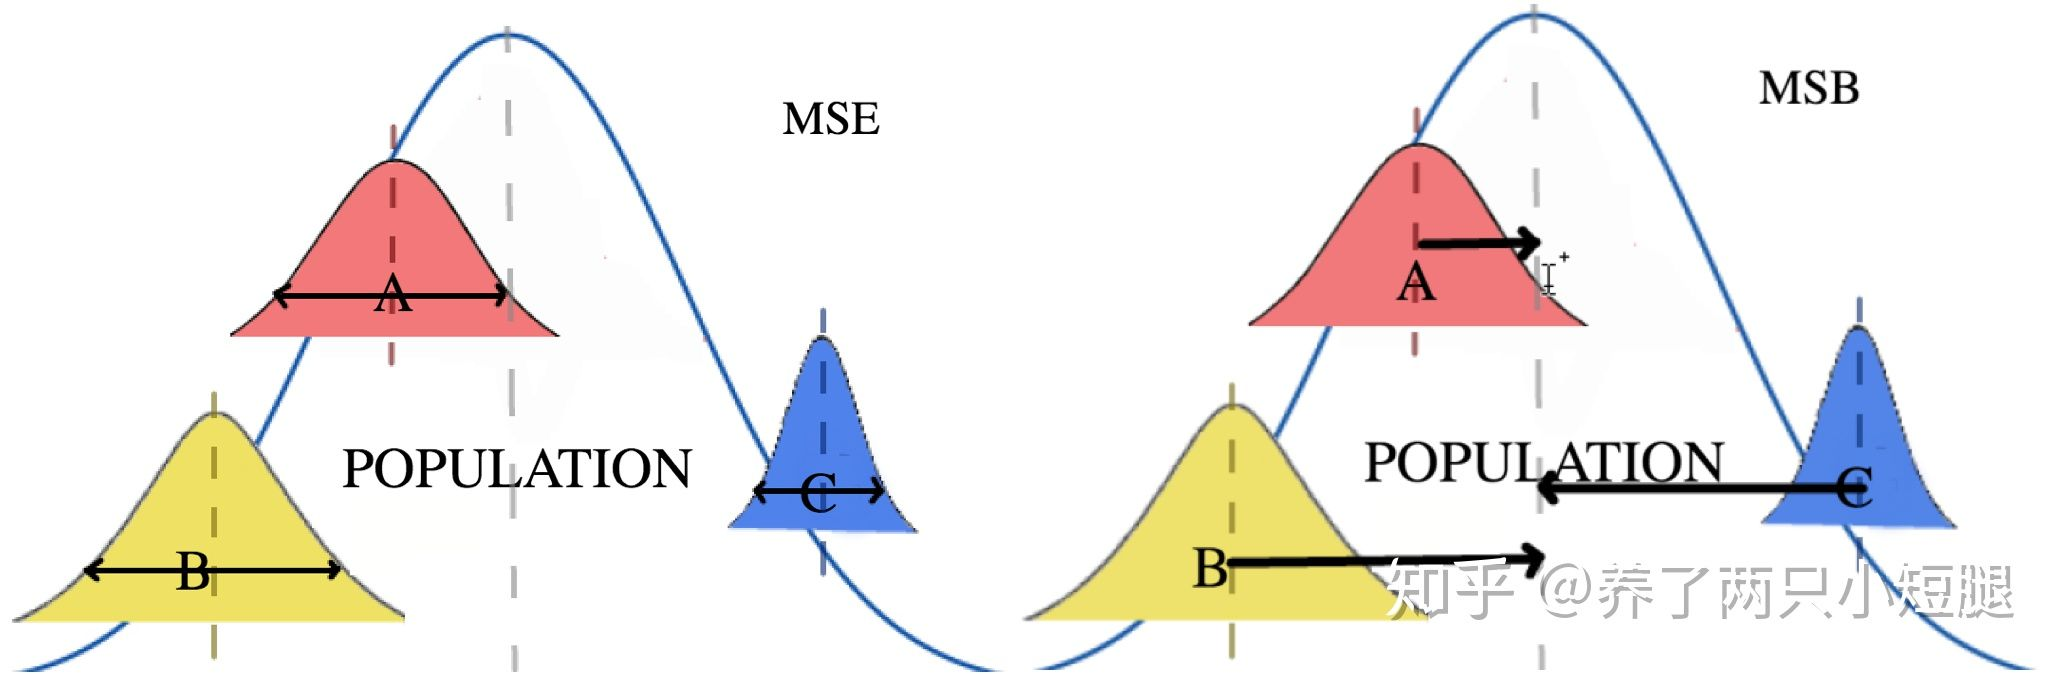
\includegraphics[width=0.8\textwidth]{fig/mse-msb.jpg}
    \caption{MSE和MSB}
    \label{fig:mse-msb}
\end{figure}

方差分析表如下,假设显著性水平为$\alpha$,那么有当$F > F_{\alpha,(K-1,N-K)}$时,可以认为这一次抽样几乎不可能,从而拒绝原假设,认为该因素显著:
\begin{table}[H]
\centering
\begin{tabular}{@{}ccccc@{}}
\toprule
\textbf{偏差来源} & \textbf{偏差平方和} & \textbf{自由度} & \textbf{均方} & \textbf{F值} \\ \midrule
组间 & SSB & $K-1$ & $MSB=\frac{\text{SSB}}{K-1}$ & $\frac{\text{MSA}}{\text{MSE}}$ \\
组内 & SSE & $N-K$ & $MSE=\frac{\text{SSE}}{N-K}$ &                   \\
总计 & SST & $N-1$ &                       &                   \\ \bottomrule
\end{tabular}
\end{table}

具体而言,假设实验共有$K$个分类(水平),总样本量为$N$,每个分类下有$N_i$个体,并有$N=\sum_{i=1}^{K}N_i$,令$x_{i,j}$为第$i$个分类第$j$个样本。

第$i$组的组内均值为:
\begin{equation*}
    \bar{x}_{i,\cdot} = \frac{1}{N_i} \sum_{j=1}^{N_i} x_{i,j}
\end{equation*}

总体均值为:
\begin{equation*}
    \bar{x} = \frac{1}{N} \sum_{i=1}^{K} \sum_{j=1}^{N_i} x_{i,j}
\end{equation*}

因此,组间偏差平方和应为,组均值与总体均值偏差的平方和。一共有$K$组,均值确定后,只有$K-1$可自由变化,因此SSB的自由度为$K-1$:
\begin{equation*}
    SSB = \sum_{i=1}^{K}\sum_{j=1}^{N_i} (\bar{x}_{i,\cdot} - \bar{x})^2 = 
    \sum_{i=1}^{K} N_i ( \bar{x}_{i,\cdot} - \bar{x})^2
\end{equation*}

组内偏差平方和应有,即个体与组内均值偏差的平方和。$N$个个体,每个组的平均值$\bar{x}_{i,\cdot}$确定后,只有$N-K$可自由变动,因此SSE的自由度为$N-K$:
\begin{equation*}
    SSE = \sum_{i=1}^{K}\sum_{j=1}^{N_i} (x_{i,j} - \bar{x}_{i,\cdot})^2
\end{equation*}

那么总偏差平方和(Sum of square total,SST)为个体与总体平均值偏差的平方和。当$\bar{x}$确定后,有$N-1$可自由变换,因此SST自由度为$N-1$:
\begin{equation*}
    SST = \sum_{i=1}^{K}\sum_{j=1}^{N_i} (x_{i,j} - \bar{x})^2 = SSB + SSE
\end{equation*}

\begin{proof}
    对于SST的分解有:
    \begin{align*}
        SST &= \sum_{i=1}^{K}\sum_{j=1}^{N_i} (x_{i,j} - \bar{x})^2 \\
        &= \sum_{i=1}^{K}\sum_{j=1}^{N_i} \left[(x_{i,j} - \bar{x}_{i,\cdot}) + (\bar{x}_{i,\cdot} - \bar{x})\right]^2 \\
        &= \sum_{i=1}^{K}\sum_{j=1}^{N_i} (x_{i,j} - \bar{x}_{i,\cdot})^2 + \sum_{i=1}^{K}\sum_{j=1}^{N_i} (\bar{x}_{i,\cdot} - \bar{x})^2 + 2\sum_{i=1}^{K}\sum_{j=1}^{N_i} (\bar{x}_{i,\cdot} - \bar{x})(x_{i,j} - \bar{x}_{i,\cdot}) \\
        &= \sum_{i=1}^{K}\sum_{j=1}^{N_i} (x_{i,j} - \bar{x}_{i,\cdot})^2 + \sum_{i=1}^{K}\sum_{j=1}^{N_i} (\bar{x}_{i,\cdot} - \bar{x})^2 + 2\sum_{i=1}^{K} \left[ (\bar{x}_{i,\cdot} - \bar{x}) \sum_{j=1}^{N_i} (x_{i,j} - \bar{x}_{i,\cdot}) \right]
    \end{align*}

    由于:
    \begin{equation*}
        \sum_{j=1}^{N_i} (x_{i,j} - \bar{x}_{i,\cdot}) = \sum_{j=1}^{N_i} x_{i,j} - N_i \bar{x}_{i,\cdot} = 0
    \end{equation*}

    因此SST推导中最后一项为0,可以消去,得到最终结果:
    \begin{equation*}
        SST = SSB + SSE
    \end{equation*}
\end{proof}

\subsubsection{线性回归整体显著性检验}

F检验还可以用于检验变量被解释变量$y$与解释变量$x_1,x_2,\dots,x_k$,两者之间的整体线性关系是否显著,检验的是线性方程整体的显著性。假设有如下回归方程:
\begin{equation*}
    y = \beta_0 + \beta_1 x_1 + \beta_2 x_2 + \dots + \beta_k x_k
\end{equation*}

若各回归系数$\beta_i \;(i =1,2,\dots,k)$均为0,则被解释变量$y$与解释变量$x_i\;(i=1,2,\dots,k)$没有任何关系,回归模型变为$y=\beta_0$,只有截距项。反之,若各回归系数$\beta_i$中仅有部分为$0$,则对于这部分回归系数不为0的$x_i$而言,该回归模型还是有意义的。因此原假设与备择假设如下:
\begin{gather*}
    H_0: \beta_1 = \beta_2 = \dots = \beta_k = 0 \\
    H_a: \beta_i (i=1,2,\dots,k) \text{不全为0}
\end{gather*}

方差分析表如下,假设显著性水平为$\alpha$,那么有当$F > F_{\alpha,(p,n-p-1)}$时,可以认为这一次抽样几乎不可能,从而拒绝原假设,认为该因素显著:
\begin{table}[H]
\centering
\begin{tabular}{@{}ccccc@{}}
\toprule
\textbf{偏差来源} & \textbf{偏差平方和} & \textbf{自由度} & \textbf{均方} & \textbf{F值} \\ \midrule
回归 & SSR & $p$ & $MSR=\frac{SSR}{k}$ & $\frac{MSA}{MSE}$ \\
误差 & SSE & $n-p-1$ & $MSE=\frac{SSE}{n-k-1}$ &                   \\
总计 & SST & $n-1$ &                       &                   \\ \bottomrule
\end{tabular}
\end{table}

\subsection{\tops{$\chi^2$}检验}

卡方检验(Chi-squared test)为非参数检验,不存在具体参数和总体正态分布的假设。最初由统计天王Karl Pearson于1900年提出,是三大抽样(T检验、F检验与卡方检验)分布的检验里历史最悠久的。

卡方检验是比较数据的实测(实际观测值)分布与数的预期(理论预期值)分布的假设检验,检验两者之间的偏离程度,实际观测值与理论预期值之间的偏离程度就决定卡方的大小。如果卡方越大,二者偏差程度越大。相反,二者偏差越小。若两个值完全相等时,卡方值就为0,表明理论值完全符合。常见的卡方检验有:
\begin{itemize}
    \item 皮尔逊卡方检验(Pearson's chi squared test)
    \item 耶茨的连续性修正(Yates's correction for continuity)
    \item Fisher确切概率法(Fisher's exact test)
\end{itemize}

假设有随机变量$x_1,x_2,\dots,x_k$为独立随机变量,服从$N(0,1)$的标准正态分布。其令平方和为$Q$,注意此为随机变量的平方和,并非分布的平方和。则有$Q$服从自由度为$k>0$的卡方分布,即:
\begin{equation*}
    Q = \sum_{i=1}^{k} x_i^2 \qquad Q \sim \chi^2(k) \quad\text{or}\quad Q \sim \chi_k^2
\end{equation*}

对于自由度为$k$的卡方分布的概率密度函数(PDF)有:
\begin{equation*}
    f(x) = \frac{1}{2^{\frac{k}{2}}\Gamma\left(\frac{k}{2}\right)} x^{\frac{k}{2}-1} e^{-\frac{x}{2}}
\end{equation*}

卡方检验为单尾检验,拒绝域在右尾。当卡方分布的自由度$k<2$时,曲线呈现倒L形,当$k>2$时趋向于对称,而当$k\rightarrow \infty$时,则趋向于正态分布。
\begin{figure}[H]
    \centering
    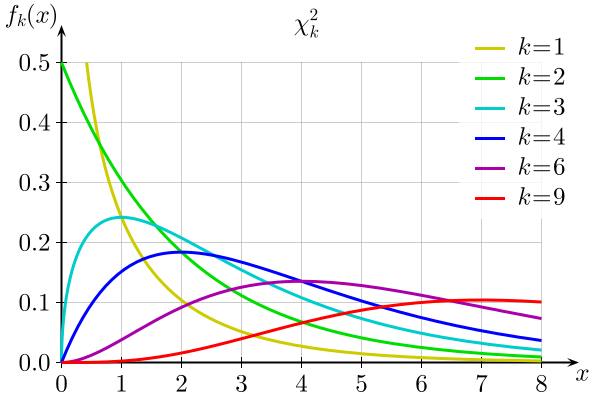
\includegraphics[width=0.8\textwidth]{fig/chi-squared.png}
    \caption{卡方分布PDF}
    \label{fig:chi-squared}
\end{figure}

\subsubsection{皮尔逊卡方检验}

皮尔逊卡方检验(Pearson's chi-squared test),当提及卡方检验,通常即指皮尔逊卡方检验。其中$O_i$指实际观察频数,$E_i$指理论预期频数:
\begin{equation*}
    \chi^2 = \sum_i \frac{(O_i - E_i)^2}{E_i}
\end{equation*}

皮尔逊卡方检验有多种用途:
\begin{itemize}
    \item 卡方拟合优度检验(Chi-square goodness-of-fit tests)
    \begin{itemize}
        \item 用于检验分类数据样本与总体理论分布的拟合程度
        \item 例如,通过多次掷骰子并使用卡方拟合优度检验来确定结果是否服从均匀分布,可以检验骰子是否公平。
    \end{itemize}
    \item 卡方关系检验(Chi-square tests for relationships)
    \begin{itemize}
        \item 独立性检验(Test of independence):可以使用独立性检验确定一个变量的观测值是否取决于另一个变量的观测值。例如,确定总统候选人党派是否与投票人的性别无关(同一人群样本,两个分类变量,性别与党派)。
        \item 同质性检验(Test of homogeneity):可以使用同质性检验不同样本中同一个变量的分布是否相同。例如,确定不同颜色的汽车的销量是否取决于汽车售出的城市(随机选择城市不同样本,汽车颜色为单一变量)
    \end{itemize}
\end{itemize}

\subsubsection*{卡方拟合优度检验}
    
卡方拟合优度检验或称拟合度的卡方检验、最佳拟合度卡方检验,用于检验实际数据是否符合理论分布,即度量实际分布与理论分布的拟合优度(Goodness of fit)。对于离散情形下,假设随机抽样的总样本量为$n$,分为互斥的$k$类,每一类的个体数为$x_i,\; i=1,2,\dots,k$为实际频数(个数),同时有$k$理论频数为,原假设为:
\begin{equation*}
    H_0: \text{第k类的占比为} p_i \quad i=1,2,\dots,k
\end{equation*}

此时有卡方统计量,分子为实际频数与理论频数的平方。服从自由度为$k-1$的卡方分布:
\begin{equation*}
    \chi^2 = \sum_{i=1}^{k} \frac{(x_i-np_i)^2}{np_i} \sim \chi^2(k-1)
\end{equation*}

\begin{example}
    孟德尔提出遗传第二定律,他发现有四种不同种类的豌豆种子:黄色圆形的、黄色褶皱的、绿色圆形的、绿色褶皱的。这些表现型类别(由可观察到的特征定义的类别)以大约9:3:3:1的比例出现。假设实际频数为315:108:101:32,总频数为556。那对于理论频数应有:
    \begin{equation*}
        556 \frac{9}{16} : 556 \frac{3}{16} : 556 \frac{3}{16} : 556 \frac{1}{16} = 312.75:104.25:104.25:34.75
    \end{equation*}

    因此计算卡方统计量有:
    \begin{equation*}
        \chi^2 = \frac{(315-312.75)^2}{312.75} + \frac{(108-104.25)^2}{104.25} + \frac{(101-104.25)^2}{104.25} + \frac{(32-34.75)^2}{34.75} = 0.47
    \end{equation*}

    对于显著性水平$\alpha=0.05$,$\chi_{0.05,3}^2 = 7.815 > 0.47$,因此无法拒绝原假设,实验结果符合理论预期。
\end{example}

\subsubsection*{卡方独立性与同质性检验}

卡方相关性与独立性的检验,检验的方式并无不同,主要差异在于实验的设计和如何解读实验结果。若将不同样本理解为分类变量,也可认为是独立性检验,可以理解为同质性检验为独立性检验的延伸,用于一些特殊情形,例如检验待检测产品的特性、小白鼠的体重等,产品和小白鼠并无实质的差异,当然可以设置为待测产品或小白鼠以不同批次划分,为随机抽取的结果,而非本质上的划分。具体而言,在独立检测中有两个根据其本质划分的分类变量,而在同质性检验中,其中一个变量是随机产生的(随机选取批次),不能视为一个分类变量,因此只能进行同质性检验。
\begin{table}[H]
\centering
\begin{tabular}{@{}ccc@{}}
\toprule
& \textbf{研究对象} & \textbf{研究目的} \\ \midrule
\textbf{独立性} & 单一样本下的两个分类变量 & 同一个样本下,两个分类变量是否独立 \\
\textbf{同质性} & 多个样本下度量同一分类变量 & 不同的样本是否同质,即分类变量的分布是否相同 \\ \bottomrule
\end{tabular}
\end{table}

\begin{example}
    假设在赌场中,老板认为以为负责二十一点的庄家赔付的金额高于平均值,三位庄家观察的数据如下:
    \begin{table}[H]
    \centering
    \begin{tabular}{@{}ccccc@{}}
    \toprule
    & \textbf{庄家甲} & \textbf{庄家乙} & \textbf{庄家丙} & \textbf{合计} \\ \midrule
    \textbf{胜}  & 43 & 49 & 22 & 114 \\
    \textbf{平}  & 8 & 2 & 5 & 15 \\
    \textbf{负}  & 47 & 44 & 30 & 121 \\
    \textbf{合计} & 98 & 95 & 57 & 250 \\ \bottomrule
    \end{tabular}
    \end{table}

    此时原假设为庄家和赌局结果没有关系,即两者独立,而备择假设为有关系,两者不独立。对于庄家甲胜场的情况下,假设庄家与独具相互独立,应有理论频率为:
    \begin{align*}
        P(\text{庄家甲胜场}) &= \text{总场数} \times P(\text{庄家甲参加比例}) \times P(\text{胜场比例}) \\
        &= 250 \times \frac{114}{250} \times \frac{98}{250}
    \end{align*}

    计算所有理论频数为:
    \begin{table}[H]
    \centering
    \begin{tabular}{@{}cccc@{}}
    \toprule
    & \textbf{庄家A}& \textbf{庄家B} & \textbf{庄家C} \\ \midrule
    \textbf{胜} & $(114\times 98)/250$ & $(114\times 95)/250$ & $(114\times 57)/250$ \\
    \textbf{平} & $(15\times 98)/250$  & $(15\times 95)/250$  & $(15\times 57)/250$  \\
    \textbf{负} & $(121\times 98)/250$ & $(121\times 95)250$  & $(121\times 57)/250$ \\ \bottomrule
    \end{tabular}
    \end{table}

    计算卡方统计量:
    \begin{equation*}
        \chi^2 = \sum_i^n \frac{(O_i - E_i)^2}{E_i} = 5.62
    \end{equation*}

    对于显著性水平$\alpha=0.05$,$\chi^2_{0.05,4} = 9.488 > 5.62$,因此无法拒绝原假设,赌局的胜负与庄家没有关系。
\end{example}

\begin{example}
    以泰坦尼克号的生还者与遇难者的数据为例,计算可计算出生还的概率约为$32\%$,因此头等舱乘客的生还的理论概率为$32\%\times 325 \approx 104$,继续计算所有理论频数。得到$\chi^2 = 192.2$,此时自由度有$df=(4-1)(2-1)=3$,因此在显著水平$\alpha=0.05$下临界值$\chi^2_{0.05,3} = 7.815 < 192.2$,因此拒绝四个类别的乘客生还率相同的原假设。
    \begin{table}[H]
    \centering
    \begin{tabular}{@{}cccccc@{}}
    \toprule
    & \textbf{头等舱} & \textbf{二等舱} & \textbf{三等舱} & \textbf{船员} & \textbf{合计} \\ \midrule
    \textbf{生还} & 202 & 118 & 178 & 215 & 713 \\
    \textbf{遇难} & 123 & 167 & 528 & 698 & 1516 \\
    \textbf{合计} & 325 & 285 & 796 & 913 & 2229 \\ \bottomrule
    \end{tabular}
    \end{table}
\end{example}

\section{条件概率}

\subsection{条件概率}

条件概率(Conditional probability)记为$P(A\given B)$,指已知事件B发生的情况下事件A发生的概率,即把原本的样本空间,缩小为只有B发生的样本空间,从中再计算A发生的概率。而联合概率分布(Joint probability distribution)或简称为\textbf{联合分布},表示两个事件同时发生的概率,记为$P(A,B)$或$P(A\cap B)$,其样本空间为原本未缩小的空间。
\begin{equation*}
    P(A \given B) = \frac{P(A \cap B)}{P(B)}
\end{equation*}

\begin{remark}
    同理$P(B\given A) = \frac{P(A \cap B)}{P(A)}$,即有$P(A \cap B) = P(B\given A)P(A) = P(A\given B)P(B)$。易知同时满足AB条件的概率,即为已知满足A条件的子集中,再满足条件B的概率(为条件概率,即其样本空间为缩小后满足条件A的空间)。或满足条件B的子集中,再满足条件A的概率。
\end{remark}

\begin{example}
    假设有两个小碗,分别为甲碗与乙碗,每个小碗中有若干小球,共有蓝色与黄色两种颜色,具体数量如下。
    \begin{table}[H]
    \centering
    \begin{tabular}{cccc}\toprule
    & \textbf{蓝色} & \textbf{黄色} \\ \midrule
    \textbf{甲碗} & 1 & 4  \\
    \textbf{乙碗} & 3 & 2  \\ \bottomrule
    \end{tabular}
    \end{table}

    那么任意选取一个碗,并从中选取一个小球,颜色为蓝色的概率应为$P(\text{蓝色})=\frac{4}{10}$,同时有$P(\text{黄色})=\frac{6}{10}$。若已知取的碗为甲碗,那么选取蓝色小球的概率应为$P(\text{蓝色}\given \text{碗}=\text{甲碗})=\frac{1}{5}$,此时样本空间改变,被限制在了甲碗中,此时称为条件概率。

    若此时任意从两个碗中选取一个小球,小球颜色是蓝色,那么此时该小球是从甲碗中选取的概率为$P(\text{甲碗}\given \text{颜色}=\text{蓝色})=\frac{1}{4}$,注意$P(\text{甲碗}\given \text{蓝色})$与$P(\text{蓝色}\given \text{甲碗})$的概率并不相同。
\end{example}

\begin{example}
    假设某病患被检测出了某癌症阳性,该癌症在人群中的患病率(Prevalence)为$0.1\%$,并且该诊断的正确率为$99\%$。
    \begin{figure}[H]
    \centering
    \begin{tikzpicture}[
    grow = right, 
    level distance = 7em,
    level 1/.style={sibling distance=4.5em, anchor=west},
    level 2/.style={sibling distance=3em, anchor=west},
    ]
    \node {病患}
    child {
        node {不患癌症} 
        child {node {检测阴性} edge from parent node [above,sloped] {0.99}}
        child {node {检测阳性} edge from parent node [above,sloped] {0.01}}
        edge from parent node [above,sloped]{0.999}
    }
    child {
        node {患有癌症} 
        child {node {检测阴性} edge from parent node [above, sloped] {0.01}}
        child {node {检测阳性} edge from parent node [above,sloped] {0.99}}
        edge from parent node [above,sloped]{0.001}
    };
    \end{tikzpicture}
    \end{figure}

    该病人检测为阳性,因此有关的概率为$P(\text{患有癌症} \cap \text{检测阳性})$与$P(\text{不患癌症} \cap \text{检测阳性})$,而该病人在检测为阳性的前提下,真正患有癌症的概率应为:
    \begin{align*}
        P(\text{患有癌症}\given \text{检测阳性}) &= \frac{P(\text{患有癌症} \cap \text{检测阳性})}{P(\text{检测阳性})} \\
        &= \frac{P(\text{患有癌症} \cap \text{检测阳性})}{P(\text{患有癌症} \cap \text{检测阳性}) + P(\text{不患癌症} \cap \text{检测阳性})} \\
        &= \frac{0.001 \times 0.99}{0.001\times 0.99 + 0.999\times 0.01} \approx 9.016\% 
    \end{align*}

    或使用表格表示:
    \begin{table}[H]
    \centering
    \begin{tabular}{@{}lcc@{}} \toprule
    & 患有癌症(0.001) & 不患癌症(0.999) \\ \midrule
    检测正确($0.99$)& \textbf{检测结果:阳性} & 检测结果:阴性 \\
    检测错误($0.01$)& 检测结果:阴性 & \textbf{检测结果:阳性} \\ \bottomrule
    \end{tabular}
    \end{table}

    \begin{remark}
        在医学中将$P(\text{患病}\given \text{检测阳性})$的概率称为阳性预测值(Positive Predictive Value,PPV),即在检测为阳性的前提下,有多大概率是真正患病。具体为检测阳性并真实患病的人数(True Positve),除以全体检测阳性的人数。全体检测阳性的人数中,除了正确诊断的病患之外,还包含检测阳性但并不患病的人数(False Positve)。
        \begin{equation*}
            \text{PPV} = \frac{\text{TP}}{\text{TP}+\text{FP}}
        \end{equation*}
        
        如上所述,在医学中敏感性(Sensitivity)或真阳性率,指在病患中检测结果为阳性的概率。同样在病患中,检测为阴性的概率称为假阴性率,或漏诊率。而特异性(Specificity)或真阴性率,指在健康人群检测为阴性的概率。同样,在健康人群中,检测出阳性的概率称为假阳性率,或误诊率。
    \end{remark}
\end{example}

\subsection{条件概率分布}

继续推广条件概率的概念,条件概率分布(Conditional probability distribution),在离散形势下有称为条件概率质量函数(Conditional probability mass function):
\begin{equation*}
    P(X=x\given Y=y) = \frac{P(X=x\cap Y=y)}{P(Y=y)}
\end{equation*}

与条件概率相同,有等价关系$P(Y=y\given X=x)P(X=x) = P\left[(X=x)\cap (Y=y)\right] = P(X=x\given Y=y)P(Y=y)$。

\begin{example}
    有一个骰子,假设当掷出来的数字为偶数(如:$2,4,6$)时$X=1$,而奇数时$X=0$。同时假设当掷出来的数字为质数(如:$2,3,5$)时$Y=1$,其他情况下$Y=0$。
    \begin{table}[H]
    \centering
    \begin{tabular}{@{}ccccccc@{}}
    \toprule
    & \textbf{1} & \textbf{2} & \textbf{3} & \textbf{4} & \textbf{5} & \textbf{6} \\ \midrule
    \textbf{X} & 0 & 1 & 0 & 1 & 0 & 1 \\
    \textbf{Y} & 0 & 1 & 1 & 0 & 1 & 0 \\ \bottomrule
    \end{tabular}
    \end{table}
    
    对于无条件概率$P(X=1) = \frac{1}{2}$,而条件概率$P(X=1\given Y=1) = \frac{1}{3}$,具体计算如下:
    \begin{align*}
        P(X=1\given Y=1) &= \frac{P(X=1)P(Y=1\given X=1)}{P(Y=1)} \\
        &= \frac{P(X=1)P(Y=1\given X=1)}{P(X=1)P(Y=1\given X=1) + P(X=0)P(Y=1\given X=0)} \\
        &= \frac{1}{1+2} = \frac{1}{3}
    \end{align*}
\end{example}

对于连续情形下,有条件概率密度函数(Conditional probability density function):
\begin{equation*}
    f_{X\given Y}(x\given y) = \frac{f_{X,Y}(x,y)}{f_Y(y)}
\end{equation*}

如上所述其中$f_{X,Y}(x,y)$为联合分布(Joint probability distribution)。对于离散随机变量而言,称为联合分布概率质量函数(Joint probability mass function),对于连续随机变量也称为联合分布概率密度函数(joint probability density function)。而$f_Y(y)$为边缘分布(Marginal distribution),同样分为边缘概率质量函数(Marginal probability mass function)与边缘概率密度函数(Marginal probability density function)。

\subsubsection{链式法则}

对于概率论,同时也有链式法则(Chain rule)或称为一般乘法法则(General product rule),提供了使用条件概率分布计算联合概率分布的方法,如上所述对于时间$A$与事件$B$:
\begin{equation*}
    P(A\cap B) = P(A) \cdot P(B\given A)
\end{equation*}

对于多个事件$A_1,\dots,A_n$的联合分布,其中有$A_0$为全集,即$P(A_1\given A_0) = P(A_1)$:
\begin{align*}
    P(A_1 \cap \dots \cap A_n) &= P(A_1) \cdot P(A_2\given A_1) \cdot P(A_3\given A_2,A_1) \dots P(A_n\given A_{n-1},\dots,A_1) \\
    &= \prod_{i=1}^{n} P \left( A_i \:\left|\:\bigcap_{j=1}^{i-1} A_j \right. \right)
\end{align*}

如当$n=3$时,应有:
\begin{align*}
    P(A_1 \cap A_2 \cap A_3) &= P(A_3 \given A_2, A_1) \cdot P(A_2, A_1) \\
    &= P(A_3 \given A_2, A_1) \cdot P(A_2\given A_1) \cdot P(A_1)
\end{align*}

\subsubsection{条件期望}

与条件概率原理相同,条件期望(Conditional expectation),记为$\E(X\given Y)$或$\E(X\given Y=y)$,即限制条件$Y=y$缩小样本空间后,计算X的期望。在离散的情形下有如下表达式,其中$P(X=x,Y=y)$为联合概率密度函数。
\begin{equation*}
    \E(X\given Y=y) = \sum_x x P(X=x\given Y=y) = \sum_x x \frac{P(X=x,Y=y)}{P(Y=y)}
\end{equation*}

\begin{example}
    在上述投掷骰子的例子,对于无条件概率$\E(X) = \frac{1}{2}$,而条件期望$\E(X\given Y=1) = \frac{1+0+0}{3} = \frac{1}{3}$,条件期望$\E(X\given Y=0) = \frac{0+1+1}{3} = \frac{2}{3}$
\end{example}

对于连续随机变量,其中$f_{X,Y}(x,y)$为X与Y的联合概率密度函数,$f_Y(y)$为Y的概率密度函数,令$f_{X\given Y}(x\given y) = \frac{f_{X,Y}(x,y)}{f_Y(y)}$:
\begin{equation*}
    \E(X\given Y=y) = \int_x x f_{X\given Y}(x\given y) dx = \frac{1}{f_Y(y)} \int x f_{X,Y}(x,y) dx
\end{equation*}

\subsubsection{条件方差}

条件方差(Conditional variance)定义为:
\begin{align*}
    \Var(X\given Y) &= \E \left[\left( X-E(X\given Y) \right)^2 \given Y \right] \\
    &= \E \left[ X^2 - 2X\E(X\given Y) + \E^2(X\given Y) \given Y \right] \\
    &= \E (X^2\given Y) - \E^2(X\given Y)
\end{align*}

\begin{law}
    总期望定律(Law of total expectation)或称为双重期望定理(Double expectation theorem),或称全期望公式有:
    \begin{equation*}
        \E(X) = \E\left[ \E(X\given Y) \right]
    \end{equation*}
    
    \begin{proof}
        \begin{align*}
            \E\left[ \E(X\given Y) \right]
            &= \sum_y \E(X\given Y=y) P(Y=y)\\
            &= \sum_y \left[ \sum_x x P(X=x\given Y=y) \right] P(Y=y) \\
            &= \sum_y \sum_x x P(X=x\given Y=y) P(Y=y) \\
            &= \sum_y \sum_x x P(Y=y\given X=x) P(X=x) \\
            &= \sum_x \sum_y x P(Y=y\given X=x) P(X=x) \\
            &= \sum_x x P(X=x) \left[ \sum_y P(Y=y\given X=x)\right] \\
            &= \sum_x x P(X=x) = \E(X)
        \end{align*}
    \end{proof}

    \label{law-total-expectation}
\end{law}

\begin{remark}
    或可以先展开内层期望进行证明$\E\left[ \E(X\given Y) \right] = \E\left[ \sum_x x P(X=x\given Y) \right]$。由此可以发现内层条件期望求得的结果为关于Y的函数,因此外层的期望作用于随机变量Y,而内层的期望作用于随机变量X。积分先后顺序可以对调,可以理解为一个矩形面积,可以由积分底再积分高获得,或先积分高再积分底,两者结果相同。且倒数第二步,可以将与随机变量Y无关的,只关于随机变量X的部分提出至括弧外。
\end{remark}

\begin{proposition}
    总方差定律(Law of total variance)有:
    \begin{equation*}
        \Var(X) = \E\left[ \Var(X\given Y) \right] + \Var\left[ \E(X\given Y) \right]
    \end{equation*}

    \begin{proof}
        计算等式右边第一项,并且根据总期望定律:
        \begin{align*}
            \E[\Var(X\given Y)] &= \E\left[ \E(X^2\given Y) - \left( \E(X\given Y) \right)^2 \right] \\
            &= \E(X^2) - \E\left[ \left(\E(X\given Y)\right)^2 \right]
        \end{align*}

        对于等式右边第二项,根据方差的定义有:
        \begin{align*}
            \Var\left[\E(X\given Y)\right] &= \E \left[ \E(X\given Y) - \E\left[ \E(X\given Y) \right] \right]^2 \\
            &= \E \left[ \E(X\given Y) - \E(X) \right]^2 \\
            &= \E \left[ [\E(X\given Y)]^2 - 2\E(X\given Y)\E(X) + \E^2(X) \right] \\
            &= \E \left[ [\E(X\given Y)]^2 \right] - \E^2(X)
        \end{align*}
            
        将两项相加,再次根据方差定义$\Var(X) = \E(X^2) - \E^2(X)$替换,得证。
    \end{proof}

    \label{law-total-variance}
\end{proposition}

\subsection{贝叶斯定理}

通常而言,事件A在给定事件B已发生的条件下发生的概率,与事件B在给定事件A已发生的条件下发生的概率是不一样的。然而这两者是有确定的关系的,贝叶斯定理(Bayes' theorem)就是这种关系的陈述,具体而言有:
\begin{equation*}
    P(A\given B) = \frac{P(A)P(B\given A)}{P(B)}
\end{equation*}

$P(A)$为先验概率(Prior probability),即不考虑任何B方面的因素。而$P(A\given B)$为已知B发生后,A发生的概率,也称为A的后验概率(Posterior probability)或似然(Likelihood)。同理,所要求的条件概率$P(B\given A)$也称为B的后验概率,因为是在已知A发生的情况下,B发生的概率。

已知$P(A \cap B) = P(B\given A)P(A) = P(A\given B)P(B)$,由此变形可推导推导贝叶斯定理,即两个条件概率之间的关系。\textbf{注意}:只有当$A$与$B$互相独立时,才有$P(A \cap B) = P(A) \times P(B)$。由于此时$P(B\given A) = P(B)$,A不受B的影响。

\begin{example}
    继续使用小球的例子,并计算相应概率有:
    \begin{table}[H]
    \centering
    \begin{tabular}{cccc}\toprule
    & \text{蓝色(0.4)} & \text{黄色(0.6)} \\ \midrule
    \text{甲碗(0.5)} & 1 & 4  \\
    \text{乙碗(0.5)} & 3 & 2  \\ \bottomrule
    \end{tabular}
    \end{table}

    要计算$P(\text{甲碗}\given \text{蓝色})$,将样本空间限制在蓝色球的范围内,即应知道甲乙两个碗中蓝球的数目,最直观的计算方法为:
    \begin{equation*}
        P(\text{甲碗}\given \text{蓝色}) = \frac{P(\text{甲碗中蓝色球的数目})}{P(\text{甲碗中蓝色球的数目}) + P(\text{乙碗中蓝色球的数目})} 
    \end{equation*}

    其中分子甲碗中的蓝色球数目,应有甲碗的概率再乘以,已知甲碗蓝色球的概率(即在甲碗这个缩小的样本空间内,蓝色球的概率),若使用较为严谨的数学语音表达,则有:
    \begin{align*}
        P(\text{甲碗}\given \text{蓝色}) &= \frac{P(\text{甲碗})\times P(\text{蓝色}\given \text{甲碗})}{P(\text{甲碗}) \times P(\text{蓝色}\given \text{甲碗}) + P(\text{乙碗}) \times P(\text{蓝色}\given \text{乙碗})} \\
        &= \frac{P(\text{甲碗})\times P(\text{蓝色}\given \text{甲碗})}{P(\text{蓝色})} \\
        &= \frac{0.5 \times 0.2}{0.4} = \frac{1}{4}
    \end{align*}
\end{example}

\begin{example}
    上述癌症诊断例子中,患病率为$0.1\%$,并且该诊断的正确率为$99\%$。即在病患中检测出阳性的概率为真阳性率或敏感率为$99\%$,而在健康人群中检测为阴性的概率同为$99\%$,或称为真阴性率,或特异性。根据贝叶斯定理有:
    \begin{align*}
        P(\text{患有癌症}\given \text{检测阳性}) &= \frac{P(\text{患有癌症}) \times P(\text{检测阳性}\given \text{患有癌症})}{P(\text{检测阳性})} \\
        &= \frac{0.001 \times 0.99}{0.001\times 0.99 + 0.999\times 0.01} \approx 9.016\% 
    \end{align*}

    假设该病人进行了第二次同样的检测,此时再次使用贝叶斯定理,可以继续更新该病患真正患有癌症的概率,为了简便将条件事件$(\text{患有癌症}\given \text{第一次阳性})$记为$(\text{患癌首阳})$其概率近似为$9\%$代入计算。可以看到第二次检测阳性之后,实际患有癌症的几率大大提高。
    \begin{align*}
        &\hspace{1.6em} P(\text{患癌首阳}\given \text{第二次阳性}) 
        = \frac{P(\text{患癌首阳}) \times P(\text{第二次阳性}\given \text{患癌首阳})}{P(\text{第二次阳性})} \\
        &= \frac{P(\text{患癌首阳}) \times P(\text{第二次阳性}\given \text{患癌首阳})}{P(\text{患癌首阳})\times P(\text{第二次阳性}\given \text{患癌首阳})+ P(\lnot\text{患癌首阳}) \times P(\text{第二次阳性}\given \lnot\text{患癌首阳})} \\
        &= \frac{0.09 \times 0.99}{0.09\times 0.99 + 0.91\times 0.01} \approx 90.73\% 
    \end{align*}

\end{example}

\begin{remark}
    假设集合A为某假设或模型,而集合B为某事实或数据,那么有:
    \begin{equation*}
        P(\text{假设}\given \text{事实}) = \frac{P(\text{假设})P(\text{事实}\given \text{假设})}{P(\text{假设})P(\text{事实}\given \text{假设}) + P(\lnot \text{假设})P(\text{事实}\given \lnot \text{假设})}
    \end{equation*}
    
    贝叶斯定理可以通过图形进行理解与记忆,假设如下为边长为1的正方形,此时正方形面积为1代表总体概率为1。
    \begin{figure}[H]
    \centering
        \begin{tikzpicture}
            \draw (0, 0) rectangle (4, 4);
            \draw (1,0) -- (1,4);
            \draw (0,1.6) -- (1,1.6);
            \fill[pattern= north east lines] (0,0) rectangle (1,1.6);
            \draw (1,0.8) -- (4,0.8);
            \fill[pattern=north west lines] (1,0) rectangle (4,0.8);
            \draw[decorate,decoration={brace,amplitude=5pt,mirror,raise=0.2em}] (0,0) -- (1,0) node[midway,below,yshift=-0.6em]{\small $P(\text{假设})$};
            \draw[decorate,decoration={brace,amplitude=5pt,mirror,raise=0.2em}] (1,0) -- (4,0) node[midway,below,yshift=-0.6em]{\small $P(\lnot \text{假设})$};
            \draw[decorate,decoration={brace,amplitude=5pt,raise=0.2em}] (0,0) -- (0,1.6) node[midway,left,xshift=-0.6em]{\small $P(\text{事实}\given \text{假设})$};
            \draw[decorate,decoration={brace,amplitude=5pt,mirror,raise=0.2em}] (4,0) -- (4,0.8) node[midway,right,xshift=0.6em]{\small $P(\text{事实}\given \lnot \text{假设})$};
        \end{tikzpicture}
    \end{figure}

    假设$P(\text{假设})$不变,当$P(\text{事实}\given \text{假设}) = P(\text{事实}\given \lnot \text{假设})$时,即上图两个长方体高度相同。此时易知$P(\text{假设}\given \text{事实}) = P(\text{假设})$。此时,事实为真的概率,在假设条件为真与假设条件为假的两个子集中,概率相同,因此其概率就应该等于全样本下的先验概率,即后验概率不发生改变。由此可知,当事实为真的概率,在假设为真与假设为假的概率差别越大时,后验概率的变化也越大。
\end{remark}

\subsection{贝叶斯因子}

\subsubsection{后验因子估计}

关于贝叶斯定理,可以理解为根据已事实对认知进行更新。如在上述癌症诊断的例子中,原本的患病率为先验概率为$0.1\%$,通过已知的事实,原本的先验概率为后验概率,上升约为$9\%$。而这个上升的概率可以使用贝叶斯因子(Bayes factor)进行估算,是一种似然比(Likelihood ratio)。对于贝叶斯定理有:
\begin{equation*}
    \text{贝叶斯因子} = \frac{P(\text{事实}\given \text{假设})}{P(\text{事实}\given \lnot \text{假设})}
\end{equation*}

贝叶斯定理可以进行如下估算:
\begin{align*}
    P(\text{假设}\given \text{事实}) &= P(\text{假设})\times \frac{P(\text{事实}\given \text{假设})}{P(\text{事实})} \\
    &= P(\text{假设}) \times \frac{P(\text{事实}\given \text{假设})}{P(\text{假设})P(\text{事实}\given \text{假设}) + P(\lnot \text{假设})P(\text{事实}\given \lnot \text{假设})} \\
    &\approx P(\text{假设})\times \frac{P(\text{事实}\given \text{假设})}{P(\text{事实}\given \lnot \text{假设})} \\
    &= P(\text{假设})\times \text{贝叶斯因子}
\end{align*}

\begin{example}
    在上述癌症诊断例子中,患病率为$0.1\%$,并且该诊断的正确率为$99\%$。此时使用贝叶斯因子对后验概率进行估计:
    \begin{equation*}
        \frac{P(\text{检测阳性}\given \text{患有癌症})}{P(\text{检测阳性}\given \text{不患癌症})} = \frac{\text{True Postive Rate}}{\text{False Postive Rate}} = \frac{0.99}{0.01} = 99
    \end{equation*}

    因此$P(\text{患有癌症}\given \text{检测阳性}) \approx P(\text{患有癌症}) \times 99 = 0.1\% \times 99 = 9.9\% $,与实际计算结果$9.016\%$接近。此方法只在于帮助理解,贝叶斯定理实际上是一个更新概率的过程,实际的更新因子已由贝叶斯定理给出。由上式对比贝叶斯定理与贝叶斯因子估计,可以看出,当$P(\text{假设})$较小时,贝叶斯定理分母第一项趋近于0,此时$P(\lnot \text{假设})$趋近于1,使得两者较为接近。
\end{example}

\subsubsection{发生率与贝叶斯因子}

概率(Probability)与发生比(Odds)或俗称赔率的差别在于,就单一事件而言,概率中可包含多种结果,如上涨、不变、下跌,但发生率只能表示发生与不发生,两种结果。
概率的分子为单一结果,但分母是全体事件为1,而发生率分子与概率相同为单一结果,为发生,分母也为单一结果,即不发生。使得在发生率定义下,分母中不再包含$P(\text{假设})P(\text{事实}\given \text{假设})$项,使用贝叶斯因子能准确计算后验概率,而非估计,且形式更为简洁。

\begin{example}
    同样上述癌症诊断的例子中,患病率$0.1\%$转化为发生比为$1:999$,定义为先验发生比。此时贝叶斯因子的作用,是将分子患有癌症的人群中检测为阳性与分母中不患癌症中检测为阳性的人群分别挑选出来。因此结果就是检测为阳性的人群中,实际患有癌症的发生率。由上文计算贝叶斯因子为99,那么后验发生比为:
    \begin{align*}
        O(\text{患有癌症}\given \text{检测阳性}) &= \frac{\text{检测阳性且患有癌症的人数}}{\text{检测阳性但不患癌症的人数}} \\
        &= \frac{P(\text{患有癌症}) \times P(\text{检测阳性}\given \text{患有癌症})}{P(\text{不患癌症}) \times P(\text{检测阳性}\given \text{不患癌症})} \\
        &= O(\text{患有癌症}) \times \frac{P(\text{检测阳性}\given \text{患有癌症})}{P(\text{检测阳性}\given \text{不患癌症})} \\
        &= 1:999 \times 99 = 99:999 \\
        &\rightarrow \frac{99}{99+999} \approx 9.016\%
    \end{align*}
\end{example}

\section{似然}

对于似然(Likelihood)的直观理解:若已有的观察值$X$,若想要猜测其是来自于分布$f$或分布$g$。那么可将$X$的分布画作为直方图(Histogram),并同时对比分布$f$与$g$,观察哪个分布更为接近$X$的直方图,而似然,就是这样对比的定量值。

严谨而言,对于数据集$X=\{x_1,x_2,\dots,x_n\}$,并假设变量$x_i$均为独立同分布,即取值只与自身有关,而与$x_j,j\neq i$无关。对于分布$f(\cdot \given \theta)$,若$f(x_i \given \theta)$非常小,则说明$x_i$出现在分布$f(\cdot \given \theta)$的概率非常低,而反之则说明概率高。$x_i$有多大的可能性或概率,是来自分布$f(\cdot \given \theta)$,则称之为似然。为了突出似然函数(Likelihood function)其与PDF函数的区别,一般记作$\mcl(\theta \given y)$

如上所述,似然和概率,其本质都是可能性。对于由一组参数$\theta$确定的分布,概率是给定参数$\theta$,求某一结果$x_i$的可能性,如概率质量函数(PMF)或概率密度函数(PDF)。而相反而言,似然函数,为给定某一结果$x_i$,求参数$\theta$的可能性。

对于离散随机变量:
\begin{equation*}
    \mcl(\theta\given x) = P(X=x \given \theta)
\end{equation*}

对于连续随机变量:
\begin{equation*}
    \mcl(\theta\given x) = f(x\given \theta)
\end{equation*}

\subsection{极大似然估计}

在极大似然估计中,简而言之,对于随机变量$X$,取得一组样本值$\{x_1,x_2,\dots,x_n\}$的概率大小为似然函数$\mcl(\theta \given x_1,\dots,x_n)$。最大化似然函数,从而得到参数估计$\hat{\theta}$,那么此时由$\hat{\theta}$生成的概率概率模型,理所应当“最有可能”得到目前观测数据,即:
\begin{equation*}
    \hat{\theta} = {\arg \max}_{\theta \in \Theta} \mcl(\theta \given x)
\end{equation*}

对于最大似然估计(Maximum likelihood estimation,MLE),一般有如下步骤:
\begin{itemize}
    \item 假设随机变量$X=\{x_1,x_2,\dots,x_T\}$的联合分布为$f(x_1,x_2,\dots,x_T \given \theta)$,其中参数$\theta$为联合分布的参数向量,如均值方差等
    \item 观察现实中发生的样本$x_t$
    \item 对联合分布做出一定的假设
    \item 对于参数$\theta$的最大似然估计,就是在该参数下,样本发生的概率最大。换言之,$\hat{\theta}_{\text{MLE}}$最大化联合分布$f(x_1,x_2,\dots,x_T \given \theta)$
\end{itemize}

假设$x_t$独立,那么可以对其联合分布进行分解,有:
\begin{equation*}
    f_{x_T,\dots,x_1}(\theta)
    = f_{x_T}(\theta_T) f_{x_{T-1}}(\theta_{T-1})\dots f_{x_1}(\theta_1)
    = \prod_{t=1}^{T} f_{x_t}(\theta_t)
\end{equation*}

同时可以两边去对数,得到对数似然函数。由于自然对数连续且值域内单调递增的,因此此时最大化如上似然函数,等于最大化其对数似然函数:
\begin{equation*}
    \mcl(\theta) = \ln f_{x_T,\dots,x_1}(\theta)
    = \sum_{t=1}^{T} \ln f_{x_t}(\theta_t)
\end{equation*}

而大部分情况下,时间序列中并不独立,已知联合概率分布与条件概率分布有如下关系:
\begin{equation*}
    f_{x_2,x_1} = f_{x_2 \given x_1} f_{x_1}
\end{equation*}

因此可以得到:
\begin{equation*}
    f_{x_T,\dots,x_1}(\theta) =
    f_{x_{T} \given x_{T-1},\dots,x_1}(\theta_T)
    f_{x_{T-1} \given x_{T-2},\dots,x_1}(\theta_T)
    f_{x_{2} \given x_1}(\theta) f_{x_1}(\theta_1)
\end{equation*}

此时其对数似然函数为:
\begin{equation*}
    \mcl(\theta) = \ln f_{x_T,\dots,x_1}(\theta)
    = \sum_{t=1}^{T} \ln f_{x_t \given x_{t-1},\dots,x_1}(\theta_t)
\end{equation*}

\begin{example}
    假设一个抛硬币的例子,假设硬币正反两面质量不同,因此概率并非50\%。假设正面概率为$P$,而得到反面的概率为$1-P$。重复进行80次抛硬币试验,在此次试验中,得到了$49$次为正面,而$31$次为反面。

    假设硬币抛出正面的概率的三种可能性分别为$P=1/3$,$P=1/2$和$P=2/3$,根据二项分布的概率质量函数,可以计算出如下三种情形的似然函数:
    \begin{align*}
        \mcl(p=1/3 \given H=49, T=31) &= P(H=49, T=31 \given p = 1/3) \\
        &= \binom{80}{49} \left(1/3\right)^{49} \left(1-1/3\right)^{31} \approx 0.000 \\
        \mcl(p=1/2 \given H=49, T=31) &= P(H=49, T=31 \given p = 1/2) \\
        &= \binom{80}{49} \left(1/2\right)^{49} \left(1-1/2\right)^{31} \approx 0.012 \\
        \mcl(p=2/3 \given H=49, T=31) &= P(H=49, T=31 \given p = 2/3) \\
        &= \binom{80}{49} \left(1/3\right)^{49} \left(1-2/3\right)^{31} \approx 0.054
    \end{align*}

    可以看到当$\hat{p} = 2/3$时,此时似然函数取的最大值。以上例子对于离散参数空间而言,对于连续参数空间,应有:
    \begin{align*}
        \mcl(p \given X) &= \mcl(p \given H=49,T=31) = P(H=49,T=31 \given p) \\
        &= f_{x_1,\dots,x_n} (p) = \prod_{i=1}^{80} f_{x_i}(p) = \binom{80}{49}p^{49}(1-p)^{31}
    \end{align*}

    对求其最大值,舍弃系数并进行求导,则应有:
    \begin{align*}
        \frac{\partial}{\partial p} \left( p^{49}(1-p)^{31} \right)
        &= 49p^{48}(1-p)^{31} - 31p^{49}(1-p)^{30} \\
        &= p^{48}(1-p)^{30}\left[49(1-p) - 31p\right]
    \end{align*}

    此时发现其解为$p=0$,$p=1$与$p=49/80$,因此此时最大似然估计值为$\hat{p} = 49/80$
\end{example}

\subsection{准最大似然估计}

准最大似然估计(Quasi-maximum likelihood estimate),与最大似然估计相同,但标准误需要调整。在MLE中:
\begin{equation*}
    Avar(\theta) = [I(\theta)]^{-1} =  [-\E(H(\theta))]^{-1} = \left(-\E \left[ \frac{\partial^2 \ln L(\theta)}{\partial \theta \partial \theta^{'}}\right] \right)^{-1}
\end{equation*}

在QMLE中 robust standard errors为MLE版本的White's consistent standard errors,或称为Huber/White/sandwich estimator。其中Score为gradient of the likelihood
\begin{equation*}
    Avar(\theta) = I^{-1} \frac{\partial L}{\partial \theta}\frac{\partial L'}{\partial \theta} I^{-1}
\end{equation*}

即中间项,即得分函数的方差,或有$H^{-1} \Var(s) H^{-1}$

得分检验(Score test),score(informant) is the gradient of the log-likelihood function with respect to the parameter vetor.
\begin{equation*}
    s(\theta) = \frac{\partial \ln \mcl(\theta)}{\partial \theta}
\end{equation*}

\section{三大检验}

如下图所示,$\mcl(\theta_A^{MLE})$为无约束的最大似然,$\mcl(\theta_O^{MLE})$为约束条件(原假设$H_0$)下的最大似然。三种检验方式是渐进等价的,只是检验方式不同,其统计检验量都服从卡方分布$\chi^2(m)$,其中$m$为约束条件数量。

\begin{itemize}
    \item 进行LR检验,需要同时估计约束模型,以及无约束模型
    \item 进行LM检验,只需要估计约束模型,但需要估计方差协方差矩阵
    \item 进行W检验,只需要估计无约束模型,但需要估计方差-协方差矩阵
\end{itemize}

\begin{remark}
    参考
    \begin{itemize}
        \item 在Python中,可使用如下模块\href{https://www.statsmodels.org/stable/generated/statsmodels.regression.linear_model.RegressionResults.html}{RegressionResults}进行检验
        \item 在Matlab中可参考\href{https://www.mathworks.com/help/econ/model-comparison-tests.html}{Model Comparison Tests}
    \end{itemize}
\end{remark}

\begin{figure}[H]
    \centering
    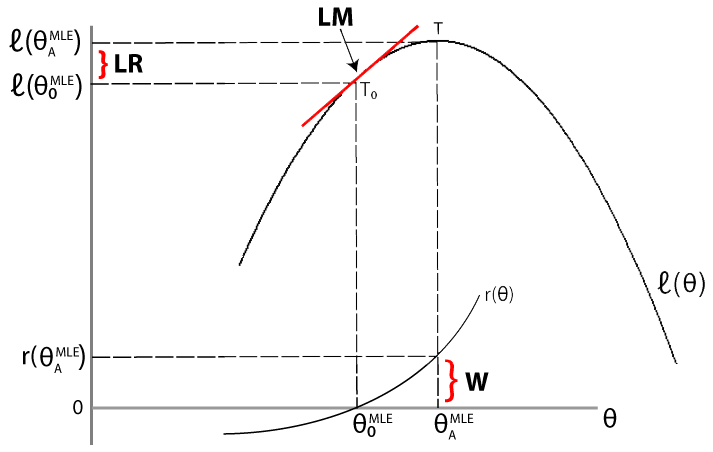
\includegraphics[width=0.8\textwidth]{fig/lr-Lm-w-test.png}
    \caption{LR/LM/W Test}
\end{figure}

\subsection{F检验}

可以使用F检验,检验\uline{线性约束条件}是否成立。假设约束模型$\theta_{k+1}=\theta_{k+2}=\dots=\theta_{k+m}=0$,即有$m$个约束条件,形式如下:
\begin{equation*}
    y_t = \theta_0 + \theta_1 x_{t,1} + \dots + \theta_{k} x_{t,k} + \varepsilon_t
\end{equation*}

无约束模型有如下形式:
\begin{equation*}
    y_t = \theta_0 + \theta_1 x_{t,1} + \dots + \theta_{k} x_{t,k} + \theta_{k+1} x_{t,k+1} + \dots + \theta_{k+m} x_{t,k+m} + \varepsilon_t
\end{equation*}

此时原假设$H_0: \theta_{k+1}=\theta_{k+2}=\dots=\theta_{k+m}=0$,其统计量为如下所示,此时$N$为样本容量,$m$为约束条件个数,其中$k+m+1$为无约束模型中回归参数的个数(包含常数$\theta_0$)
\begin{equation*}
    F = \frac{(SSE_{r} - SSE_{ur})/m}{SSE_{ur}/(N-(k+m+1))} \sim F(m,N-(k+m+1))
\end{equation*}

当$F > F_{\alpha}(m,N-(k+m+1))$时,拒绝原假设,即约束条件不成立。反之,当$F \leq F_{\alpha}(m,N-(k+m+1))$时,约束条件成立。

\begin{remark}
    在Python与Matlab中有如下模块:
    \begin{itemize}
        \item \href{https://www.statsmodels.org/stable/generated/statsmodels.regression.linear_model.RegressionResults.compare_f_test.html}{Python: compare\_f\_test}
    \end{itemize}
\end{remark}

\subsection{似然比检验(LR)}

似然比(Likelihood ratio)检验认为,如果约束条件成立,可理解为约束前后没有变化,那么两个模型估计出的似然函数值应该近似相等。若$\theta_{r}$为约束模型(Restricted)的系数,其中$\theta_{r} = (\theta_1,\dots,\theta_k,\theta_{k+1}=0,\dots,\theta_{k+m}=0)$,共有$m$个系数被为0,即有$m$个约束条件。而$\theta_{ur} = (\theta_1,\dots,\theta_{k+m})$为无约束模型(Un-restricted)系数,可计算似然比为:
\begin{equation*}
    LR = -2\ln \left[ \frac{L(\theta_{r})}{L(\theta_{ur})} \right]
    = 2\left[ \ln L(\theta_{ur}) - \ln L(\theta_{r}) \right]
    \sim \chi^2(m)
\end{equation*}

原假设($H_0$)为约束模型$\theta_r$(小模型)对于数据的拟合与非约束模型(大模型)没有差别,$\theta_{k+1}=\theta_{k+2}=\dots=\theta_{k+m}=0$,即约束条件成立。拒绝原假设,约束条件不成立,即非约束模型(大模型)优于约束模型(小模型)。具体而言,当$LR \geq \chi_{\alpha}^2(m)$时,拒接原假设,非约束模型$\theta_{ur}$优于约束模型$\theta_{r}$。

\begin{remark}
    在Python与Matlab中有如下模块:
    \begin{itemize}
        \item \href{https://www.statsmodels.org/dev/generated/statsmodels.regression.linear_model.OLSResults.compare_lr_test.html}{Python: compare\_lr\_test}
        \item \href{https://www.mathworks.com/help/econ/lratiotest.html}{Matlab: lratiotest}
    \end{itemize}
\end{remark}

\subsection{拉格朗日乘子检验(LM)}

拉格朗日乘子检验(Lagrange multiplier test)或称得分检验(Score test),其中ARCH检验中的LM检验,为特例。

\begin{remark}
    在Python与Matlab中有如下模块:
    \begin{itemize}
        \item \href{https://www.statsmodels.org/stable/generated/statsmodels.regression.linear_model.RegressionResults.compare_lm_test.html}{Python: compare\_lm\_test}
        \item \href{https://www.mathworks.com/help/econ/lmtest.html}{Matlab: lmtest}
    \end{itemize}
\end{remark}

\subsection{沃尔德检验(Wald)}

沃尔德检验的优点是只需要估计无约束模型,即当约束模型估计困难时,尤为适用。并且F检验和LR检验只适用于检验线性约束条件,而沃尔德检验\uline{适用于线性与非线性约束条件}的检验。其原理如上图所示,测量无约束估计量(参数)与约束估计量(参数)之间的距离。

原假设$H_0$同样为$\theta_{k+1}=\theta_{k+2}=\dots=\theta_{k+m}=0$,即约束条件成立,约束模型与无约束模型没有差别。

\begin{remark}
    在Python与Matlab中有如下模块:
    \begin{itemize}
        \item \href{https://www.statsmodels.org/stable/generated/statsmodels.regression.linear_model.RegressionResults.wald_test.html}{Python: wald\_test}
        \item \href{https://www.mathworks.com/help/econ/waldtest.html}{Matlab: waldtest}
    \end{itemize}
\end{remark}

\section{线性回归模型}

“回归”(Regression)一词来最早源于生物学,英国生物统计学家高尔顿(Galton),为达尔文的表兄。其根据1078对父辈与子辈的身高的研究发现,虽然身材高大的父辈比身材矮的父辈倾向于有高的孩子,但平均而言,身材高大的父辈的孩子要矮些,而身材矮小的父辈的孩子要高些。即无论高个子或矮个子的后代,都有向均值方向拉回的倾向。其认为认为自然界有一种约束力,使得身高的分布不会向高矮两个极端发展,而是趋于回到中心,所以称为向均值回归(regression to the mean)。而现在一般指一整套统计流程,其中包括研究因变量与自变量之间的关系的分析研究,建立回归模型,并寻找其中的最佳拟合关系。

\subsection{回归模型分类}

对于回归模型(Regression Model),可分文参数回归(Parametric regression)与半参或非参回归(Semi/Non-parametric regression)。对于参数回归模型,对样本的总体分布做假设,其回归函数形式为已知,参数待定,外延容易,但形式呆板。如:
\begin{itemize}
    \item 线性回归(Linear regression)
    \item 逻辑回归(Logistic regression)
    \item 岭回归(Ridge regression)
    \item LASSO回归(Lasso regression)
    \item 多项式回归(Polynomial regression)
\end{itemize}

顾名思义,线性回归模型就是采用线性的方法对自变量与因变量建模。当自变量的数目只有一个时,称为简单线性回归(Simple linear regression,SLR)或一元线性回归。对于多个自变量,单一因变量的线性回归模型称为多元回归模型(Multiple regression,MLR),并为了区分多个因变量的情形,将其称之为多变量回归(Multivariate regression)。

对于参数的估计方法,最为常见方法为最小二乘法(Least squares),即通过最小化残差平方和估计参数。可分为线性最小二乘法与非线性最小二乘法。对于线性最小二乘法,又可分为:
\begin{itemize}
    \item 普通最小二乘法(Ordinary least squares,OLS)
    \item 加权最小二乘法(Weighted least squares,WLS)
    \item 广义最小二乘法(Generalized least squares,GLS)
\end{itemize}

而对于半参或非参回归(Semi/Non-parametric regression),不对样本的总体分布做假设。对函数的数学形式并无特殊的假定,外延困难,但拟合效果却较好。其中非参数回归基本方法如:
\begin{itemize}
    \item 核函数回归(Kernel regression)
    \item 最近邻函数法(Nearest-neighbor或K-nearest neighbors)
    \item 神经网络(Neural networks)
    \item 支持向量机(Support vector regression)
\end{itemize}

\subsection{一元线性回归}

\subsubsection{模型定义}

一元线性回归只包含一个自变量与一个因变量为最简单的线性回归形式。关于总体(Population)与样本(Sample)之间的关系,总体是我们希望研究的,如全中国人均工资与其教育水平之间的关系,但出于种种原因,我们只能从样本中推测这样的关系。方程(Function)描述的为理论关系,而模型(Model)则代表了实证中拟合关系。
\begin{itemize}
    \item 总体回归方程(Population regression function,PRF):为理论基础,无法直接观测。方程代表了$Y$的均值如何随着$X$的变化而变化,为总体均值的关系(或可以理解为代表性的个体)。如给定大学学历的中国人口,他们的平均工资是什么水平。因此并不指总体中的所有个体,每个大学毕业生的工资都达到某水平,显然这是错误的。
    \begin{equation*}
        \E\left[ Y_i \given X_i \right] = \beta_0 + \beta_1 X_i
    \end{equation*}
    \item 总体回归模型(Population regression model,PRM):对于样本容量为$n$的随机样本$(X_i,Y_i)$,假设其服从总体回归方程,由于现实世界是复杂的,模型只是现实问题的简化。因此第$i$次观察中,除了$X_i$之外影响$Y_i$的因素$\varepsilon_i$被称为\uline{误差}项或干扰项(无法观察)。由于误差的存在,使得$Y_i$偏离了$\E\left[ Y_i \given X_i \right]$。
    \begin{equation*}
        Y_i = \beta_0 + \beta_1 X_i + \varepsilon_i
    \end{equation*}
    \item 样本回归方程(Sample regression function,SRF):也被称为OLS回归线(OLS regression line),假设使用$\hat{\beta}_0$与$\hat{\beta}_1$为$\beta_0$与$\beta_1$的估计值。我们可以使用样本数据进行拟合并建立样本回归方程,得到真实值$Y_i$的样本拟合值$\hat{Y}_i$。
    \begin{equation*}
        \hat{Y}_i = \hat{\beta}_0 + \hat{\beta}_1 X_i
    \end{equation*}
    \item 样本回归模型(Sample regression model,SRM):最后通过样本回归模型,解释总体回归模型中所描述的实际问题($Y_i$),其中$e$为\uline{残差},观测实际值与拟合值之差。
    \begin{equation*}
        Y_i = \hat{\beta}_0 + \hat{\beta}_1 X_i + e_i
    \end{equation*}
\end{itemize}

\subsubsection{基本假定}

回归分析的主要目的,就是通过对样本分析,建立样本回归模型,从而尽可能准确的估计总体回归模型。由于在观察度量的过程中引入误差项(随机扰动项),只有对误差的分布做出假定,才能正确的确定估计参数的分布性质,从而进一步进行假设检验和区间估计。

\begin{assumption}
    线性于参数(Linearity in Parameters)

    总体回归模型的参数和随机扰动项为线性的(解释变量可以是非线性的),且模型是正确设置的。
    \begin{equation*}
        Y_i = \beta_0 + \beta_1 X_i + \varepsilon_i
    \end{equation*}

    \label{ols-assumnption-1}
\end{assumption}

\begin{assumption}
    随机抽样(Random Sampling)

    $(X_i,Y_i) \ilsep i=1,\dots,n$,代表样本容量为n的服从总体回归模型的随机样本。

    \label{ols-assumnption-2}
\end{assumption}

\begin{assumption}
    解释变量的样本有波动(Variation in $X$)

    样本中$X_i \ilsep i=1,\dots,n$的数值不为完全相同。若完全相同,则为一条垂直与X轴的直线,此时$\sum_{i=1}^{n} (X_i - \bar{X})^2 =0$,无法得到估计量$\hat{\beta}_1$。

    \label{ols-assumnption-3}
\end{assumption}

\begin{assumption}
    零条件均值(Zero Conditional Mean)

    给定解释变量的任何值,误差的期望值都为0。
    \begin{equation*}
        \E\left[ \varepsilon \given X \right] = 0
    \end{equation*}

    利用全期望公式还可以推导出无条件零均值:
    \begin{equation*}
        \E(\varepsilon) = \E\left[ \E \left( \varepsilon \given X \right) \right] = 0
    \end{equation*}

    \label{ols-assumnption-4}
\end{assumption}

根据假设\ref{ols-assumnption-4},还能得到性质$\Cov(X,\varepsilon)=0$。
\begin{proof}
    \begin{align*}
        \Cov(X,\varepsilon) &= \E\left[ \left(X - \E[X]\right) \left(\varepsilon - \E[\varepsilon]\right)\right] \\
        &= \E[X\varepsilon]- \E[X] \cancel{\E[\varepsilon]} \\
        &= \E[X\varepsilon]
    \end{align*}

    利用全期望公式可知$\E[X\varepsilon] = \E\left[\E(X\varepsilon \given X)\right]$,因此:
    \begin{align*}
        \Cov(X,\varepsilon) &= \E\left[\E(X\varepsilon \given X)\right] \\
        &= \E\left[ X \cancel{\E(\varepsilon \given X)}\right] \\
        &= 0
    \end{align*}

\end{proof}

\begin{assumption}
    同方差性(Homoskedasticity)

    给定解释变量的任何值,误差都具有相同的方差,即:
    \begin{equation*}
        \Var\left(\varepsilon_i \given X \right) = \sigma^2
    \end{equation*}

    \label{ols-assumnption-5}
\end{assumption}

根据上述假设,还能推导出如下性质:
\begin{itemize}
    \item 根据总方差定律(\ref{law-total-variance}),应有$\Var(\varepsilon) = \E\left[ \Var(\varepsilon \given X) \right] + \Var\left[ \cancel{\E(\varepsilon \given X)} \right]$,同时可以得到无条件方差$\Var\left(\varepsilon_i \right) = \sigma^2$
    \item 由于$\Var(\varepsilon \given X) = \E(\varepsilon^2 \given X) - \left[ \cancel{\E(\varepsilon \given X)} \right]^2$,因此$\E(\varepsilon^2 \given X) = \sigma^2$
    \item 如果假定$X$与$\varepsilon$独立,可以得到$\E(\varepsilon \given X) = \E(\varepsilon) =0$且$\Var(\varepsilon \given X)$,但独立性有时是过强的假定。
\end{itemize}

当$\Var(\varepsilon \given X)$取决于$X$时,则称误差项表现出异方差性(Heteroskedasticity),并且由于$\Var(\varepsilon \given X) = \Var(Y \given X)$,只要$\Var(Y \given X)$为$X$的函数时,就出现了异方差性。

\begin{assumption}
    误差正态性(Normality)

    总体误差$\varepsilon$独立于解释变量$X$且服从均值为0、方差为$\sigma^2$的正态分布:
    \begin{equation*}
        \varepsilon \sim N(0,\sigma^2)
    \end{equation*}

    因此$Y \given X \sim N(\beta_0+\beta_1 X, \sigma^2)$
    \label{ols-assumnption-6}
\end{assumption}

正态性假设提出为了假设检验与区间估计,正态性的假定不影响对参数的点估计,只有在确定参数的统计分布时才需要。此时可以将如上假设条件进行总结,如下图所示,通过假设\ref{ols-assumnption-1}至假设\ref{ols-assumnption-4}可以确保OLS估计量为线性无偏估计量),即$\E\left[\hat{\beta}_0\right]=\beta_0$与$\E\left[\hat{\beta}_1\right]=\beta_1$,即得到了估计量的均值。

通过上述假设,加上同方差假设\ref{ols-assumnption-5},可以推导OLS估计量的方差$\Var\left[\hat{\beta}_0\right]$与$\Var\left[\hat{\beta}_1\right]$。并且可以通过高斯·马尔科夫定理(Gauss-Markove Theorm),得到估计量的BLUE性质,即除了无偏,还是最优。根据高斯·马尔科夫定理(Gauss-Markov Theorem),在线性回归模型中,如果线性模型满足高斯马尔可夫假定,则回归参数(回归系数)的“最优线性无偏估计”(Best Linear Unbiased Estimator,BLUE)就是普通最小二乘法估计给出的参数估计量。其中的“最优”指比较其他估计量,方差最小(离散程度最小),因此也可称为“最小方差线性无偏估计”。

最后加上正态性假设\ref{ols-assumnption-6},构成了经典线性模型假设(Classical linear model assumptions,CLM),如上已知了OLS估计量的均值与方差,但并未确保其分布。由于OLS估计量为随机变量$Y_i$(由于包含不可观测的误差$\varepsilon_i$)的线性组合(和)。因此根据中心极限定理 (Central limit theorem),在大样本下,估计量将服从正态分布。而在小样本的情况下,只有正态性的假设,可能保证OLS估计量服从正态分布。

\begin{figure}[H]
    \centering
    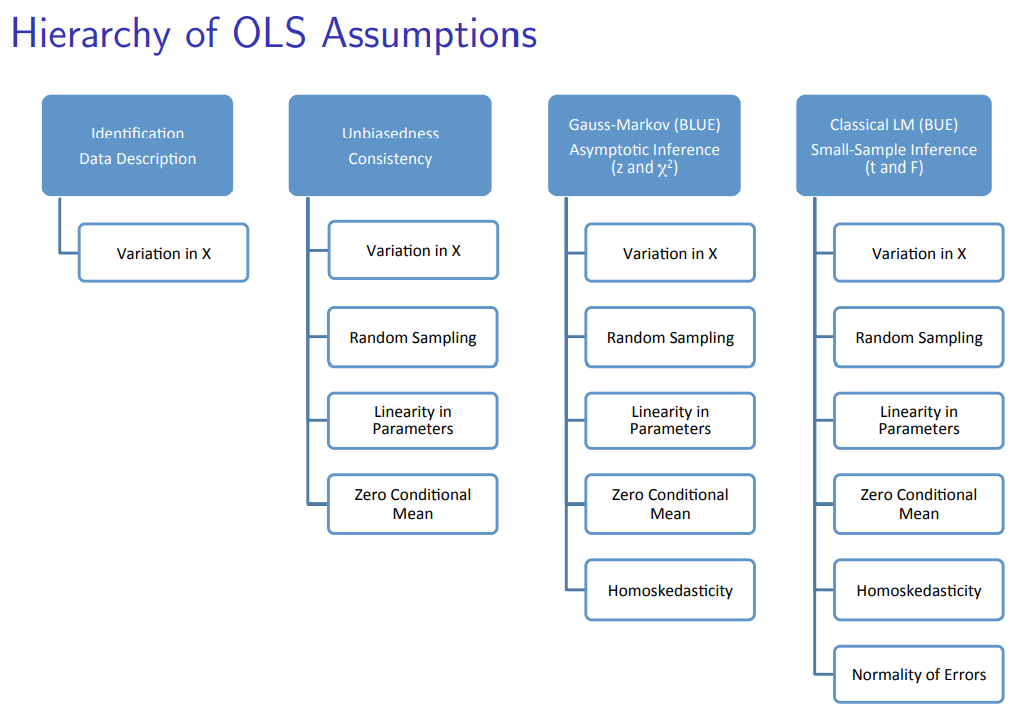
\includegraphics[width=0.8\textwidth]{fig/ols-assumptions.png}
    \caption{OLS基本假设}
    \label{fig:ols-assumptions}
\end{figure}

\subsubsection{普通最小二乘法(OLS)}

$\hat{Y}_i$为自变量或解释变量通过回归模型所得到的拟合值,在理想的估计方法下,应使得理论值$Y_i$和拟合值的$\hat{Y}_i$的差,即$e_i = Y_i - \hat{Y}_i$残差尽可能的小。由于得到的残差结果可能为正或为负,为了去除符号带来的影响,因此选择使用平方和作为衡量标准。定义如下函数$Q(\hat{\beta}_0, \hat{\beta}_1)$为残差的平方和函数,其中$\hat{\beta}_0$与$\hat{\beta}_1$为参数$\beta_0$与$\beta_1$(未知常数)的OLS估计值:
\begin{equation*}
    Q(\hat{\beta}_0, \hat{\beta}_1)
    = \sum_{i=1}^{n} e_i^2
    = \sum_{i=1}^{n} \left( Y_i - \hat{Y}_i \right)^2
    = \sum_{i=1}^{n} \left( Y_i - \hat{\beta}_0 - \hat{\beta}_1 X_i \right)^2
\end{equation*}

并希望其最小,则有:
\begin{equation*}
    \min Q(\hat{\beta}_0, \hat{\beta}_1) = \min \sum_{i=1}^{n} e_i^2
\end{equation*}

由$Q$对$\hat{\beta}_0$与$\hat{\beta}_1$求偏导可以得到OLS参数估计的两个一阶条件(First order conditions):
\begin{align*}
    \frac{\partial Q}{\partial \hat{\beta}_0} &= -2 \sum_{i=1}^{n} \left( Y_i - \hat{\beta}_0 - \hat{\beta}_1 X_i \right) = 0 \\
    \frac{\partial Q}{\partial \hat{\beta}_1} &= -2 \sum_{i=1}^{n} \left( Y_i - \hat{\beta}_0 - \hat{\beta}_1 X_i \right) X_i = 0
\end{align*}

求解一阶条件,即可得到回归系数的OLS估计$\hat{\beta}_0$与$\hat{\beta}_1$:
\begin{align*}
    \hat{\beta}_0 &= \bar{Y} - \hat{\beta}_1 \bar{X} \\
    \hat{\beta}_1 &= \frac{\sum_{i=1}^{n} \left(X_i - \bar{X}\right) \left(Y_i - \bar{Y}\right)}{\sum_{i=1}^{n} \left(X_i - \bar{X}\right)^2} \\
    &= \frac{\Cov(X,Y)}{\Var(X)} = \frac{\rho_{XY} \sigma_X \sigma_Y}{\Var(X)} = \rho_{XY} \frac{\sigma_Y}{\sigma_X}
\end{align*}

\begin{proof}
对于一式对$\hat{\beta}_0$求导,有:
\begin{gather*}
    \frac{\partial Q}{\partial \hat{\beta}_0} = -2 \sum_{i=1}^{n} \left( Y_i - \hat{\beta}_0 - \hat{\beta}_1 X_i \right) = 0 \\
    \sum_{i=1}^{n} Y_i - \sum_{i=1}^{n} \hat{\beta}_0 - \hat{\beta}_1 \sum_{i=1}^{n} X_i = 0 \\
    n \bar{Y} - n \hat{\beta}_0  - \hat{\beta}_1 n \bar{X} = 0 \\
    \hat{\beta}_0 = \bar{Y} - \hat{\beta}_1 \bar{X}
\end{gather*}

将$\hat{\beta}_0 = \bar{Y} - \hat{\beta}_1 \bar{X}$代入二式,推导可得:
\begin{gather*}
    \frac{\partial Q}{\partial \hat{\beta}_1} = -2 \sum_{i=1}^{n} \left( Y_i - \hat{\beta}_0 - \hat{\beta}_1 X_i \right) X_i = 0 \\
    \sum_{i=1}^{n} \left( Y_i X_i - \hat{\beta}_0 X_i - \hat{\beta}_1 X_i^2 \right) = 0 \\
    \sum_{i=1}^{n} \left( Y_i X_i - (\bar{Y} - \hat{\beta}_1 \bar{X}) X_i - \hat{\beta}_1 X_i^2 \right) = 0 \\
    \sum_{i=1}^{n} X_i Y_i - \bar{Y} \sum_{i=1}^{n} X_i + \hat{\beta}_1 \bar{X} \sum_{i=1}^{n} X_i - \hat{\beta}_1 \sum_{i=1}^{n} X_i^2 = 0 \\
    \sum_{i=1}^{n} X_i Y_i - \bar{Y} \sum_{i=1}^{n} X_i = \hat{\beta}_1 \left( \sum_{i=1}^{n} X_i^2 - \bar{X} \sum_{i=1}^{n} X_i \right) \\
    \hat{\beta}_1 = \frac{\sum_{i=1}^{n} X_i Y_i - n \bar{X} \bar{Y}}{\sum_{i=1}^{n} X_i^2 - n \bar{X}^2}
\end{gather*}

化简上述公式,对于分子有:
\begin{align*}
    \sum_{i=1}^{n} \left(X_i - \bar{X}\right) \left(Y_i - \bar{Y}\right)
    &= \sum_{i=1}^{n} \left( X_i Y_i - X_i\bar{Y} - \bar{X}Y_i + \bar{X}\bar{Y} \right) \\
    &=\sum_{i=1}^{n} X_i Y_i - \bar{Y} \sum_{i=1}^{n} X_i - \bar{X} \sum_{i=1}^{n} Y_i + n\bar{X}\bar{Y} \\
    &=\sum_{i=1}^{n} X_i Y_i - \bar{Y} n \bar{X} - \bar{X} n \bar{Y} + n\bar{X}\bar{Y} \\
    &=\sum_{i=1}^{n} X_i Y_i - n\bar{X}\bar{Y}
\end{align*}

对于分母有:
\begin{align*}
    \sum_{i=1}^{n} \left(X_i - \bar{X}\right)^2
    &= \sum_{i=1}^{n} \left( X_i^2 - 2 X_i\bar{X} + \bar{X}^2 \right) \\
    &= \sum_{i=1}^{n} X_i^2 - 2 \bar{X} \sum_{i=1}^{n} X_i + n\bar{X}^2 \\
    &= \sum_{i=1}^{n} X_i^2 - 2 n \bar{X}^2 + n\bar{X}^2 \\
    &= \sum_{i=1}^{n} X_i^2 - n \bar{X}^2 
\end{align*}

因此,将上述结果代入$\hat{\beta}_1$中,将使得$Q(\hat{\beta}_0,\hat{\beta}_1)$最小时的$\hat{\beta}_0$与$\hat{\beta}_1$应为:
\begin{align*}
    \hat{\beta}_0 &= \bar{Y} - \hat{\beta}_1 \bar{X} \\
    \hat{\beta}_1 &= \frac{\sum_{i=1}^{n} \left(X_i - \bar{X}\right) \left(Y_i - \bar{Y}\right)}{\sum_{i=1}^{n} \left(X_i - \bar{X}\right)^2} \\
    &= \frac{\Cov(X,Y)}{\Var(X)} = \frac{\rho_{XY} \sigma_X \sigma_Y}{\Var(X)} = \rho_{XY} \frac{\sigma_Y}{\sigma_X}
\end{align*}
\end{proof}

根据如上推导的OLS参数估计的一阶条件,还能得到下述三条代数性质。

\begin{property}
    点$\left(\bar{X},\bar{Y}\right)$总在OLS回归线上。

    \begin{equation*}
        \bar{Y} = \hat{\beta}_0 + \hat{\beta}_1 \bar{X}
    \end{equation*}

    \begin{proof}
        由一阶条件$\partial Q/\partial \hat{\beta}_0 = 0$可知$\hat{\beta}_0 = \bar{Y} - \hat{\beta}_1 \bar{X}$,显然有$\bar{Y} = \hat{\beta}_0 + \hat{\beta}_1 \bar{X}$。
    \end{proof}
    \label{ppt:ols-reg-line}
\end{property}

\begin{property}
    OLS残差的样本和、样本均值均为零。
    \begin{equation*}
        \sum_{i=1}^{n} e_i = 0
    \end{equation*}

    \begin{proof}
        已知$e_i = Y_i - \hat{Y}_i$,并根据上述性质\ref{ppt:ols-reg-line}与$\partial Q / \partial \hat{\beta}_0 = 0$的一阶条件可知:
        \begin{equation*}
            \sum_{i=1}^{n} e_i 
            = \sum_{i=1}^{n} \left(Y_i - \hat{Y}_i\right)
            = \sum_{i=1}^{n} \left(Y_i - \hat{\beta}_0 - \hat{\beta}_1 X_i \right) = 0
        \end{equation*}
    \end{proof}

    因此$\sum_{i=1}^{n} e_i=0$且$\E[e_i]=0$,并且等价的,拟合值$\hat{Y}_i$样本均值与${Y_i}$样本均值相等,即$\bar{\hat{Y}}=\bar{Y}$。
    \label{ppt:ols-error-mean}
\end{property}

\begin{property}
    解释变量与OLS残差的样本协方差为零。
    \begin{equation*}
        \sum_{i=1}^{n} X_i e_i = 0
    \end{equation*}

    \begin{proof}
        由上性质\ref{ppt:ols-error-mean}可知$\E[e_i]=0$,因此解释变量与残差的协方差应有:
        \begin{align*}
            \Cov(X_i,e_i) &= \E\left[\left(X_i - \E[X]\right)\left(e_i - \E[e]\right)\right] \\
            &= \E \left[e_i \left(X_i - \bar{X}\right) \right] \\
            &= \E[e_i X_i] - \bar{X}\E[e_i] \\
            &= \frac{1}{n} \sum_{i=1}^{n} e_i X_i
        \end{align*}
    
        根据一阶条件$\partial Q / \partial \hat{\beta}_1 = 0$可知:
        \begin{equation*}
            \sum_{i=1}^{n} X_i e_i = \sum_{i=1}^{n} X_i \left(Y_i - \hat{Y}_i\right) = \sum_{i=1}^{n} X_i \left(Y_i - \hat{\beta}_0 - \hat{\beta}_1 X_i\right) = 0
        \end{equation*}
    \end{proof}
\end{property}

\subsubsection{OLS估计量的期望与方差}

\begin{property}
    $\hat{\beta}_0$与$\hat{\beta}_1$为$Y_i$的线性组合

    如上文所证明$\hat{\beta}_1$为:
    \begin{equation*}
        \hat{\beta}_1 = \frac{\sum_{i=1}^{n} \left(X_i - \bar{X}\right) \left(Y_i - \bar{Y}\right)}{\sum_{i=1}^{n} \left(X_i - \bar{X}\right)^2}
    \end{equation*}

    利用性质:
    \begin{align*}
        \sum_{i=1}^{n} \left(X_i - \bar{X}\right) \left(Y_i - \bar{Y}\right)
        &= \sum_{i=1}^{n} \left( X_i - \bar{X} \right) Y_i - \bar{Y} \sum_{i=1}^{n} \left( X_i - \bar{X} \right) \\
        &= \sum_{i=1}^{n} \left( X_i - \bar{X} \right) Y_i - \bar{Y} \cancel{\left(\sum_{i=1}^{n} X_i - \sum_{i=1}^{n} \bar{X}\right)} \\
        &= \sum_{i=1}^{n} \left( X_i - \bar{X} \right) Y_i
    \end{align*}

    可得:
    \begin{equation*}
        \hat{\beta}_1 = \frac{\sum_{i=1}^{n} \left(X_i - \bar{X}\right) Y_i}{\sum_{i=1}^{n} \left(X_i - \bar{X}\right)^2}
    \end{equation*}

    令$b_i = \frac{\left(X_i - \bar{X}\right)}{\sum_{i=1}^{n} \left(X_i - \bar{X}\right)^2}$,那么可以将$\hat{\beta}_1$改写为:
    \begin{align*}
        \hat{\beta}_1 &= \frac{\sum_{i=1}^{n} \left(X_i - \bar{X}\right) Y_i}{\sum_{i=1}^{n} \left(X_i - \bar{X}\right)^2} \\
        &= \frac{(X_1 - \bar{X})Y_1}{\sum_{i=1}^{n} \left(X_i - \bar{X}\right)^2} Y_1 + \frac{(X_2 - \bar{X})}{\sum_{i=1}^{n} \left(X_i - \bar{X}\right)^2} Y_2 + \dots + \frac{(X_n - \bar{X})}{\sum_{i=1}^{n} \left(X_i - \bar{X}\right)^2} Y_n \\
        &= \sum_{i=1}^{n} b_i Y_i
    \end{align*}

    同时可以改写$\hat{\beta}_0$:
    \begin{equation*}
        \hat{\beta}_0 = \bar{Y} - \hat{\beta}_1 \bar{X}
        = \bar{Y} - \bar{X} \sum_{i=1}^{n} b_i Y_i
    \end{equation*}
    
    由上可见,显然$\hat{\beta}_0$与$\hat{\beta}_1$均为$Y_i$的线性组合。
\end{property}

\begin{property}
    $\hat{\beta}_0$和$\hat{\beta}_1$的期望与无偏性

    上文所定义的$b_i$,有如下性质:
    \begin{align*}
        \sum_{i=1}^{n} b_i
        &= \frac{\cancel{\sum_{i=1}^{n} \left(X_i - \bar{X}\right)}}{\sum_{i=1}^{n} \left(X_i - \bar{X}\right)^2} = 0 \\
        \sum_{i=1}^{n} b_i^2 
        &= \sum_{i=1}^{n} \left[ \frac{\left(X_i - \bar{X}\right)}{\sum_{i=1}^{n} \left(X_i - \bar{X}\right)^2} \right]^2
        = \sum_{i=1}^{n} \frac{\left(X_i - \bar{X}\right)^2}{ \left[ \sum_{i=1}^{n} \left(X_i - \bar{X}\right)^2 \right]^2} \\
        &= \frac{ \sum_{i=1}^{n} \left(X_i - \bar{X}\right)^2}{ \left[ \sum_{i=1}^{n} \left(X_i - \bar{X}\right)^2 \right]^2}
        = \frac{1}{\sum_{i=1}^{n} \left(X_i - \bar{X}\right)^2} \\
        \sum_{i=1}^{n} b_i X_i
        &= \frac{\sum_{i=1}^{n} \left(X_i - \bar{X}\right)X_i}{\sum_{i=1}^{n} \left(X_i - \bar{X}\right)^2}
        = \frac{\sum_{i=1}^{n} \left(X_i - \bar{X}\right) \left( X_i - \bar{X}\right)}{\sum_{i=1}^{n} \left(X_i - \bar{X}\right)^2} = 1
    \end{align*}

    此时,OLS估计量$\hat{\beta}_0$与$\hat{\beta}_1$为,$\beta_0$与$\beta_1$加上干扰项的线性组合:
    \begin{align*}
        \hat{\beta}_1
        &= \sum_{i=1}^{n} b_i Y_i 
        = \sum_{i=1}^{n} b_i \left( \beta_0 + \beta_1 X_i + \varepsilon_i \right) \\
        &=  \beta_0 \sum_{i=1}^{n} b_i + \beta_1 \sum_{i=1}^{n} b_i X_i + \sum_{i=1}^{n} b_i \varepsilon_i \\
        &= \beta_1 + \sum_{i=1}^{n} b_i \varepsilon_i
    \end{align*}

    可得$\hat{\beta}_0$与$\hat{\beta}_1$的期望为如下所示,当满足假设$\E(\varepsilon_i)=0$时,OLS估计量的无偏性得证:
    \begin{align*}
        \E\left( \hat{\beta}_1 \right)
        &= \beta_1 + \sum_{i=1}^{n} b_i \E(\varepsilon_i) = \beta_1 \\
        \E\left(\hat{\beta}_0 \right)
        &= \bar{Y} - \E\left( \hat{\beta}_1 \right) \bar{X}
        = \bar{Y} - \beta_1 \bar{X} = \beta_0
    \end{align*}
\end{property}

\begin{property}
    $\hat{\beta}_0$和$\hat{\beta}_1$的方差

    由于$X_i$为已知,可认为其为常数而非随机变量,其方差为零。根据总体回归模型$Y_i = \beta_0 + \beta_1 X_i + \varepsilon_i$,并且根据假设$\Var(\varepsilon_i \given X)$为同方差或常方差(方差为常数),即$\Var(Y_i) = \Var(Y_j) = \sigma^2 \ilsep \forall i,j$,可知:
    \begin{equation*}
        \Var(Y_i) = \cancel{\Var(\beta_0)} + \beta_1^2 \cancel{\Var(X_i)} + \Var(\varepsilon_i) = \sigma^2
    \end{equation*}

    由上文可知,令$b_i = \frac{\left(X_i - \bar{X}\right)}{\sum_{i=1}^{n} \left(X_i - \bar{X}\right)^2}$,可以将$\hat{\beta}_1$改写为$\hat{\beta}_1 = \sum_{i=1}^{n} b_i Y_i$,那么此时:
    \begin{align*}
        \Var\left(\hat{\beta}_1\right) &= \Var\left( \sum_{i=1}^{n} b_i Y_i \right) \\
        &= \sum_{i=1}^{n} b_i^2 \Var(Y_i) + 2b_i b_j \sum_{i\neq j} \Cov(Y_i,Y_j)
    \end{align*}

    由假设$Cov(\varepsilon_i,\varepsilon_j)=0$随机误差不相关,可得到$\Cov(Y_i,Y_j)=0$,最终结果如下所示。注意:当不满足随机误差不相关时,即$\Cov(Y_i,Y_j)$非零,其本应进入方差计算,但错误假设其为零,因此导致方差有偏且被低估,及检验假设时t值变大。
    \begin{align*}
        \Var\left(\hat{\beta}_1\right)
        &= \sum_{i=1}^{n} b_i^2 \Var(Y_i) \\
        &= \Var(Y_i) \sum_{i=1}^{n} b_i^2 \\
        &= \sigma^2 \sum_{i=1}^{n} b_i^2 \\
        &= \frac{\sigma^2}{\sum_{i=1}^{n} \left(X_i - \bar{X}\right)^2}
    \end{align*}

    注意:独立一定不相关,不相关不一定独立。此时相关指线性相关,即$\rho_{XY}=0$。例如在圆上的两点,显然不线性相关,但并非独立。并且有可以推导如下性质(在计算协方差时,只有$\Cov(Y_i,Y_i)=\Var(Y_i)=\sigma^2$项保留):
    \begin{align*}
        \Cov(\bar{Y},\hat{\beta}_1)
        &= \Cov \left( \frac{1}{n} \sum_{i=1}^{n} Y_i, \frac{\sum_{j=1}^{n} \left(X_j - \bar{X}\right) Y_j}{\sum_{i=1}^{n} \left(X_i - \bar{X}\right)^2} \right) \\
        &= \frac{1}{n} \frac{1}{\sum_{i=1}^{n} \left(X_j - \bar{X}\right)^2} \Cov \left( \sum_{i=1}^{n} Y_i, \sum_{j=1}^{n} \left(X_i - \bar{X}\right) Y_j \right) \\
        &= \frac{1}{n} \frac{1}{\sum_{i=1}^{n} \left(X_j - \bar{X}\right)^2} \sum_{i=1}^{n} \left(X_i - \bar{X}\right) \sigma^2 \\
        &= 0
    \end{align*}

    根据上述性质,$\hat{\beta}_0$方差有:
    \begin{align*}
        \Var(\hat{\beta}_0) 
        &= \Var\left( \bar{Y} - \hat{\beta}_1 \bar{X} \right) \\
        &= \Var \left(\bar{Y}\right) + \bar{X}^2 \Var\left( \hat{\beta}_1 \right) - 2\bar{X} \cancel{\Cov(\bar{Y},\hat{\beta}_1)} \\
        &= \Var\left( \frac{1}{n} \sum_{i=1}^{n} Y_i \right) + \bar{X}^2 \frac{\sigma^2}{\sum_{i=1}^{n} \left(X_i - \bar{X}\right)^2} \\
        &= \frac{1}{n^2} \left(\sum_{i=1}^{n} \Var(Y_i) + \cancel{\sum_{i \neq j} \Cov(Y_i,Y_j)}\right) + \bar{X}^2 \frac{\sigma^2}{\sum_{i=1}^{n} \left(X_i - \bar{X}\right)^2} \\
        &= \frac{\sigma^2}{n} + \frac{\sigma^2 \bar{X}^2}{\sum_{i=1}^{n} \left(X_i - \bar{X}\right)^2} \\
        &= \frac{\sigma^2 \sum_{i=1}^{n} \left(X_i - \bar{X}\right)^2}{n \sum_{i=1}^{n} \left(X_i - \bar{X}\right)^2}
        + \frac{n \sigma^2 \bar{X}^2}{n \sum_{i=1}^{n} \left(X_i - \bar{X}\right)^2} \\
        &= \frac{\sigma^2}{n \sum_{i=1}^{n} \left(X_i - \bar{X}\right)^2} \left[ \sum_{i=1}^{n} \left(X_i - \bar{X}\right)^2 + n\bar{X}^2 \right]
    \end{align*}

    由上已知:
    \begin{equation*}
        \sum_{i=1}^{n} \left(X_i - \bar{X}\right)^2
        = \sum_{i=1}^{n} X_i^2 - n \bar{X}^2 
    \end{equation*}

    代入上式,最终可得:
    \begin{equation*}
        \Var(\hat{\beta}_0)
        = \frac{\sigma^2 \sum_{i=1}^{n} X_i^2}{n \sum_{i=1}^{n} \left(X_i - \bar{X}\right)^2}
    \end{equation*}
\end{property}

\subsubsection{假设检验}

\subsubsection*{总体标准差已知}

在$\sigma$\uline{已知},并且满足假设的前提下,由上文推导可知$\hat{\beta}_1$服从如下分布:
\begin{equation*}
    \hat{\beta}_1 \sim N\left( \beta_1, \frac{\sigma^2}{\sum_{i=1}^{n} \left(X_i - \bar{X}\right)^2} \right)
\end{equation*}

那么即可构建检验统计量:
\begin{equation*}
    \frac{\hat{\beta}_1 - \beta_1}{s.e.(\hat{\beta}_1)} \sim N(0,1)
\end{equation*}

其中$\hat{\beta}_1$的标准误:
\begin{equation*}
    s.e.(\hat{\beta}_1) = \frac{\sigma}{\sqrt{\sum_{i=1}^{n} \left(X_i - \bar{X}\right)^2}}
\end{equation*}

\subsubsection*{总体标准差未知}

一般而言$\sigma$已知的情况较少,更多的情况$\sigma$\uline{未知},此时可以使用样本数据估计,得到$\sigma$的估计值$\hat{\sigma}$。具体而言,虽然$\sigma^2 = \Var(\varepsilon_i) = \E(\varepsilon_i^2) = \frac{1}{n} \sum_{i=1}^{n} \varepsilon_i$,但由于误差是无法观测的,因此无法使用。而残差可以从数据中计算出来,但若直接使用残差代替误差进行估计$\frac{1}{n} \sum_{i=1}^{n} e_i = \text{SSE}/n$,可以发现该估计量其实有偏的。由于在OLS中,需要满足两个约束,即如下两个一阶条件。
\begin{gather*}
    \sum_{i=1}^{n} \left( Y_i - \hat{Y}_i \right) = 0 \\
    \sum_{i=1}^{n} \left( Y_i - \hat{Y}_i \right) X_i = 0
\end{gather*}

因此OLS的残差只有$n-2$个自由度,即只需要知道残差中的$n-2$个,就可以通过两个一阶条件得到剩下的两个残差,因此若要得到$\sigma^2$的无偏估计量,就需要对自由度进行调整:
\begin{equation*}
    \hat{\sigma}^2 = \frac{\sum_{i=1}^{n} e_i^2}{n-2} = \frac{\text{SSE}}{n-2}
\end{equation*}

在假定满足的情况下,$\sigma^2$的的无偏估计有:
\begin{equation*}
    \E\left( \hat{\sigma}^2 \right) = \sigma^2
\end{equation*}

\begin{proof}
    首先需要注意区分误差$\varepsilon_i$与残差$e_i$,利用总体回归模型$Y_i = \beta_0 + \beta_1 X_i + \varepsilon_i$与样本回归模型$Y_i = \hat{\beta}_0 + \hat{\beta}_1 X_i + e_i$,将残差写为误差的函数。可以看到$e_i$不等于$\varepsilon_i$,但由于$\hat{\beta}_0$与$\hat{\beta}_1$的期望等于$\beta_0$与$\beta_1$,因此两者的期望值之差为零。
    \begin{align*}
        e_i &= Y_i - \hat{Y}_i \\
        &= Y_i - \hat{\beta}_0 + \hat{\beta}_1 X_i 
        = \left( \beta_0 + \beta_1 X_i + \varepsilon_i \right) - \hat{\beta}_0 + \hat{\beta}_1 X_i \\
        &= \varepsilon_i - \left( \hat{\beta}_0 - \beta_0 \right) - \left( \hat{\beta}_1 - \beta_1 \right) X_i
    \end{align*}
    
    对上式等式左右两侧取平均,并利用$\E\left(e_i\right)=0$,可知:
    \begin{equation*}
        0 = \bar{\varepsilon} - \left( \hat{\beta}_0 - \beta_0 \right) - \left( \hat{\beta}_1 - \beta_1 \right) \bar{X}
    \end{equation*}

    再与其相减,得到:
    \begin{align*}
        e_i &= \varepsilon_i - \left( \hat{\beta}_0 - \beta_0 \right) - \left( \hat{\beta}_1 - \beta_1 \right) X_i - \left[ \bar{\varepsilon} - \left( \hat{\beta}_0 - \beta_0 \right) - \left( \hat{\beta}_1 - \beta_1 \right) \bar{X} \right] \\
        &= \left( \varepsilon_i - \bar{\varepsilon} \right) - \left( \hat{\beta}_1 - \beta_1 \right) \left( X_i - \bar{X} \right)
    \end{align*}

    等式两侧平方:
    \begin{equation*}
        e_i^2 = 
        \left( \varepsilon_i - \bar{\varepsilon} \right)^2
        - 2\left( \varepsilon_i - \bar{\varepsilon} \right) \left( \hat{\beta}_1 - \beta_1 \right) \left( X_i - \bar{X} \right)
        + \left( \hat{\beta}_1 - \beta_1 \right)^2 \left(X_i - \bar{X}\right)^2
    \end{equation*}

    并对对等式两侧所有i求和,最终得到所需$\sum_{i=1}^{n} e_i^2$:
    \begin{equation*}
        \sum_{i=1}^{n} e_i^2 = 
        \sum_{i=1}^{n} \left( \varepsilon_i - \bar{\varepsilon} \right)^2 
        - 2 \left( \hat{\beta}_1 - \beta_1 \right) \sum_{i=1}^{n} \left( \varepsilon_i - \bar{\varepsilon} \right) \left( X_i - \bar{X} \right)
        + \left( \hat{\beta}_1 - \beta_1 \right)^2 \sum_{i=1}^{n} \left( X_i - \bar{X} \right)^2
    \end{equation*}

    对每一项求期望,第一项有:
    \begin{align*}
        \E \left[ \sum_{i=1}^{n} \left( \varepsilon_i - \bar{\varepsilon} \right)^2 \right]
        &= \E \left[ \sum_{i=1}^{n} \left( \varepsilon_i^2 - 2 \varepsilon_i \bar{\varepsilon} + \bar{\varepsilon}^2 \right) \right] \\
        &= \E \left( \sum_{i=1}^{n}  \varepsilon_i^2 \right) - 2 \E \left( \sum_{i=1}^{n}  \varepsilon_i \bar{\varepsilon} \right) + \E \left( \sum_{i=1}^{n} \bar{\varepsilon}^2 \right) \\
        &= \sum_{i=1}^{n} \E (\varepsilon_i)^2 - 2\E \left[ \sum_{i=1}^{n} \varepsilon_i \frac{\varepsilon_1 + \varepsilon_2 + \dots + \varepsilon_n}{n} \right] + n\E \left( \bar{\varepsilon}^2 \right) \\
        &= \sum_{i=1}^{n} \E (\varepsilon_i)^2 - \frac{2}{n} \E \left[ \left( \varepsilon_1 + \varepsilon_2 + \dots + \varepsilon_n \right) \sum_{i=1}^{n} \varepsilon_i \right] + n \E\left[ \left(\frac{\sum_{i=1}^{n} \varepsilon_i}{n} \right)^2 \right] \\
        &= \sum_{i=1}^{n} \Var(\varepsilon_i) - \frac{2}{n} \E \left( \sum_{i=1}^{n} \varepsilon_i \right)^2 + \frac{1}{n} \E \left( \sum_{i=1}^{n} \varepsilon_i \right)^2 \\
        &= \sum_{i=1}^{n} \Var(\varepsilon_i) - \frac{1}{n} \E \left( \sum_{i=1}^{n} \varepsilon_i \right)^2
    \end{align*}

    其中由于$\Cov(\varepsilon_i, \varepsilon_j)=0$,所有交乘项都为0,得到:
    \begin{equation*}
        \frac{1}{n} \E \left( \sum_{i=1}^{n} \varepsilon_i \right)^2
        = \frac{1}{n} \left[ \E(\varepsilon_1^2) + \E(\varepsilon_2^2) + \dots + \E(\varepsilon_n^2) \right]
        = \sigma^2
    \end{equation*}
    
    因此,对于第一项:
    \begin{equation*}
        \E \left[ \sum_{i=1}^{n} \left( \varepsilon_i - \bar{\varepsilon} \right)^2 \right] = n\Var(\varepsilon_i) - \sigma^2 = (n-1)\sigma^2
    \end{equation*}

    由于:
    \begin{equation*}
        \hat{\beta}_1 = \beta_1 + \frac{\sum_{i=1}^{n}\left(X_i - \bar{X}\right) \varepsilon_i}{\sum_{i=1}^{n} \left( X_i - \bar{X} \right)^2}
    \end{equation*}

    变换可得:
    \begin{equation*}
        \sum_{i=1}^{n}\left(X_i - \bar{X}\right) \varepsilon_i = \left( \hat{\beta}_1 - \beta_1 \right) \sum_{i=1}^{n} \left( X_i - \bar{X} \right)^2
    \end{equation*}

    将其代入第二项中:
    \begin{align*}
        - 2 \left( \hat{\beta}_1 - \beta_1 \right) \sum_{i=1}^{n} \varepsilon_i \left( X_i - \bar{X} \right)
        = -2 \left( \hat{\beta}_1 - \beta_1 \right)^2 \sum_{i=1}^{n} \left( X_i - \bar{X} \right)^2
    \end{align*}

    由于$\E\hat{\beta}_1\ = \beta_1$,因此$\Var\left( \hat{\beta}_1 \right) = \E \left[ \left( \hat{\beta}_i - \E\hat{\beta}_1 \right)^2 \right] = \E \left[ \left( \hat{\beta}_i - \beta_1 \right)^2 \right]$。并且由于$X_i$为已知,即求的实际为$\E(\cdot \given X)$条件期望,又因$\beta_1$为常数,因此对第二项取期望应有:
    \begin{align*}
        -2 \sum_{i=1}^{n} \left( X_i - \bar{X} \right)^2 \E \left[ \left( \hat{\beta}_1 - \beta_1 \right)^2 \right]
        &= -2 \sum_{i=1}^{n} \left( X_i - \bar{X} \right)^2 \Var\left(\hat{\beta}_1\right) \\
        &= -2 \sum_{i=1}^{n} \left( X_i - \bar{X} \right)^2 \frac{\sigma^2}{\sum_{i=1}^{n} \left(X_i - \bar{X}\right)^2} \\
        &= -2 \sigma^2
    \end{align*}

    对于第三项,同上可得:
    \begin{align*}
        \E \left[ \left( \hat{\beta}_1 - \beta_1 \right)^2 \sum_{i=1}^{n} \left( X_i - \bar{X} \right)^2 \right]
        &= \sum_{i=1}^{n} \left( X_i - \bar{X} \right)^2 \E \left[ \left( \hat{\beta}_1 - \beta_1 \right)^2 \right] \\
        &= \sum_{i=1}^{n} \left( X_i - \bar{X} \right)^2 \Var\left(\hat{\beta}_1\right) \\
        &= \sigma^2
    \end{align*}

    最终可得:
    \begin{equation*}
        \E\left( \sum_{i=1}^{n} e_i^2 \right) = (n-1)\sigma^2 - 2\sigma^2 + \sigma^2 = (n-2)\sigma^2
    \end{equation*}

    因此得到$\E\left(\hat{\sigma}^2\right)=\sigma^2$:
    \begin{equation*}
        \E\left( \hat{\sigma}^2 \right) 
        = \E \left( \frac{\sum_{i=1}^{n} e_i^2}{n-2} \right) 
        = \E \left( \frac{\text{SSE}}{n-2} \right) 
        = \sigma^2
    \end{equation*}
\end{proof}

使用$\hat{\beta}_1$的标准误去构建检验统计量,此时不再服从标准正态分布,而是t分布,如上文所述自由度为$n-2$:
\begin{equation*}
    \frac{\hat{\beta}_1 - \beta_1}{s.e.(\hat{\beta}_1)} \sim T_{n-2}
\end{equation*}

其中$\hat{\beta}_1$的标准误:
\begin{equation*}
    s.e.(\hat{\beta}_1) 
    = \frac{\hat{\sigma}}{\sqrt{\sum_{i=1}^{n} \left(X_i - \bar{X}\right)^2}}
    = \frac{\sqrt{\sum_{i=1}^{n} (Y_i - \hat{Y}_i)^2 / (n-2)}}{\sqrt{\sum_{i=1}^{n} (X_i - \bar{X})^2}}
\end{equation*}

构建检验统计量之后,就可以进行假设检验,提出假设:
\begin{align*}
    H_0&: \beta_1 = 0 \\
    H_1&: \beta_1 \neq 0
\end{align*}

给定显著性水平$\alpha$,当$\abs{T} > t_{\alpha/2}(n-2)$时,则说明检验统计量在$\alpha$显著性水平下显著,则拒绝原假设。

\subsubsection{总变差分解与拟合优度}

通过OLS估计得到了样本回归方程,此时我们希望衡量样本回归方程对数据拟合的好坏程度,这一指标通常被称为拟合优度(Goodness of fit)。回归分析之外,衡量给定分布对数据的的拟合优度有如下常见方法:
\begin{itemize}
    \item Bayesian information criterion(BIC)
    \item Akaike information criterion(AIC)
    \item Chi-square test
    \item Kolmogorov–Smirnov test
\end{itemize}

在回归分析中,常见的拟合优度指标为判定系数(Coefficient of determination)或称可决系数,使用$R^2$表示。可决系数衡量可解释的波动与总波动之比,即被解释变量$Y$中有多少样本波动,能被解释变量$X$的波动解释。并且由于SSR的大小与样本容量n的大小,以及变量的多少有关,因此不应仅采用SSR这一绝对量来衡量样本观测值与估计值偏离的大小,检验统计量应选择相对量。具体而言:
\begin{equation*}
    R^2 = \frac{\text{SSR}}{\text{SST}} = \frac{\text{SST}-\text{SSE}}{\text{SST}} = 1 - \frac{\text{SSE}}{\text{SST}}
\end{equation*}

另外,由于有:
\begin{equation*}
    \hat{Y}_i - \bar{Y} = \hat{\beta}_0 + \hat{\beta}_1 X_i - \left[ \hat{\beta_0} + \hat{\beta}_1 \bar{X} \right] = \hat{\beta}_1 \left( X_i - \bar{X} \right)
\end{equation*}

因此可将判定系数改写为:
\begin{equation*}
    R^2 = \frac{\text{SSR}}{\text{SST}}
    = \frac{\sum_{i=1}^{n} \left( \hat{Y}_i - \bar{Y}\right)^2}{\sum_{i=1}^{n} \left( Y_i - \bar{Y} \right)^2}
    = \hat{\beta}_1^2 \frac{\sum_{i=1}^{n} \left( X_i - \bar{X} \right)^2}{\sum_{i=1}^{n} \left( Y_i - \bar{Y} \right)^2}
    = \hat{\beta}_1^2 \frac{S_X^2}{S_Y^2}
\end{equation*}

其中定义\textbf{总平方和}(Sum of squares total,SST)或总离差平方和,SST衡量被解释变量观测值$Y_i$总变差的大小,即在样本中的离散程度,同时可以看到将SST除以自由度$n-1$就得到了$Y_i$的样本方差:
\begin{equation*}
    \text{SST} = \sum_{i=1}^{n} \left( Y_i - \bar{Y} \right)^2
\end{equation*}

\textbf{总残差平方和}(Error sum of squares,SSE),SSE衡量被解释变量观测值与估计值之间的总变差大小,其自由度为$n-k$
\begin{equation*}
    \text{SSE} = \sum_{i=1}^{n} \left( Y_i - \hat{Y}_i \right)^2
    = \sum_{i=1}^{n} e_i^2
\end{equation*}

\textbf{总回归平方和}(Regression sum of squares,SSR),SSR衡量被解释变量回归估计值的总变差大小,其自由度为$k-1$:
\begin{equation*}
    \text{SSR} = \sum_{i=1}^{n} \left( \hat{Y}_i - \bar{Y} \right)^2
\end{equation*}

\begin{property}
    SSR与$\Var(\hat{Y}_i)$

    对于$\hat{Y}_i$其方差应有:
    \begin{equation*}
        \Var(\hat{Y}_i) = \E \left[ \hat{Y}_i - \E(\hat{Y}_i) \right]^2
        = \frac{1}{n} \sum_{i=1}^{n} \left[ \hat{Y}_i - \E(\hat{Y}_i) \right]^2
    \end{equation*}

    由于$\bar{Y} = \hat{\beta}_0 + \hat{\beta}_1 \bar{X}$,可得:
    \begin{equation*}
        \E(\hat{Y}_i) = \frac{1}{n} \sum_{i=1}^{n} \hat{Y}_i
        = \frac{1}{n} \sum_{i=1}^{n} \left( \hat{\beta_0} + \hat{\beta}_1 X_i \right) = \hat{\beta}_0 + \hat{\beta}_1 \bar{X}
        = \bar{Y}
    \end{equation*}

    因此可以得到:
    \begin{equation*}
        \Var(\hat{Y}_i) = \frac{1}{n} \sum_{i=1}^{n} \left( \hat{Y}_i - \bar{Y} \right)^2 = \frac{\text{SSR}}{n}
    \end{equation*}
\end{property}

\begin{property}
    根据如上对SST、SSR与SSE的定义,那么总平方和满足如下分解,即总平方能分解为两部分,一部分为能被回归解释的变差,另一部为不能被回归解释的变差:
    \begin{equation*}
        \text{SST} = \text{SSR} + \text{SSE}
    \end{equation*}
\end{property}

\begin{proof}
    \begin{align*}
        \text{SST} &= \sum_{i=1}^{n} \left(Y_i - \bar{Y}\right)^2 \\
        &= \sum_{i=1}^{n} \left[(Y_i - \hat{Y}_i) + (\hat{Y}_i - \bar{Y})\right]^2 \\
        &= \sum_{i=1}^{n} \left(Y_i - \hat{Y}\right)^2
        + 2\sum_{i=1}^{n} \left(Y_i - \hat{Y}_i\right)\left(\hat{Y}_i - \bar{Y}\right)
        + \sum_{i=1}^{n} \left(\hat{Y}_i - \bar{Y}\right)^2 \\
        &= \text{SSR} + 2\sum_{i=1}^{n} \left(Y_i - \hat{Y}_i\right)\left(\hat{Y}_i - \bar{Y}\right) + \text{SSE} \\
        &= \text{SSR} + 2\sum_{i=1}^{n} e_i \left[(\hat{\beta}_0 + \hat{\beta}_1 \hat{X}) - (\hat{\beta}_0 + \hat{\beta}_1 X_i)\right] + \text{SSE} \\
        &= \text{SSR} + 2\hat{\beta}_1 \sum_{i=1}^{n} e_i \left(X_i-\bar{X}\right) + \text{SSE} \\
        &= \text{SSR} + 2\hat{\beta}_1 \left(\sum_{i=1}^{n} e_i X_i - \bar{X}\sum_{i=1}^{n}e_i\right) + \text{SSE} \\
        &= \text{SSR} + \text{SSE}
    \end{align*}
\end{proof}


\subsection{多元线性回归}

一般对于多个自变量,单一因变量的线性回归模型称为多变量回归模型(Multiple regression或Multivariable regerssion)。对于多个因变量的回归模型称为多元回归模型(Multivariate regression)。

https://brilliant.org/wiki/multivariate-regression/


对于多变量回归模型,即单一因变量,多个自变量的回归模型应有:
\begin{equation*}
    \bm{Y = X \beta + \epsilon}
\end{equation*}

其中:
\begin{equation*}
    \begin{bmatrix}
        y_1 \\
        y_2 \\
        \vdots \\
        y_N
    \end{bmatrix} =
    \begin{bmatrix}
        1 & x_{1,1} & x_{1,2} & \dots & x_{1,K} \\
        1 & x_{2,1} & x_{2,2} & \dots & x_{2,K} \\
        \vdots & \vdots & \vdots & \ddots & \vdots \\
        1 & x_{N,1} & x_{N,2} & \dots & x_{N,K} \\
    \end{bmatrix}
    \begin{bmatrix}
        \beta_0 \\
        \beta_1 \\
        \vdots \\
        \beta_K
    \end{bmatrix} + 
    \begin{bmatrix}
        \epsilon_1 \\
        \epsilon_2 \\
        \vdots \\
        \epsilon_N
    \end{bmatrix}
\end{equation*}

\subsection{普通最小二乘法}

有n个观察值$\{x_i,y_i\}_{i=1}^{n}$,其线性回归模型有如下形式:
\begin{equation*}
    y_i = \beta_0 + x_{i,0} + \beta_1 x_{i,1} + \beta_2 x_{i2} + \dots + \beta_{p-1} x_{i,p-1} + \varepsilon_{i}
\end{equation*}

或改写为向量形式为如下所示,其中$\bm{x}_i = [x_{i,0},x_{i,2},\dots,x_{i,p-1}]^{T}$为$p\times 1$的列向量,$\bm{\beta}$也是$p \times 1$的列向量:
\begin{equation*}
    y_i = \bm{x}_{i}^{'} \bm{\beta} + \varepsilon_i
\end{equation*}

若写成矩阵形式,则有$\bm{Y}=[y_1,\dots,y_n]^{T}$、$\bm{\beta}=[\beta_1,\dots,\beta_n]^{T}$与$\bm{\varepsilon}=[\varepsilon_1,\dots,\varepsilon_n]^{T}$都为$n\times 1$的列向量,$\bm{X}$为$n\times p$,即$n$行$p$列的矩阵($x_{\cdot,0}=1$):
\begin{equation*}
    \bm{X} =
    \begin{bmatrix}
        1 & x_{1,1} & x_{1,2} & \cdots & x_{1,p-1} \\
        1 & x_{2,1} & x_{2,2} & \cdots & x_{2,p-1} \\
        1 & \vdots  & \vdots  & \ddots & \vdots    \\
        1 & x_{n,1} & x_{n,2} & \cdots & x_{n,p-1} \\
    \end{bmatrix}
\end{equation*}

此时矩阵形式有:
\begin{equation*}
    \bm{Y} = \bm{X} \bm{\beta} + \bm{\varepsilon}
\end{equation*}

【待补充】时间序列的估计,使用OLS,也需要满足OLS的假设,否则估计有偏

\subsection{广义最小二乘法}

广义最小二乘法(GLS),在放弃了同方差和序列相关的假设之下(准确地说是对误差项的条件方差作了更一般的假定),我们看到的回归式叫generalized regression model。在这种model里,GLS估计量是BLUE的。如果误差项的条件方差、协方差矩阵是已知的,GLS就是可行的,我们皆大欢喜。【存在异方差和序列相关】


简单举个例子,具体就不用符号了,推来推去太复杂。假设你有一把尺子,去测量一个物体的长度。你用同一把尺子测量n次,每次的测量误差就是这个尺子的误差(忽略其他因素),这就是我们所说的最小二乘里的同方差假定。现在你换一种方法,还是测量n次,但是你每次测量用的尺子精度不一样,有点大,有的小。这就是说所谓的“异方差”,这个时候你用普通最小二乘,就会导致估计不一致,这个时候,你想到一个办法就是,对于估计量中的样本,除以相应样本的那把尺子的误差,这样处理之后,就又变成同方差了。

作者:gurudk
链接:https://www.zhihu.com/question/37930145/answer/140471525
来源:知乎
著作权归作者所有。商业转载请联系作者获得授权,非商业转载请注明出处。

\section{时间序列}

\subsection{平稳性}

对于时间序列$\{r_t\}$,\textbf{强平稳}(Strongly stationary)或严格平稳(Strictly stationary),是指对于任意$t$和任意正整数$k$,发生在时间$(t_1,\dots,t_k)$上的资产收益率时间序列$(r_{t_1},\dots,r_{t_k})$,在经过$(t_1+t,\dots,t_k+t)$时间后,$(r_{t_1+t},\dots,r_{t_k+t})$仍有\uline{相同的联合分布},即经过t时间后,收益率的分布保持不变。

\textbf{弱平稳}(Weakly stationary)指对于时间序列$\{r_t\}$,$r_t$的均值平稳(Stationary in mean)与自身与滞后$l$阶的协方差平稳(Second-order stationary),即:
\begin{gather*}
    \E [r_t] = \mu \\
    \Cov (r_t, r_{t-1}) = \gamma_l
\end{gather*}

当时间序列$\{r_t\}$满足弱平稳时有,其均值$\mu$为常数,不随时间改变,而$\gamma_l$指依赖时间间距$l$的大小。同时当$l=0$时有,其方差$\Cov(r_t,r_t) = \Var(r_t) = \gamma_0$为与时间无关的常数,称为方差平稳性(Stationary in variance)。平稳性的强弱区别,在于弱平稳只要求期望与方差不变,即\uline{前两阶矩不变},而强平稳要求各阶距都不变。由于正态分布只需要两阶矩确认,因此时间序列$\{r_t\}$若是正态分布的,那么此时弱平稳与强平稳等价。

对于未知的概率分布,只需要进行大量重复实验,就可以有足够多的观测值来进行统计推断,即可以计算均值和方差等。但对于类似收益率的时间序列而言,某一天的收益率仅发生一次,不会重复发生。因此假设收益率序列满足\uline{弱平稳},此时其均值为常数$\E[r_t] = \mu$与时间$t$无关,因此可以利用一段时间的历史数据计算日收益率的均值。但需要注意,许多时候金融数据并不满足若平稳的条件。

协方差$\gamma_l = \Cov(r_t,r_{t-l})$称为$r_t$与滞后$l$阶的\textbf{自协方差}(Autocovariance)。按照定义可以得到当$l=0$时,自协方差等于方差,并利用弱平稳条件可以得到对称性:
\begin{align*}
    \gamma_0 &= \Var(r_t) \\
    \gamma_{-l} &= \Cov(r_{t},r_{t-(-l)}) = \Cov(r_{t-(-l)},r_{t}) \\
    &= \Cov(r_{t+l},r_{t}) = \Cov(r_{t},r_{t-l}) \\
    &= \gamma_{l}
\end{align*}

\subsection{自相关函数}

\subsubsection{相关系数}

根据定义,两个随机变量$X$与$Y$的相关系数定义为:
\begin{equation*}
    \rho_{X,Y} = \frac{\Cov(X,Y)}{\sqrt{\Var(X)\Var(Y)}}
    = \frac{\E\left[(X-\mu_x)(Y-\mu_y)\right]}{\sqrt{\E(X-\mu_x)^2 \E(Y-\mu_y)^2}}
\end{equation*}

对于样本$\{(x_t,y_t)\}_{t=1}^{T}$,其中样本均值为$\bar{x}=\sum_{t=1}^{T}x_t/T$与$\bar{y}=\sum_{t=1}^{T}y_t/T$:
\begin{equation*}
    \hat{\rho}_{x_t,y_t} = \frac{\sum_{t=1}^{T}(x_t-\bar{x})(y_t-\bar{y})}{\sqrt{\sum_{t=1}^{T}(x_t-\bar{x})^2 \sum_{t=1}^{T}(y_t-\bar{y})^2}}
\end{equation*}

\subsubsection{自相关函数}

假设$\{r_t\}$为若平稳收益率时间序列,使用相关系数的概念推广至$r_t$与其过去值$r_{t-l}$,那么$r_t$与$r_{t-l}$的相关系数称为$r_{t}$间隔为$l$的总体\textbf{自相关系数}(Autoregressive coefficient),即一个时间序列中当前节点,与其自身在不同时间节点的相关关系(相关系数):
\begin{equation*}
    \rho_l = \frac{\Cov(r_t,r_{t-l})}{\sqrt{\Var(r_t)\Var(r_{t-l})}} 
    = \frac{\Cov(r_t,r_{t-l})}{\Var(r_t)}
    = \frac{\gamma_l}{\gamma_0}
\end{equation*}

由于$\{r_t\}$为弱平稳收益率时间序列,应有$\Var(r_t) = \Var(r_{t-l})$。根据定义,$\rho_0=1$,根据自协方差的对称性,同样可得$\rho_{-l}=\rho_l$,并且值域为$-1 \leq \rho_l \leq 1$。一个弱平稳序列,当且仅当对所有$l>0$都有$\rho_l=0$时,其为序列不相关。

对于$\{r_t\}$,其样本均值为$\bar{r}=\frac{1}{T} \sum_{t=1}^{T} r_t$,\textbf{样本自协方差}(Sample autocovariance)为:
\begin{equation*}
    c_l = \frac{1}{n} \sum_{t=l+1}^{n} (r_t-\bar{r})(r_{t-l}-\bar{r})
\end{equation*}

\textbf{样本自相关系数}(Sample autocorrelation)为:
\begin{equation*}
    \hat{\rho}_l = \frac{c_l}{c_0} = \frac{\sum_{t=l+1}^{T}(r_t-\bar{r})(r_{t-l}-\bar{r})}{\sum_{t=1}^{T}(r_t-\bar{r})^2} \qquad 0 \leq l < T-1
\end{equation*}

若将$\hat{\rho}_l$视为$l$的方程,则称为\textbf{样本自相关函数}(sample Auto-Correlation Function,ACF),$\rho_l$为总体自相关函数。如下为存在明显趋势的时间序列,与存在明显周期性的时间序列的时间序列相关图(Correlogram)。通过相关图,可以清晰的看到ACF是如何随着$l$变化的:

\begin{figure}[H]
    \centering
    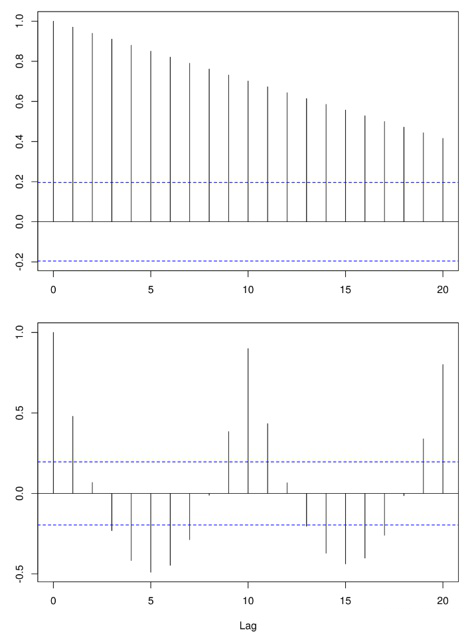
\includegraphics[width=0.5\textwidth]{fig/ts-trend.png}
    \caption{存在趋势的时间序列与存在周期的时间序列}
    \label{fig:ts-trend}
\end{figure}

\subsubsection{偏自相关系数(PACF)}

【待补充】

\subsubsection{如何对金融时间序列建模}

对于金融时间序列的建模,最重要的就是挖掘序列中不同间隔$l$的自相关性,透过相关图可以判断模型是否合适。\uline{由于金融时间序列中包含了相关性与随机噪声,因此如果模型很好的捕捉了相关性,那么原始时间序列与拟合之后的时间序列之间的残差应该等于随机噪声}。金融时间序列模型为解释时间序列相关性的数学模型,如上所述,其建模的核心为两点:
\begin{itemize}
    \item 一个优秀的模型应该能有效的刻画原始时间序列中不同间隔的相关性
    \item 衡量一个模型是否适合原始时间序列的标准为,考察原序列与拟合序列之间的残差序列是否可近似认为白噪声
\end{itemize}

对残差画出相关图,那么应该有其$\rho_0=1$,当$l\neq 0$时,$\rho_l=0$,随机噪声的自相关性均为0。

\begin{figure}[H]
    \centering
    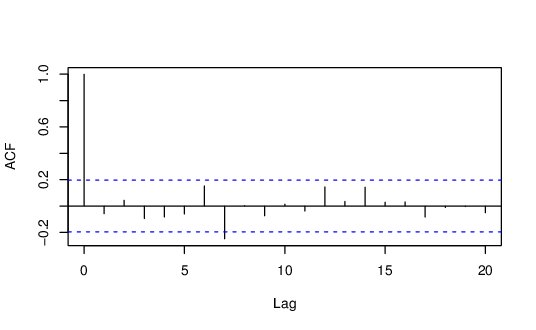
\includegraphics[width=0.6\textwidth]{fig/white-noise-acf.jpg}
    \caption{随机噪声的相关图}
    \label{fig:white-noise-acf}
\end{figure}

因此,在衡量对金融时间序列模型是否合适时,需先得到原时间序列与拟合序列之间的残差序列。然后依据残差序列的相关图,发现其是否含有未考虑的额外自相关性。若残差的相关图与上图类似,则可以认为该残差序列为一个随机噪声,即模型已经很好的捕捉了原时间序列中的自相关性。若残差的相关图体现了额外的自相关性,其将为改进已有的模型提供依据。

\subsection{自相关检验}

在线性模型中,需要满足一定的假设,如残差为独立。同样在时间序列当中,如果残差不独立,即自相关。如果时间序列变量之间独立,那么此时残差应该为白噪声,如果有特定的模式(如自相关),那么此时时间序列的独立性将不再满足。那么此时时间序列将如线性模型一样产生一定的问题,如参数估计量非有效(无偏,但不具备最小方差属性),变量的显著性检验失去意义,模型的预测失效。对于时间序列其他的自相关检验方法,一般有如下方法:
\begin{itemize}
    \item 观察ACF图
    \item Durbin-Watson test
    \item Ljung-Box Q test
    \item Lagrange Multiplier test
    \item Breusch-Godfrey Test (基于LM检验)
    \item Hildreth-Lu Procedure
\end{itemize}

\subsubsection{检验单个ACF}

若$\{r_t\}$为\textbf{独立同分布}(i.i.d.)序列,满足$\E(r_t^2)<\infty$,那么对于任意正整数$l$,有$\hat{p}_l$渐进的服从均值为$0$、方差为$1/T$的$N\sim(0,\frac{1}{T})$的正态分布。在更加一般的条件下,若$\{r_t\}$为\textbf{弱平稳}序列,满足$r_t = \mu + \sum_{i=0}^{q}\psi_i a_{t-i}$,其中$\phi_0=1$,$\{a_t\}$为均值为0的独立同分布变量序列,对于$l>q$,则有$\hat{p}_l$渐进的服从如下正态分布,称为Bartlett公式:
\begin{equation*}
    \hat{p}_l \sim N\left(0,\frac{\left( 1+2\sum_{i=1}^{q}\rho_i^2 \right)}{T} \right)    
\end{equation*}

对于正整数$l$,可以使用t检验(t-statistics)来检验$H_0: \rho_l =0$与$H_a: \rho_l \neq 0$检验统计量为:
\begin{equation*}
    t_{\hat{\rho}} = \frac{\hat{\rho}_l}{\sqrt{\left( 1+2\sum_{i=1}^{q}\hat{\rho}_i^2 \right)/T}}
\end{equation*}

如果$\{r_t\}$为平稳的高斯序列并满足当$j>l$时,$\rho_j=0$,则有他检验渐进的服从\uline{标准正态分布}。此时为双侧检验,假设显著性水平为$\alpha$,当$\abs{t_{\hat{\rho}}}>z_{\alpha/2}$时拒绝$H_0$,即在正态分布左右两端面积为$\alpha/2$的区域内拒绝$H_0$,而中间$1-\alpha$(置信水平)的区域不拒绝$H_0$,其中$Z_{\alpha/2}$为临界值(Critical value)。

临界值根据统计量的具体分布决定,由于统计量$t_{\hat{\rho}}$渐近服从标准正态分布。
对于双侧检验临界值$\pm Z_{\alpha/2}$为,使得标准正态分布PDF曲线下方阴影面积部分,左右两侧面积相加为$\alpha$的$Z$值。具体而言为标准正态分布CDF的$100(\alpha/2)$与$100(1-\alpha/2)$的两个分位点。例如当临界值为$\alpha=5\%$时,查表(Z-table)得知,为使得标准正态分布左右两侧阴影区域面积为$2.5\%$与$97.5\%$的两个临界值$Z$值,为$Z=\pm 1.96$。

\subsubsection{Durbin-Watson检验}

在检验残差中的自相关时,一般使用Ljung-Box检验,而非Durbin-Watson检验。这是由于DW检验只检验了滞后一阶的自回归,而很多时候自回归出现在更高阶的滞后项中,因此使用LB检验是更好的选择。对于Durbin-Watson检验而言,其原假设为残差中不存在自相关,而备择假设为残差中存在自相关,且为AR(1)过程:
\begin{align*}
    \text{H}_0: \ & \rho = 0 \\
    \text{H}_1: \ & \rho \neq 0
\end{align*}

若残差中存在自回归AR(1),即$\varepsilon_t = \rho \varepsilon_{t-1} + \mu_t$,则DW统计量有:
\begin{equation*}
    d = \frac{\sum_{t=2}^{T} (\varepsilon_t - \varepsilon_{t-1})^2}{\sum_{t=1}^{T} \varepsilon^2_t}
\end{equation*}

由于DW统计量近似于$d \approx 2(1-\hat{\rho})$,因此取值范围在$[0,4]$之间。当统计量:
\begin{itemize}
    \item 显著小于2时:有正的自相关
    \item 等于于2:无自相关
    \item 显著小于2:有负的自相关
\end{itemize}

\subsubsection{Ljung-Box Q检验}

在时间序列研究中,有两个著名的用于\uline{检测残差中自相关性}(残差的独立性)的\textbf{混成检验}(Portmanteau test),为Ljung-Box检验(或 Ljung-Box Q test)和Box-Pierce检验,其中Ljung-Box是Box-Pierce的扩展。目的在于\textbf{检验$r_t$的几阶自相关系数是否同时为零}。可以采用的方法还包括计算ACF和PCAF并观察其图像,但是无论是ACF还是PACF都只能考虑\uline{某一特定滞后阶数}的自相关,BP检验与LB检验则是基于\uline{一系列滞后阶数}。Box和Pierce(1970)检验统计量为:
\begin{equation*}
    Q^{*}(m) = T\sum_{i=1}^{m} \hat{\rho}_{l}^{2}
\end{equation*}

$Q^{*}(m)$渐进地服从自由度为$m$的$\chi^2$分布,\uline{检验原假设为无显著序列相关(自相关)}(即残差序列独立),而备择假设为有显著的序列相关性(残差序列非独立)。即当\textbf{接受原假设}$H_0$时,则代表该时间序列有没有显著的序列相关性:
\begin{align*}
    H_0&: \rho_1=\dots=\rho_{m}=0 \\
    H_1&: \text{对于某}\; i \in \{1,\dots,m\},\rho_i \neq 0
\end{align*}

Ljung和Box(1978)提高有限样本时的检验功效,修改后的统计量如下所示。临界值为$\alpha$,则有当$Q(m)>\chi_{\alpha}^{2}$时拒绝$H_0$,$\chi_{\alpha}^{2}$为自由度为$m$的$\chi^{2}$分布的$100-(1-\alpha)$的分位点,或当$p$值小于显著性水平$1-\alpha$时拒绝$H_0$。
\begin{equation*}
    Q(m) = T(T+2) \sum_{i=1}^{m} \frac{\hat{\rho}_{l}^{2}}{T-l}
\end{equation*}

\subsection{自相关处理}

当发现了残差中存在自相关,主要有如下三种转换
\begin{itemize}
    \item Cochrane-Orcutt Procedure
    \item Hildreth-Lu Procedure
    \item First Differences Procedure Section
\end{itemize}

https://online.stat.psu.edu/stat501/lesson/14/14.3

\subsection{白噪声与线性时间序列}

\subsubsection{白噪声与随机游走}

当$\{\omega_t\}$为一个有限均值和有限方差的\textbf{独立同分布}(Independent and identically distributed,iid)随机变量序列,则称其为\textbf{白噪声}(White noise)序列。独立同分布指一组随机变量$X_t$中,每个变量的概率分布都相同(均值方差等相同),显然满足平稳性要求。且白噪声满足序列不相关,相互独立,即$\omega_i$的取值不影响$\omega_j$的取值。对于白噪声序列,有其所有$l \neq 0 $的自相关函数(ACF)都为零$\rho_l = 0$。若$\omega_t$服从均值为$0$和方差为$\alpha^{2}$的正态分布,则称其为\textbf{高斯白噪声}(Gaussian white noise)。

若时间序列$\{x_t\}$满足$x_t = x_{t-1} + \omega_t$,其中$\omega_t$为均值为$0$,方差为$\sigma^2$的白噪声,则序列$\{x_t\}$为随机游走(Random walk)。由定义可知,在任意$t$时刻,$x_t$都为过去所有历史白噪声的综合,即:
\begin{equation*}
    x_t = \omega_{t} + \omega_{t-1} + \dots + \omega_0
\end{equation*}

因此随机游走的均值、方差和自协方差为为:
\begin{align*}
    \E(x_t) &= 0 \\
    \Var(x_t) &= \Var(\omega_{t}) + \Var(\omega_{t-1}) + \dots + \Var(\omega_{0}) \\
    &= t \times \Var(\omega_t) = t \sigma^2 \\
    \Cov(x_t,x_{t-l}) &= \Cov(\omega_{t}+ \omega_{t-1} + \dots + x_{t-l},x_{t-l}) \\
    &= \sum_{i=t-l+1}^{t} \Cov(w_i,x_{t-l}) + \Cov(x_{t-l},x_{t-l}) \\
    &= t\sigma^2
\end{align*}

由上可以看到,由于独立随机变量的房价可加性,方差为时间$t$的函数,因此随机游走并不满足平稳性。即随着时间增加,方差不断累积。自相关函数为如下所示,当一个时间序列足够长(t足够大),且间隔$l$足够小,则自相关系数近似为$1$。
\begin{align*}
    \rho_l(t) &= \frac{\Cov(x_{t},x_{t-l})}{\sqrt{\Var{x_{t}}}\sqrt{\Var{x_{t-l}}}} \\
    &= \frac{t\sigma^2}{\sqrt{t\sigma^2}\sqrt{(t-l)\sigma^2}} \\
    &= \frac{1}{\sqrt{1-l/t}}
\end{align*}

\subsubsection{线性时间序列}

如下时间序列称为线性时间序列(Linear time series),则有:
\begin{equation*}
    r_t = \mu + \sum_{i=0}^{\infty} \psi_i a_{t-i} = \mu + \psi_0 a_{t} + \psi_1 a_{t-1} + \psi_2 a_{t-2} + \dots
\end{equation*}

其中$\mu$为$r_t$的均值,$\pi_0=1$,并且$\{a_t\}$为均值为零的独立同分布随机变量序列,即$\{a_t\}$为白噪声序列。可以认为$a_t$表示该时间序列$t$时刻出现的新息(Innovation)或冲击(Shock)。其中$r_t$系数被称为$\psi$-权重,若$r_t$为弱平稳,则可以利用$\{a_t\}$的独立性得到:
\begin{equation*}
    \E(r_t) = \mu \qquad \Var(r_t) = \sigma_{a}^{2}\sum_{i=0}^{\infty} \psi_{i}^{2}
\end{equation*}

$\sigma_{a}^{2}$为$a_t$的方差,由于方差有限,应有$\Var(r_t)<+\infty$,所以$\{\psi_{i}^{2}\}$必须是收敛序列,当$i\rightarrow\infty$时,$\psi_{i}^{2}\rightarrow 0$,即随着$i$的增大,越早的历史扰动对当前时点的$r_t$影响越小,直至消失。$r_t$与间隔$l$的自协方差为:
\begin{align*}
    \gamma_l &= \Cov(r_t,r_{t-l})
    = \E\left[\left(r_t - \mu \right) \left(r_{t-l} - \mu \right) \right] \\
    &= \E\left[\left( \sum_{i=0}^{\infty} \psi_i a_{t-i} \right) \left( \sum_{j=0}^{\infty} \psi_j a_{t-l-j} \right) \right] \\
    &= \E \left[ \left( \psi_0 a_{t} + \psi_1 a_{t-1}  + \dots + \psi_l a_{t-l} + \psi_{l+1} a_{t-l-1}  + \dots \right) \left( \psi_0 a_{t-l} + \psi_1 a_{t-l-1} + \dots \right) \right] \\
    &= \E \left( \psi_l \phi_0 a_{t-l} a_{t-l} + \psi_{l+1} \phi_1 a_{t-l-1} a_{t-l-1}  + \dots \right)\\
    &= \sum_{i=0}^{\infty} \psi_{i+l} \psi_{i} \E(a_{t-l-i}^{2}) 
    = \sigma_{a}^{2} \sum_{i=0}^{\infty} \psi_i \psi_{i+l} 
\end{align*}

此时$\psi$-权重与$r_t$自相关系数有如下关系:
\begin{equation*}
    \rho_l = \frac{\Cov(r_t,r_{t-l})}{\Var(r_t)}
    = \frac{\gamma_l}{\gamma_0}
    = \frac{\sum_{i=0}^{\infty} \psi_i \psi_{i+l}}{1+ \sum_{i=0}^{\infty} \psi_i^2} \qquad l \geq 0
\end{equation*}

\subsection{自回归模型(AR)}

假设收益率$r_t$具有统计显著的,滞后一阶的自相关系数,说明在预测$r_t$时,$r_{t-1}$也发挥了较大的作用,因此可以建立简单的线性回归模型:
\begin{equation*}
    r_t = \phi_0 + \phi_1 r_{t-1} + a_t
\end{equation*}

其中$\{a_t\}$为均值为0,方差为$\sigma_{a}^2$的白噪音。此时由于$r_{t-1}$为自变量,$r_t$为因变量,与自身的滞后项进行回归,因此称为自回归模型(Autoregressive model,AR)。由于与自身滞后一阶自回归,因此称为一阶自回归模型或AR(1)模型。在过去收益率$r_{t-1}$已知条件下。有其均值与方差(波动来源于白噪声)有:
\begin{align*}
    \E(r_t \given r_{t-l}) &= \phi_0 + \phi_1 r_{t-1} \\
    \Var(r_t \given r_{t-l}) &= \E\left[\left(r_t - \E(r_t \given r_{t-1}) \right)^2 \given r_{t-l} \right] \\
    &= \E \left(a_t^2 \given r_{t-l} \right) = \E \left(a_t^2\right) \\
    &= \Var(a_t) = \sigma_{a}^{2}
\end{align*}

对AR(1)模型进行推广,因此p阶的AR模型表示在给定过去数据时,那么滞后1阶至p阶联合决定了$r_t$的条件期望:
\begin{equation*}
    r_t = \phi_0 + \phi_1 r_{t-1} +  \phi_2 r_{t-2} + \dots +  \phi_p r_{t-p}  + a_t
\end{equation*}

假设AR(1)是弱平稳的,则有$\E(r_t)=\mu$为常数,$\Var(r_t)=\gamma_0$为常数,$\Cov(r_t,r-l) = \gamma_l$是$l$的函数与$t$无关。对AR(1)模型两边取均值,得到:
\begin{equation*}
    \E(r_t) = \phi_0 + \phi_1 \E(r_t-1)
\end{equation*}

在平稳性的条件下$r_t$的期望为常数$\mu$,即$\E(r_t) = \E(r_{t-1}) = \mu$,因此有:
\begin{equation*}
    \E(r_t) = \mu = \frac{\phi_0}{1-\phi_1}
\end{equation*}

改写上式,利用$\phi_0 = \mu(1-\phi_1)$,代入AR(1)中有:
\begin{align*}
    r_t &= \mu(1-\phi_1) + \phi_1 r_{t-1} + a_t \\
    &= \mu + \phi_1 (r_{t-1}-\mu)+ a_t 
\end{align*}

将$r_{t-1} - \mu = \phi_1 (r_{t-2}-\mu)+ a_{t-1}$代入上式,得:
\begin{align*}
    r_t - \mu &= \phi_1 \left(\phi_1 (r_{t-2}-\mu)+ a_{t-1} \right) \\
    &= \phi_1^2 (r_{t-2}-\mu)+ \phi_1 a_{t-1} + a_t
\end{align*}

重复上述流程,重复代入,可以得到:
\begin{equation*}
    r_t - \mu = a_t + \phi_1 a_{t-1} + \phi_2 a_{t-2} + \dots = \sum_{i=0}^{\infty} \phi_{1}^{i} a_{t-i}
\end{equation*}

可以看到,AR(1)模型为一般线性时间序列$r_t = \mu + \sum_{i=0}^{\infty} \psi_i a_{t-i}$,当$\psi_i = \phi_{1}^{i}$时的特殊形式。由上式可知,$r_t-\mu$为$a_t$的线性组合,且$a_t$互相独立,那么应有$\E\left((r_{t}-\mu)a_{t+1}\right)=0$,因此有:
\begin{equation*}
    \Cov(r_{t-1},a_t) = \E\left[(r_{t-1} - \mu)(a_{t} - 0) \right] = 0
\end{equation*}

对AR(1)模型的两边取方差,常数的方差为零,注意包含协方差项,则有:
\begin{align*}
    \Var(r_t) &= \Var(\phi r_{t-1} + a_t) \\
    &= \phi_{1}^{2} \Var(r_{t-1}) + \sigma_{a}^{2} + \phi_1 \cancel{\Cov (r_{t-1},a_t)} \\
    &= \phi_{1}^{2} \Var(r_{t-1}) + \sigma_{a}^{2}
\end{align*}

此时由于平稳性,则有方差相等,即$\Var(r_{t}) = \Var(r_{t-1})$,因此:
\begin{equation*}
    \Var(r_{t}) = \frac{\sigma_{a}^{2}}{1-\phi_{1}^{2}}
\end{equation*}

此时由于方差是非负且有限的,那么则应有$\phi_{1}^{2}<1$。这样由AR(1)模型的弱平稳性可推得$-1<\phi_1<1$,为充分条件。反之,由$\phi_1<1$可推出AR(1)是弱平稳的,为必要条件。综上所述,AR(1)模型是弱平稳的\textbf{充分必要条件}是$\abs{\phi_1}<1$。

\subsubsection*{AR(1)的自相关系数}

已知当AR(1)时,有$\psi_i = \phi_1^i$,则$r_t$的方差应有:
\begin{equation*}
    \gamma_0 = \Var(r_t) = \sigma_{a}^{2}\sum_{i=0}^{\infty} \psi_{i}^{2}
    = \sigma_{a}^{2}\sum_{i=0}^{\infty} \left( \phi_1^{i}\right)^{2}
\end{equation*}

将$\phi_1^{i+l}$分解为$\phi_1^{i}\phi_1^{l}$,同时有自协方差$\gamma_l$:
\begin{equation*}
    \gamma_l = \sigma_{a}^{2} \sum_{i=0}^{\infty} \psi_i \psi_{i+l} 
    = \sigma_{a}^{2} \sum_{i=0}^{\infty} \phi_1^i \phi_1^{i+l} 
    = \sigma_{a}^{2} \phi_1^{l} \sum_{i=0}^{\infty} \phi_1^i \phi_1^{i} 
    = \sigma_{a}^{2} \phi_1^{l} \sum_{i=0}^{\infty} \left( \phi_1^i \right)^2
\end{equation*}

因此有当$l>0$时,有$\gamma_l=\phi_1 \gamma_{l-1}$或$\gamma_l=\phi_1^l \gamma_{0}$.同时AR(1)模型的自相关系数为($\rho_0=1$):
\begin{equation*}
    \rho_l = \frac{\Cov(r_t,r_{t-l})}{\Var(r_t)} = \phi_1^l
\end{equation*}

\subsubsection*{AR(2)模型}

AR(2)模型,如同AR(1)模型,为$r_t$自身与其滞后一阶与滞后两阶的函数:
\begin{equation*}
    r_t = \phi_0 + \phi_1 r_{t-1} + \phi_2 r_{t-2} + a_t
\end{equation*}

同理可以得到其期望:
\begin{equation*}
    \E(r_t) = \mu = \frac{\phi_0}{1-\phi_1-\phi_2}
\end{equation*}

将$\phi_0 = (1-\phi_1-\phi_2)\mu$代回AR(2)模型中,可得:
\begin{equation*}
    r_t - \mu = \phi_1(r_{t-1}-\mu) + \phi_2(r_{t-2}-\mu) + a_t
\end{equation*}

两边同乘以$(r_{t-l}-\mu)$,得到:
\begin{align*}
    (r_{t-l} - \mu)(r_t - \mu) = \phi_1 (r_{t-l}-\mu)(r_{t-1} - \mu)
    + \phi_2 (r_{t-l}-\mu)(r_{t-2} - \mu) + (r_{t-l}-\mu) a_t
\end{align*}

由于$\E\left[(r_{t-l} - \mu)a_t\right]$,对等式两边取期望则有:
\begin{equation*}
    \gamma_l = \phi_1 \gamma_{l-1} + \phi_2 \gamma_{l-2} \qquad l>0
\end{equation*}

对上式同除$\gamma_0$可得$r_t$的ACF性质有:
\begin{equation*}
    \rho_l = \phi_1 \rho_{l-1} + \phi_2 \rho_{l-2} \qquad l>0
\end{equation*}

并且有$\rho_1 = \phi_1 \rho_{0} + \phi_2 \rho_{-1} = \phi_1 \rho_{0} + \phi_2 \rho_{1} $,因此对于平稳的AR(2)序列$r_t$应有:
\begin{align*}
    \rho_0 &= 1 \\
    \rho_1 &= \frac{\rho_1}{1-\rho_2} \\
    \rho_l &= \phi_1 \rho_{l-1} + \phi_2 \rho_{l-2} \qquad l \geq 2
\end{align*}

令$B$为向后推移算子(back-shift operator),即有$B \times \rho_l = \rho_{l-1}$,有时也用$L$表示(Lag operator,滞后算子)。可以写成如下形式:
\begin{equation*}
    (1-\phi_1 B - \phi_2 B^2)\rho_l = 0
\end{equation*}

该方程对应二次多项式,或称为\uline{逆特征方程},并且方程的解,称为\uline{逆特征解}:
\begin{gather*}
    1 - \phi_1 x - \phi_2 x^2 = 0 \\
    x = \frac{\phi_1 \pm \sqrt{\phi_{1}^{2} + 4\phi_2}}{-2\phi_2}
\end{gather*}

假设方程的解(逆特征解)为$\omega_1$和$\omega_2$,在时间序列文献中,称这两个解的倒数即$1/\omega_1$与$1/\omega_2$为AR(2)模型的\textbf{特征根}(Characteristic roots),即逆特征解与特征解为互为倒数。AR(2)序列平稳的条件就是两个特征根的模都小于$1$,或逆特征根大于$1$,保证模型的自相关函数随着滞后$l$长度的增加,而趋向于$0$,即历史冲击的影响越来越小,为序列平稳的必要条件。

\subsubsection*{AR(p)模型}

同样将AR(1)与AR(2)的结果推广至AR(p)模型:
\begin{equation*}
    r_t = \phi_0 + \phi_1 r_{t-1} + \dots + \phi_p r_{t-p} + a_t
\end{equation*}

对于平稳的AR(p)序列,其均值为:
\begin{equation*}
    \E(r_t) = \mu = \frac{\phi_0}{1 - \phi_1 - \dots - \phi_p}
\end{equation*}

对应的逆特征方程有,为一个$p$次多项式,有$p$个解,其中可能既包含实数解也包含复数解,如上所述,这$p$个解的倒数称为该方程的特征根:
\begin{equation*}
    1 - \phi_1 x - \phi_2 x^2 - \dots - \phi_p x^p= 0
\end{equation*}

若方程的所有解得模都大于1,则有序列$\{r_t\}$是平稳的。或换言之,对于特征根,\uline{平稳性要求所有特征根的模都小于1}。对于AR(p)的平稳性有如下充分必要条件:
\begin{figure}[H]
\centering
    \begin{tikzpicture}
        \node (x) at (0,0) {AP(p)为弱平稳};
        \node (y) at (4,0) {所有特征根的模小于1};
        \path[->]
            (x) edge[bend left=30] node[pos=0.5,above] {充分条件} (y)
            (y) edge[bend left=30] node[pos=0.5,below] {必要条件} (x);
        \end{tikzpicture}
\caption{AR(p)为弱平稳的充分必要条件}
\end{figure}

\subsubsection*{特征方程与特征根}

\begin{example}
    斐波拉契(Fibonacci)数列

    斐波拉契数列满足$a_1=1$,$a_2=1$,且有$a_{n+2} = a_{n+1} + a_{n},\;,n=1,2,\dots$。试图将$a_n$改写为函数形式$f(n)$,则有$a_{n+2} = a_{n+1} + a_{n}$改写为$f(n+2) = f(n+1) + f(n)$。假设已求得该方程的两个特解$f_1$与$f_2$,对于任何实数$c_1$与$c_2$,$f= c_1 f_1 + c_2 f_2$也是方程的解:
    \begin{gather*}
        f_1(n+2) = f_1(n+1) + f_1(n) \\
        f_2(n+2) = f_2(n+1) + f_2(n)
    \end{gather*}

    两式相加,可以看到$f = c_1 f_1 + c_2 f_2$满足原式$f(n+2) = f(n+1) + f(n)$:
    \begin{equation*}
        c_1 f_1(n+2) + c_2 f_2(n+2) = \left( c_1 f_1(n+1) + c_2 f_2(n+1) \right) + \left( c_1 f_1(n)  + c_2 f_2(n) \right) \\
    \end{equation*}

    代入初始条件$a_1=a_2=1$,即$f(1)=f(2)=1$可以确定两个待定系数。将原式同除$f(n)$得到:
    \begin{equation*}
        \frac{f(n+2)}{f(n+1)} \cdot \frac{f(n+1)}{f(n)} - \frac{f(n+1)}{f(n)} - 1 = 0
    \end{equation*}

    若$\abs{f(n)}$为等比数列,则有上式变为$x^2-x-1=0$为特征方程,其解为$x_{1,2} = \frac{1\pm \sqrt{5}}{2}$,两个特征特解应为:
    \begin{equation*}
        f_1(n) = \left(\frac{1+\sqrt{5}}{2}\right)^{n-1} \quad
        f_2(n) = \left(\frac{1-\sqrt{5}}{2}\right)^{n-1}
    \end{equation*}
   
    该方程的通解应有:
    \begin{equation*}
        a_n = f(n) = c_1 f_1(n) + c_2 f_2(n) = 
        c_1 \left(\frac{1+\sqrt{5}}{2} \right)^{n-1} + c_2 \left( \frac{1-\sqrt{5}}{2} \right)^{n-1}
    \end{equation*}
    
    由初始条件$f(1)=f(2)=1$可得:
    \begin{gather*}
        c_1 + c_2 = 1 \\
        c_1 \left(\frac{1+\sqrt{5}}{2} \right) + c_2 \left( \frac{1-\sqrt{5}}{2} \right) = 1
    \end{gather*}
    
    联立求解可得:
    \begin{equation*}
        c_1 = \frac{1}{\sqrt{5}} \left(\frac{1+\sqrt{5}}{2} \right) \qquad
        c_2 = - \frac{1}{\sqrt{5}} \left(\frac{1-\sqrt{5}}{2} \right)
    \end{equation*}
    
    最终得证:
    \begin{equation*}
        a_n = \frac{1}{\sqrt{5}} \left[ \left(\frac{1+\sqrt{5}}{2} \right)^n - B\left( \frac{1-\sqrt{5}}{2} \right)^n \right]
    \end{equation*}
\end{example}

\subsection{移动平均模型(MA)}

移动平均(Moving average,MA)模型是另一个常见的线性时间序列模型。在自回归模型中,收益率$r_t$看作是给定阶数$p$下历史收益率序列的线性组合。而与自回归模型不同,移动平均模型将收益率$r_t$看作是历史白噪声的线性组合。可以认为移动平均模型是对漂移率之外的“随机噪声”建模,这些噪声可理解为不同时刻出现的影响收益率的新息或者冲击。通过对“噪声”建模来预测当前时刻$t$的“噪声”,再和漂移率结合,作为$t$时刻的收益率预测。

对于移动平均模型最简单的形式为1阶MA模型,简称MA(1)。其中$\{a_t\}$为白噪声序列,且$c_0$为常数:
\begin{equation*}
    r_t = c_0 + a_{t} - \theta_1 a_{t-1}
\end{equation*}

类似的有MA(2)为:
\begin{equation*}
    r_t = c_0 + a_{t} - \theta_1 a_{t-1} - \theta_2 a_{t-2}
\end{equation*}

MA(q)模型为:
\begin{equation*}
    r_t = c_0 + a_{t} - \theta_1 a_{t-1} - \dots - \theta_q a_{t-q}
\end{equation*}

\subsubsection*{平稳性}

\uline{MA模型总是弱平稳的},因为其为白噪声序列的有限线性组合,其前两阶矩是不随时间变化的。其中显然有$\E(r_t) = c_0$,对于MA(1)模型,其方差有:
\begin{align*}
    \Var(r_t) &= \Var(a_t) + \theta_1^2 \Var(a_{t-1}) - \theta_1 \Cov(a_t,a_{t-1}) \\
    & = \sigma_{a}^{2} + \theta_1^2 \sigma_{a}^{2} = (1 + \theta_1^2) \sigma_{a}^{2}
\end{align*}

即方差不随时间变化。同理,对于MA(q)模型也有:
\begin{equation*}
    \Var(r_t) = (1 + \theta_1^2 + \theta_2^2 + \dots ) \sigma_{a}^{2}
\end{equation*}

\subsubsection*{自相关系数}

对于MA(1)模型,其协方差有:
\begin{align*}
    \gamma_1 &= \E\left[(r_t - \mu)(r_{t-1} - \mu)\right] \\
    &= \E\left[(a_t - \theta_1 a_{t-1})(a_{t-1} - \theta_1 a_{t-2})\right] \\
    &= \E\left[ a_{t} a_{t-1} - \theta_1 a_{t} a_{t-2} - \theta_1 a_{t-1}^{2} + \theta_1^2 a_{t-1} a_{t-2} \right] \\
    &= -\theta_1 \E[a_{t-1}^2] = -\theta_1 \sigma_{a}^{2}
\end{align*}

且当$l>1$时,$\gamma_l=0$。因此其自相关系数有:
\begin{equation*}
    \rho_0 = 1 \qquad \rho_1=\frac{-\theta_1}{1 + \theta_1^2}
\end{equation*}

同样,当$l>1$时,$\rho_l=0$。因此,MA(1)模型的ACF在间隔为1以后是截尾的,同理MA(q)模型只与前$q$个滞后项线性相关,因此是一个有限记忆的模型。

【待验证】

\subsection{自回归移动平均模型(ARMA)}

自回归移动平均模型(Autoregressive moving average model,ARMA),将AR与MA模型的组合起来。ARMA(1,1)模型有($\phi_1 \neq \theta_1$):
\begin{equation*}
    r_t - \phi_1 r_{t-1} = \phi_0 + a_t - \phi_1 a_{t-1}
\end{equation*}

对于一般的ARMA(p,q)模型而言,即该模型有$p$阶滞后自回归项,与$q$阶滞后残差项:
\begin{equation*}
    r_t = \phi_0 + \sum_{i=1}^{p} \phi_i r_{t-i} + a_t - \sum_{i=1}^{q} \theta_i a_{t-i}
\end{equation*}

平稳时有均值为:
\begin{equation*}
    \E(r_t) = \frac{\phi_0}{1-\phi_1-\dots-\phi_p}
\end{equation*}

\subsection{自回归移动平均模型(ARIMA)}

将ARMA推广至允许其AR多项式以1作为它的特征根,则该模型变成了自回归求和移动平均模型(Autoregressive integrated moving average,ARIMA)。因为A多项式有单位根1,因此ARIMA模型称为是单位根非平稳的。

\subsection{确定模型的阶数}

在确定模型阶数时,常用的工具是使用信息量准则,包括赤池信息量准则(Akaike information criterion,简称 AIC,由日本统计学家赤池弘次创立)以及贝叶斯信息量准则(Bayesian information criterion,简称 BIC)。

其中$L$、$k$与$n$都为模型的似然函数,则有AIC与BIC定义为:
\begin{align*}
    AIC &= -2 \ln(L) + 2k \\
    BIC &= -2 \ln(L) + k\ln(n)
\end{align*}

从定义可知,AIC和BIC都由两部分组成,第一部分衡量模型的拟合度,第二部分为对参数个数的惩罚(防止过拟合)。当一个模型能够很好的解释(样本内)数据时,它的似然函数很大,因此第一项$-2\ln(L)$就会越小。且如果模型的参数越少,则第二项也越少,因此AIC和BIC总是越小越好。

【待添加】

\subsection{平稳性(单位根)检验}

对于时间序列的中的单位根检验,有大致一下三种检验方法:
\begin{itemize}
    \item DF检验:Dickey and Fuller(1979)
    \item ADF检验:Augmented Dickey-Fuller(1981)
    \item PP检验:Phillips and Perron(1988)
\end{itemize}

\subsubsection{DF检验}

假设模型有:
\begin{gather*}
    p_t = \phi_1 p_{t-1} + e_t \\
    p_t = \phi_0 + \phi_1 p_{t-1} + e_t
\end{gather*}

\begin{equation*}
    p_t = \phi_1 p_{t-1} + e_t
\end{equation*}

著名的单位单位根检验Dickey和Fuller(1979)的原假设为存在单位根,非平稳。而备择假设为该序列为平稳的,有:
\begin{gather*}
    H_0: \phi_1 = 1 \\
    H_a: \phi_1 < 1
\end{gather*}

使用最小二乘法估计T检验:
\begin{gather*}
    \hat{\phi}_1 = \frac{\sum_{t=1}^{T} p_{t-1}p_t}{\sum_{t=1}^{T} p_{t-1}^{2}} \\
    \hat{\sigma}_{e}^{2} = \frac{\sum_{t=1}^{T} \left(p_t - \hat{\phi}_1 p_{t-1} \right)^2}{T-1}
\end{gather*}

假设$p_0=0$,T为样本容量,此时\textbf{Dickey-Fuller检验}的统计量为:
\begin{equation*}
    DF = \frac{\hat{\phi}_1 - 1}{s.d.(\hat{\phi}_1)}
    = \frac{\sum_{t=1}^{T} p_{t-1} e_t}{\hat{\sigma}_{a} \sqrt{\sum_{t=1}^{T} p_{t-1}^{2}}} 
\end{equation*}

\subsubsection{ADF检验}

对于计量常用的AR(p)模型而言,为了检验AR(p)模型是否存在单位根,可以使用\textbf{扩展的Dickey-Fuller检验}(Augmented Dickey-Fuller)。其中原假设为$H_0: \beta=1$,而备择假设为$H_a: \beta<1$,模型有:
\begin{equation*}
    x_t = c_t + \beta x_{t-1} + \sum_{i=1}^{p-1}\phi_i \Delta x_{t-i} + e_t
\end{equation*}

$\Delta x_{i}= x_i -x_{i-1}$为$x_t$的差分数列,且$c_t$可以使零或者常数,或$c_t=\omega_0 + \omega_1 t$。ADF检验的统计量如下,其中$\hat{\beta}$为$\beta$的最小二乘估计:
\begin{equation*}
    ADF = \frac{\hat{\beta}-1}{s.e.(\hat{\beta})}
\end{equation*}

\subsection{一致的协方差矩阵估计(HC/HAC)}

对于同时同时研究两个时间序列$y_t$与$x_t$的关系,考虑如下线性回归:
\begin{equation*}
    y_t = \alpha + \beta x_t + e_t
\end{equation*}

误差项存在着序列相关或者条件异方差性,而分析的目标为回归系数$\alpha$与$\beta$做推断。在系数的最小二乘估计依然满足一致性的情况下,比较广泛的有两种方法能给出系数协方差的一致性估计(Consistent Covariance Matrix Estimation),有Eicker(1967)和White(1980)提出的异方差一致估计(HC),与\uline{Newey和West(1987)}提出的异方差及自相关一致估计(HAC),即对异方差与自相关都稳健的标准误。使用向量将回归模型改写:
\begin{equation*}
    y_t = \bm{x}_{t}^{'} \bm{\beta} + e_t \qquad t=1,2,\dots,T
\end{equation*}

其中$y_t$为因变量,$\bm{x}_{t} = (x_{1t},\dots,x_{kt})'$为包含常数项在内的$k$维向量,$\bm{\beta}_{t} = (\beta_{1t},\dots,\beta_{kt})'$为参数向量,$\bm{\beta}$那么最小二乘估计与协方差矩阵为:
\begin{equation*}
    \bm{\beta} = \left[ \sum_{t=1}^{T} \bm{x}_t \bm{x}_{t}^{'} \right]^{-1} \sum_{t=1}^{T} \bm{x}_t y_t \qquad 
    \Cov(\hat{\bm{\beta}}) = \sigma_{e}^{2} \left[ \sum_{t=1}^{T} \bm{x}_t \bm{x}_{t}^{'} \right]^{-1} 
\end{equation*}

当存在序列相关或条件异方差时,上述的协方差矩阵估计就不再是一致的,使得$\bm{\hat{\beta}}$的T统计量偏大。使用White(1980)的方法调整之后有,其中$\hat{e}_t = y_t - \bm{x}_{t}^{'} \bm{\hat{\beta}}$为$t$时刻的残差:
\begin{equation*}
    \Cov(\hat{\bm{\beta}})_{HC} = 
    \left[ \sum_{t=1}^{T} \bm{x}_t \bm{x}_{t}^{'} \right]^{-1} 
    \left[ \sum_{t=1}^{T} \hat{e}_{t}^{2} \bm{x}_t \bm{x}_{t}^{'} \right]
    \left[ \sum_{t=1}^{T} \bm{x}_t \bm{x}_{t}^{'} \right]^{-1} 
\end{equation*}

而Newey和West(1987)本质上是使用非参数的方法估计了$\left\{\sum_{t=1}^{T} \hat{e}_t \bm{x}_t \right\}$的协方差矩阵,有:
\begin{equation*}
    \Cov(\hat{\bm{\beta}})_{HAC} = 
    \left[ \sum_{t=1}^{T} \bm{x}_t \bm{x}_{t}^{'} \right]^{-1} 
    \hat{\mathbf{C}}_{HAC}
    \left[ \sum_{t=1}^{T} \bm{x}_t \bm{x}_{t}^{'} \right]^{-1} 
\end{equation*}

其中:
\begin{equation*}
    \hat{\mathbf{C}}_{HAC} = \sum_{t=1}^{T}\hat{e}_{t}^{2} \bm{x}_t \bm{x}_{t}^{'} + \sum_{j=1}^{l} \omega_j \sum_{t=j+1}^{T}\left( \bm{x}_t \hat{e}_t \hat{e}_{t-j} \bm{x}_{t-j}^{'} + \bm{x}_{t-j} \hat{e}_{t-j} \hat{e}_t \bm{x}_{t}^{'} \right)
\end{equation*}

$\omega_j$为权重函数,Newey和West建议$l$取$4(T/100)^{2/9}$的整部:
\begin{equation*}
    \omega_j = 1 - \frac{j}{l+1}
\end{equation*}

\begin{remark}
    在python中的\verb|statsmodels|进行回归时选择HAC选项即为Newey-West调整,即:
    \begin{verbatim}
        ols().fit(cov_type='HAC')
        some_reg_model.get_robustcov_results(cov_type='HAC')
    \end{verbatim}
\end{remark}

\section{条件异方差模型}

波动率有一个特性称之为波动率聚类(Volatility clustering),这意味着收益率的波动率是随时间变化的,不同阶段收益率的方差是不同的,这就是异方差性(heteroskedastic)。资产收益率表现出高波动伴随着高波动时期(大牛市或者股灾的时候),而低波动又往往伴随着低波动,因此\uline{波动率之间是存在序列相关性的},这就是“条件”一词的来源。将二者结合就有了条件异方差(Conditional heteroskedasticity)。

这样的特性对收益率序列的二阶平稳性假设提出了挑战,因此AR、MA与ARMA均不是不是条件异方差模型,也不考虑波动率聚类。针对这一特性,可对收益率的平方直接建模,即(G)ARCH模型。波动聚类仍然是一个必须要面对的问题,因此在实证中,使用滚动窗口,通过对在每个窗口中的一段收益率序列建模来规避掉波动聚类这个问题,即假设在每一小段窗口内的收益率序列是平稳的。

假设$r_t$服从平稳的ARMA(p,q)模型,即:
\begin{equation*}
    r_t = \phi_0 + \sum_{i=1}^{p} \phi_i r_{t-i} + a_t - \sum_{i=1}^{q} \theta_i a_{t-i}
\end{equation*}

对于增加了解释变量(外生变量)$x_{i,t}$的模型,其中$y_t$只是记号,表示去除解释变量影响后的调整收益率序列。
\begin{gather*}
    r_t=\mu_t + a_t \\
    \mu_t = \sum_{i=1}^{p} \phi_i y_{t-i} - \sum_{i=1}^{q} \theta_i a_{t-i} \\
    y_t = r_t - \phi_0 - \sum_{i=1}^{k} \beta_i x_{it}
\end{gather*}

对于给定$t-1$时刻,已知信息集合$F_{t-1}$时,$r_t$的条件均值与条件方差为如下所示。可以看到\uline{收益率的条件异方差即为新息的条件异方差},即考虑条件异方差需要对$a_t$新息进行建模:
\begin{align*}
    \mu_t &= \E(r_t \given F_{t-1}) \\
    \sigma_{t}^{2} &= \Var(r_t \given F_{t-1})
    = \E \left[ (r_t - \mu_t)^2 \given F_{t-1} \right] \\
    &= \E \left[ a_{t}^{2} \given F_{t-1} \right]
    = \Var(a_t \given F_{t-1})
\end{align*}

% 或写成通俗易懂的形式,如上所述$y_{t-j}$为提出解释变量影响后的$r_{t-j}$值:
% \begin{gather*}
%     r_t = \mu_t + a_t \\
%     \mu_t = \phi_0 + \sum_{i=1}^{k} \beta_i x_{it} + \sum_{i=1}^{p} \phi_i y_{t-i} - \sum_{i=1}^{q} \theta_i a_{t-i}
% \end{gather*}

\subsection{ARCH效应检验}

$a_t = r_t - \mu_t$为均值方程的残差,则可以用平方序列$a_t^2$来检验\textbf{条件异方差性},即所谓的\textbf{ARCH效应},即为残差平方$a_t^2$之间的序列相关性,或白噪声检测。第一种方式,可以使用\textbf{Ljung-Box}统计量$\{Q(m)\}$应用于序列$\{a_t^2\}$,参见Mcleod和Li(1983)。该检验的原假设是$\{a_t^2\}$序列的前$m$个间隔的ACF值都为零。

第二种方式,可以使用Engle(1982)中的拉格朗日乘子检验。对于\textbf{拉格朗日乘子检验}(Lagrange Multiplier Test,LM检验),等价于对如下线性回归中用F统计量检验$\alpha_i=0\;(i=1,\dots,m)$,即原假设有:
\begin{equation*}
    H_0: \alpha_1 = \dots = \alpha_m = 0
\end{equation*}

线性回归为:
\begin{equation*}
    a^2_t = \alpha_0 + \alpha_1 a^{2}_{t-1} + \dots + \alpha_m a^{2}_{t-m} + e_t \qquad t=m+1,\dots,T
\end{equation*}

$m$为正整数,$T$为样本容量,其中$e_t$为误差项,$\hat{e}_t$为上述线性回归最小二乘法估计的残差,$\bar{\omega}$为$a_t^2$的样本平均值。令:
\begin{gather*}
    SSR_0 = \sum_{t=m+1}^{T} (a_t^2 - \bar{\omega})^2 \qquad
    \bar{\omega} = \frac{1}{T} \sum_{t=1}^{T} a_t^2 \\
    SSR_1 = \sum_{t=m+1}^{T} \hat{e}_t^2
\end{gather*}

F统计量服从自由度为$m$的$\chi^2$分布,若$F>\chi_m^2(\alpha)$或F的p值小于$\alpha$则拒绝原假设,其中$\chi_m^2(\alpha)$为$\chi_m^2$上的$100(1-\alpha)$点:
\begin{equation*}
    F = \frac{(SSR_0-SSR_1)/m}{SSR_1/(T-2m-1)}
\end{equation*}

\begin{remark}
    ARCH效应检验或称为Engle's ARCH Test,如上所述应平方序列检验异方差性,详情见Engle(1982),与其他检验如Ljung-box Q-Test,拉格朗日乘数检验(Lagrange multiplier test或LM Test)也称为Score Test,在Python与Matlab中有如下模块可进行计算:
    \begin{itemize}
        \item \href{https://www.statsmodels.org/stable/generated/statsmodels.stats.diagnostic.acorr\_lm.html}{Python: acorr\_lm}(拉格朗日乘子序列相关检验)
        \item \href{https://www.statsmodels.org/stable/generated/statsmodels.tsa.stattools.q_stat.html#statsmodels.tsa.stattools.q_stat}{Python: q\_stat}
        \item \href{https://www.statsmodels.org/stable/generated/statsmodels.stats.diagnostic.acorr\_ljungbox.html}{Python: acorr\_ljungbox}(Ljung-Box序列相关检验)
        \item \href{https://www.statsmodels.org/stable/generated/statsmodels.stats.diagnostic.het\_arch.html}{Python: het\_arch}(Engle异方差检验)
        \item \href{https://www.statsmodels.org/stable/generated/statsmodels.stats.diagnostic.het\_breuschpagan.html}{Python: het\_breuschpagan}(Breusch-Pagan拉格朗日乘子异方差检验)
        \item \href{https://www.mathworks.com/help/econ/lbqtest.html}{Matlab: lbqtest}(Ljung-Box序列相关检验)
        \item \href{https://www.mathworks.com/help/econ/archtest.html}{Matlab: archtest}(Engle异方差检验)
    \end{itemize}
\end{remark}

\subsection{ARCH模型}

第一个尝试给波动率$\sigma_t$,即收益率的条件标准差,建模并提供系统框架的是由Engle(1982)提出的ARCH模型。基本思想为:
\begin{itemize}
    \item 资产收益率的扰动项$a_t = r_t - \E(r_t \given F_{t-1})$是序列不相关的,但不是独立的,若独立则不需要建模条件方差模型
    \item $a_t$的不独立性,描述为$\Var(r_t \given F_{t-1}) = \Var(a_t \given F_{t-1})$,即可以用$a_{t}^{2}$的滞后项的线性组合表示
\end{itemize}

具体而言,ARCH(m)模型如下所示。其中$\{\varepsilon_t\}$为均值为$0$方差为$1$的独立同分布白噪声序列:
\begin{gather*}
    a_t = \sigma_t \varepsilon_t \\
    \sigma_t^2 = \alpha_0 + \alpha_1 a_{t-1}^2 + \dots + \alpha_m a_{t-m}^2
\end{gather*}

\subsubsection{ARCH模型性质}

由于新息$a_t = r_t - \E(r_t \given F_{t-1})$,因此有其无条件均值与条件均值分别有:
\begin{align*}
    \E(a_t) &= \E(r_t) - \E[\E(r_t \given F_{t-1})] = \E(r_t) - \E(r_t) = 0 \\
    \E(a_t \given F_{t-1}) &= \E(\sigma_t \varepsilon_t \given F_{t-1}) = \varepsilon_t \E(\sigma_t \given F_{t-1}) = 0
\end{align*}

对于条件方差有性质\uline{提取已知量},即对于已知量,可以直接从条件期望中提出。具体而言,若$X$是$\mathcal{H}$可测的,应有:
\begin{equation*}
    \E[X Y\given \mathcal{H}] = X \E[Y \given \mathcal{H}] 
\end{equation*}

同时新息$a_t$的无条件方差,根据总期望定律与上述提取已知量($\sigma_{t}^{2}$为$F_{t-1}$可测)有:
\begin{align*}
    \Var(a_t) &= \E\left[\left(a_t - \E(a_t)\right)^2\right]
    = \E\left[ a_t^2 \right] \\
    &= \E\left[ \E(a_t^2 \given F_{t-1}) \right]
    = \E\left[ \E(\sigma_t^2 \varepsilon_t^2 \given F_{t-1}) \right] \\
    &= \E\left[ \sigma_t^2 \E( \varepsilon_t^2 \given F_{t-1}) \right] \\
    &= \E\left[ \sigma_t^2 \right] = \E \left[ \alpha_0 + \alpha_1 a_{t-1}^2 + \dots + \alpha_m a_{t-m}^{2} \right] \\
    &= \alpha_0 + \alpha_1 \E(a_{t-1}^{2}) + \dots + \alpha_m \E(a_{t-m}^{2}) \\
    &= \alpha_0 + \alpha_1 \Var(a_{t-1}) + \dots + \alpha_m \Var(a_{t-m})
\end{align*}

由于$a_t$是平稳过程,$\Var(a_{t}) = \Var(a_{t-1})$,且为正,因此系数有如下限制条件$\alpha_0 \geq 0$,$\alpha_1+\dots+\alpha_m<1$,在GARCH模型中即$\alpha$与$\beta$系数之和应小于$1$:
\begin{equation*}
    \Var(a_t) = \frac{\alpha_0}{1-\alpha_1 - \dots - \alpha_m}
\end{equation*}

由于$\varepsilon_t$独立,显然有:
\begin{equation*}
    \Var(\varepsilon_t) = \Var(\varepsilon_t \given F_{t-1}) = \E(\varepsilon_{t}^{2} | F_{t-1}) = 1
\end{equation*}

对于新息的方差有如下关系,可以证明$\sigma_{t}^{2}$即为\uline{新息的条件方差},可以看到其与滞后项有关,较大的历史冲击会导致较大的方差:
\begin{align*}
    \Var(a_t \given F_{t-1})
    &= \E(a_{t}^{2} \given F_{t-1})
    = \E(\sigma_{t}^{2} \varepsilon_{t}^{2} \given F_{t-1}) \\
    &= \sigma_{t}^{2} \E(\varepsilon_{t}^{2} \given F_{t-1}) \\
    &= \sigma_{t}^{2} = \alpha_0 + \alpha_1 a_{t-1}^2 + \dots + \alpha_m a_{t-m}^2
\end{align*}

同理可得收益率的条件方差也为$\sigma_{t}^{2}$:
\begin{align*}
    \Var(r_t \given F_{t-1}) &= \E\left[ \left( r_t - \E[r_t \given F_{t-1}] \right)^2 \given F_{t-1} \right] \\
    &= \E(a_{t}^{2} \given F_{t-1}) = \sigma_{t}^{2}
\end{align*}

同时有收益率的条件均值:
\begin{equation*}
    \E(r_t \given F_{t-1}) = \mu_t
\end{equation*}

\subsubsection{ARCH(1)模型}

对于ARCH(1)模型而言有,即只有一阶滞后项时,其中$\varepsilon_t$为均值为$0$方差为$1$的白噪声:
\begin{gather*}
    a_t = \sigma_t \varepsilon_t \\
    \sigma_{t}^{2} = \alpha_0 + \alpha_1 a_{t-1}^{2}
\end{gather*}

将$\sigma_t$带回$a_t$中可得:
\begin{equation*}
    a_t = \varepsilon_t \sqrt{\alpha_0 + \alpha_1 a_{t-1}^{2}}
\end{equation*}

由如上证明可知:
\begin{align*}
    \Var(a_t) &= \E\left[\sigma_{t}^{2}\right]
    = \E\left[ \alpha_0 + \alpha_1 a_{t-1}^{2} \right] \\
    &= \alpha_0 + \alpha_1 \E\left[a_{t-1}^{2}\right]
\end{align*}

由于$a_t$是平稳过程,并有$\E(a_t) = 0$,因此$\Var(a_t) = \Var(a_{t-1}) = \E(a_{t-1}^{2})$。因此有:
\begin{equation*}
    \Var(a_t) = \alpha_0 + \alpha_1 \Var\left(a_{t-1}\right)
\end{equation*}

可以看到ARCH(1)的方差$\Var(a_t)$,为一个AR(1)过程。由于方差为正,因此$0 \leq\alpha <1$:
\begin{equation*}
    \Var(a_t) = \frac{\alpha_0}{1-\alpha_1}
\end{equation*}

\subsubsection{建立ARCH模型}

【待添加】

\subsubsection{估计ARCH模型}

假设$\varepsilon_t$服从上述正态分布。对于条件概率分布$f(a_t \given F_{t-1})$,有:
\begin{gather*}
    \E(a_t \given F_{t-1}) = 0 \\
    \Var(a_t \given F_{t-1}) = \E(a_{t}^{2} \given F_{t-1}) = \sigma_{t}^{2} \E(\varepsilon_{t}^{2} \given F_{t-1}) = \sigma_{t}^{2}
\end{gather*}

因此条件概率分布函数有:
\begin{align*}
    f(a_t \given F_{t-1}) 
    &= \frac{1}{\sqrt{2\pi\sigma_{t}^{2}}} \exp\left[ - \frac{1}{2} \frac{(a_t - 0)^2}{\sigma_{t}^{2}} \right]\\
    &= \frac{1}{\sqrt{2\pi\sigma_{t}^{2}}} \exp \left[ -\frac{a_{t}^{2}}{2\sigma_{t}^{2}} \right]
\end{align*}

ARCH(m)的似然函数如下所示:
\begin{align*}
    f(a_1,\dots,a_T \given \bm{\alpha}) &= f(a_{T} \given F_{t-1}) f(a_{T-1} \given F_{t-2}) \dots f(a_{m+1} \given F_{m}) f(a_1,\dots,a_m \given \bm{\alpha}) \\
    &= \prod_{t=m+1}^{T} \frac{1}{\sqrt{2\pi\sigma_{t}^{2}}} \exp \left[ -\frac{a_{t}^{2}}{2\sigma_{t}^{2}} \right] \times f(a_1,\dots,a_m \given \bm{\alpha})
\end{align*}

其中$\bm{\alpha} = (\alpha_0,\alpha_1,\dots,\alpha_m)^{'}$。对于条件期望,应有如下性质:
\begin{equation*}
    \frac{f (a_1,\dots,a_m \cap a_{m+1},\dots,a_T \given \bm{\alpha})}{f(a_1,\dots,a_m \given \bm{\alpha})}
    = f(a_{m+1},\dots,a_T \given \bm{\alpha},a_1,\dots,a_m)
\end{equation*}

\begin{proof}
    令$a_1,\dots,a_m$为事件$X$,令$a_{m+1},\dots,a_T$为事件$Y$。因此原式为:
    \begin{align*}
        \frac{f( X \cap Y \given \bm{\alpha})}{f(X \given \bm{\alpha})} 
        &= \frac{f( X \cap Y \cap \bm{\alpha}) / f(\bm{\alpha}) }{f(X \cap \bm{\alpha}) / f(\bm{\alpha})} \\
        &= \frac{f( Y \cap X \cap \bm{\alpha})}{f(X \cap \bm{\alpha})} \\
        &= f(Y \given X \cap \bm{\alpha})
    \end{align*}
\end{proof}

因此得到条件似然函数:
\begin{equation*}
    f(a_{m+1},\dots,a_T \given \bm{\alpha},a_1,\dots,a_m) =
    \prod_{t=m+1}^{T} \frac{1}{\sqrt{2\pi\sigma_{t}^{2}}} \exp \left[ -\frac{a_{t}^{2}}{2\sigma_{t}^{2}} \right]
\end{equation*}

最大化如上联合分布,得到的估计称之为\uline{条件最大似然估计(MLE)},同时最大化条件似然函数\uline{等价于}最大化其对数,将条件似然函数(相乘),改写为对数似然函数(相加):
\begin{equation*}
    \mcl(a_{m+1},\dots,a_T \given \bm{\alpha},a_1,\dots,a_m)
    = \sum_{i=m+1}^{T} \left[ -\frac{1}{2}\ln(2\pi) - \frac{1}{2} \ln(\sigma_{t}^{2}) - \frac{1}{2} \frac{a_{t}^{2}}{\sigma_{t}^{2}} \right]
\end{equation*}

由于第一项为常数,因此对数似然函数可写为:
\begin{equation*}
    \mcl(a_{m+1},\dots,a_T \given \bm{\alpha},a_1,\dots,a_m) =
    \sum_{i=m+1}^{T} \left[ - \frac{1}{2} \ln(\sigma_{t}^{2}) - \frac{1}{2} \frac{a_{t}^{2}}{\sigma_{t}^{2}} \right]
\end{equation*}

或简单写成:
\begin{equation*}
    \mcl(\theta \given F_{t-1})
    = -\frac{T}{2}\ln(2\pi) - \frac{1}{2} \sum_{t=1}^{T} \ln(\sigma_{t}^{2}) - \frac{1}{2} \sum_{t=1}^{T} \frac{a_{t}^{2}}{\sigma_{t}^{2}}
\end{equation*}

在Python中可使用\verb|scipy.optimize.minimize|进行求解,最大化似然函数,即最小化负的对数似然函数(Neg Log-Likelihood)。

\subsection{GARCH模型}

Bollerslev(1986)年提出了对于ARCH模型的推广形式,称之为\textbf{广义ARCH模型}(Generalized Autoregressive Conditional Heteroskedasticity,GARCH)。对于对数收益率序列$r_t$,令$a_t = r_t - \mu_t$为$t$时刻的新息或冲击,则称$a_t$服从GARCH(m,s)模型,若$a_t$满足下式:
\begin{gather*}
    a_t = \sigma_t \varepsilon_t \\
    \sigma_{t}^{2} = \alpha_0 + \sum_{i=1}^{m} \alpha_i a_{t-i}^2 + \sum_{i=1}^{s} \beta_j \sigma_{t-j}^{2}
\end{gather*}

当$s=0$时,该模型就简化为ARCH(m)模型,同时将$\alpha_i$与$\beta_j$称为ARCH参数与GARCH参数。对于GARCH(1,1)模型有:
\begin{gather*}
    a_t = \sigma_t \varepsilon_t \\
    \sigma_{t}^{2} = \alpha_0 + \alpha_1 a_{t-1}^2 + \beta_1 \sigma_{t-1}^{2}
\end{gather*}

\subsubsection{建立GARCH模型}

在具体使用GARCH建模时,可以遵循如下步骤:
\begin{itemize}
    \item 使用ARMA对$\{r_t\}$建模以消除任何线性依赖,确定最优参数p和q(可以利用AIC/BIC来确定)
    \item 对上述模型的残差进行GARCH分析
    \item 如果残差中表现出显著的条件异方差,则给定一个波动模型GARCH(m,s)
    \item 使用历史数据对第一步中的ARMA(p,q) 和第三步中的GARCH(m,s) 进行联合参数估计
    \item 仔细检验第四步中拟合出的模型,如有必要则对其进行修改
\end{itemize}

\subsubsection*{注意}

由上述分析可知ARMA(p,q)的阶数,与GARCH(m,s)的阶数含义完全不同。ARMA是对于均值建模,而GARCH模型为$r_t$额波动率建模。

将均值模型与波动率模型拆开估计,与两者联合估计并不相同。若将其拆开估计,即先使用ARMA(p,q)对$r_t$建模,确定最优参数p和q,得到残差序列。而后使用GARCH模型对残差进行建模。由于此时因变量或被解释变量为残差,因此相当于使用均值为0的均值模型,与GARCH模型进行联合估计。即抛弃了联合估计中异方差对收益率序列的影响。在Tuey的3.5.4章节中也提到了两步估计的方法,认为是真是参数的一种近似,统计性质并没有得到很好的研究。

\subsubsection{(G)ARCH估计}

假设ARCH(1)模型:
\begin{align*}
    r_t &= \mu + a_t \\
    a_t &= \sigma_t \varepsilon_t \\
    \sigma^2 &= \alpha_0 + \alpha_1 a_{t-1}^{2}
\end{align*}

均值$\mu$为常数,且有$\varepsilon_t$服从均值为$0$方差为$1$的高斯分布,即高斯白噪声。此时待估参数为$\theta = (\mu,\alpha_0,\alpha_1)^{'}$,此时高斯似然函数有:
\begin{align*}
    \mcl( \theta \given r_t,F_{t-1})
    &= \frac{1}{\sqrt{2\pi\sigma_{t}^{2}(\theta)}} \exp \left[ -\frac{1}{2} \frac{a_{t}^{2}(\theta)}{\sigma_{t}^{2}(\theta)} \right] \\
    &= \frac{1}{\sqrt{2\pi\left(\alpha_0 + \alpha_1(r_{t-1}-\mu)^2\right)}} \exp \left[ -\frac{1}{2} \frac{(r_t - \mu)^2}{\alpha_0 + \alpha_1(r_{t-1}-\mu)^2} \right]
\end{align*}

对于更一般的情形,即$\mu$不再为常数,此时有:
\begin{align*}
    r_t &= \mu_t + a_t \\
    a_t &= \sigma_t \varepsilon_t
\end{align*}

假设$\varepsilon_t$为独立同分布,且满足$\E(\varepsilon_t)=0$和$\Var(\varepsilon_t)=1$,那么此时的高斯对数似然函数为如下所示。当$\varepsilon_t$不是高斯分布,那么此时称为\uline{准对数似然函数}(Quasi-log-likelihood)。
\begin{align*}
    \sum_{t=1}^{T} \ln \mcl_t(\theta)
    &= \sum_{t=1}^{T} \ln \left[ \frac{1}{\sqrt{2\pi\sigma_{t}^{2}(\theta)}} \exp \left( -\frac{1}{2} \frac{(r_t - \mu_t(\theta))^2}{\sigma_{t}^{2}(\theta)} \right) \right]
\end{align*}

在特定条件下,$\hat{\theta}_{\text{GQML}} = \arg \max \sum_{t=1}^{T} \ln \mcl_t{\theta}$满足:
\begin{gather*}
    \hat{\theta}_{\text{GQML}} \xrightarrow{P} \theta_0 \qquad \text{[consistency]}\\
    \sqrt{T}(\hat{\theta}_{\text{GQML}}-\theta_0) \xrightarrow{d} N(0,J^{-1}\Sigma J^{-1}) \qquad\text{[asympototic normality]} \\
    J = -\E\left[ \frac{\partial^2 \ln \mcl_t(\theta_0)}{\partial \theta \partial \theta^{'}} \right] \qquad
    \Sigma = \E\left[ \frac{\partial \ln \mcl_t(\theta_0)}{\partial \theta} \frac{\partial \ln \mcl_t(\theta_0)}{\partial \theta^{'}} \right] \qquad
\end{gather*}

\subsubsection{AR(1)+GARCH(1,1)}

对于使用AR(1)作为均值模型,GARCH(1,1)作为波动率模型进行联合估计,其中$\varepsilon_t$均值为$0$方差为$1$:
\begin{align*}
    r_t &= \phi_0 + \phi_1 r_{t-1} + a_t \\
    a_t &= \sigma_t \varepsilon_t \\
    \sigma_t^2 &= \alpha_0 + \alpha_1 a_{t-1}^{2} + \beta_1 \sigma_{t-1}^{2}
\end{align*}

对于AR(1)模型,其均值方差分别有:
\begin{gather*}
    \E(r_t) = \frac{\phi_0}{1-\phi_1} \\
    \Var(r_t) = \frac{\sigma_{a}^2}{1-\phi_1^2}
\end{gather*}

由于$r_t$是$\varepsilon_t$的线性组合,因此其为正态分布。由于$r_t$与$r_{t-1}$联合正态分布,那么其边缘(Marginal)分布也为正态分布,因此可以得到:
\begin{equation*}
    f_{r_2 \given r_1} \sim N(\phi_0 + \phi_1 r_1,\sigma_{2}^{2})
\end{equation*}

此时对于GARCH(1,1)模型,有其边缘分布PDF为:
\begin{equation*}
    f_{r_2 \given r_1} = \frac{1}{\sqrt{2\pi(\alpha_0 + \alpha_1 a_{1}^{2} + \beta_1 \sigma_{1}^{2})}} \exp \left[ -\frac{1}{2} \frac{(r_2 - \phi_0 -\phi_1 r_1)^2}{(\alpha_0 + \alpha_1 a_{1}^{2} + \beta_1 \sigma_{1}^{2})} \right]
\end{equation*}

同理$f_{r_3 \given r_2}$分布如下:
\begin{equation*}
    f_{r_3 \given r_2} \sim N(\phi_0 + \phi_1 r_2,\sigma_{3}^{2})
\end{equation*}

同理$f_{r_3 \given r_2}$的边缘分布PDF具体:
\begin{equation*}
    f_{r_3 \given r_2} = \frac{1}{\sqrt{2\pi(\alpha_0 + \alpha_1 a_{2}^{2} + \beta_1 \sigma_{2}^{2})}} \exp \left[ -\frac{1}{2} \frac{(r_3 - \phi_0 -\phi_1 r_1)^2}{(\alpha_0 + \alpha_1 a_{2}^{2} + \beta_1 \sigma_{2}^{2})} \right]
\end{equation*}

那么$f_{r_{t} \given r_{t-1}}$有
\begin{equation*}
    f_{r_{t} \given r_{t-1}} = \frac{1}{\sqrt{2\pi(\alpha_0 + \alpha_1 a_{t-1}^{2} + \beta_1 \sigma_{t-1}^{2})}} \exp \left[ -\frac{1}{2} \frac{(r_{t} - \phi_0 -\phi_1 r_{t-1})^2}{(\alpha_0 + \alpha_1 a_{t-1}^{2} + \beta_1 \sigma_{t-1}^{2})} \right]
\end{equation*}

则有对数似然函数为:
\begin{align*}
    \mcl_T(\theta \given r_1) &= \sum_{t=2}^{T} \ln f_{r_{t} \given r_{t-1}} \\
    &= -\frac{T}{2}\ln(2\pi) - \frac{1}{2} \sum_{t=1}^{T} \ln(\sigma_{t}^{2}) - \frac{1}{2} \sum_{t=1}^{T} \frac{(r_{t} - \phi_0 -\phi_1 r_{t-1})^2}{\sigma_{t}^{2}}
\end{align*}

其中有$\sigma_t^2 = \alpha_0 + \alpha_1 a_{t-1}^{2} + \beta_1 \sigma_{t-1}^{2}$

\section{其他检验}

\subsection{格兰杰因果关系检验}

格兰杰因果关系检验(Granger causality test),根据回归分析中的自回归模型,检验一组时间序列${X_t}$是否为另一组时间序列${Y_t}$的原因,即一个时间序列对另一个时间序列的增量预测能力。具体而言检验${X_t}$序列中的滞后项,对${Y_t}$序列是否有预测能力,因此这里的“因果关系”并非现实中的因果关系,仅从信息(现象)发生的前后顺序及预测效果定义。当果${X_t}$的历史信息,使得${Y_t}$的预测残差平方和显著的小于没有${X_t}$历史信息的残差平方和,即${X_t}$历史信息显著的提高了对${Y_t}$的预测精度,那么${X_t}$为${Y_t}$的Granger原因。由于Granger因果关系检验与序列信息紧密相关,因此许多文献称之为信息溢出检验(Information Spillover)。后来的计量经济学家对其进行修改与扩充,如使用面板数据(Panel data)的向量自回归模型(VAR model,AR)。具体而言,假设只检查一阶滞后项:
\begin{align*}
    Y_t &= \alpha_0 + \alpha_1 X_{t-1} + \alpha_2 Y_{t-1} + \varepsilon_{1,t} \\
    X_t &= \beta_0 + \beta_1 Y_{t-1} + \beta_2 X_{t-1} + \varepsilon_{2,t}
\end{align*}

此时假设为$H_0: \alpha_1=0$与$H_0: \beta_1=0$,当拒绝$\alpha_1=0$时,则有认为${X_t}$为${Y_t}$的原因。反之则有当拒绝$\beta_1=0$时,则认为${Y_t}$为${X_t}$的原因。若有要检查$p$阶滞后项(上标代表滞后阶数),则原假设与备择假设为分别为:
\begin{align*}
    &H_0: \alpha_{1}^{1} = \alpha_{1}^{2} = \dots = \alpha_{1}^{p} = 0 \\
    &H_a: \text{至少有一个}\alpha_{1}^{j} \neq 0
\end{align*}

此时LR检验统计量渐近服从$\chi^2(p)$,若拒绝原假设,则有${X_t}$为${Y_t}$的原因,即${X_t}$对${Y_t}$有预测能力。

\subsection{Jarque-Bera检验}

在统计学中,Jarque–Bera检验是对样本数据是否具有符合正态分布的偏度和峰度的拟合优度的检验。该检验以卡洛斯•哈尔克和阿尼•K•贝拉(Carlos Jarque and Anil K. Bera)来命名。JB统计量定义为:
\begin{equation*}
    \text{JB} = \frac{S^2}{6/n} + \frac{(K-3)^2}{24/n}    
\end{equation*}

其中$n$为样本数,$S$为样本偏度,$K$为样本峰度:
\begin{align*}
    S &= \frac{\hat{\mu}_3}{\hat{\sigma}^3} = \frac{\frac{1}{n}\sum_{i=1}^{n}(x_i - \bar{x})^3}{\left( \frac{1}{n}\sum_{i=1}^{n}(x_i - \bar{x})^2 \right)^{\frac{3}{2}}} \\
    K &= \frac{\hat{\mu}_4}{\hat{\sigma}^4} = \frac{\frac{1}{n}\sum_{i=1}^{n}(x_i - \bar{x})^4}{\left( \frac{1}{n}\sum_{i=1}^{n}(x_i - \bar{x})^2 \right)^{\frac{4}{2}}}
\end{align*}

\section{卡尔曼滤波}

卡尔曼滤波(Kalman Filter)的State Space Representation有:
\begin{align*}
   \mathbf{\xi_{t+1}} &= \mathbf{F \xi_{t}} + \mathbf{v_{t+1}} \\
   \mathbf{y_{t}} &= \mathbf{A'} \mathbf{x_{t}} + \mathbf{H'\xi_{t}} + \mathbf{w_t}
\end{align*}

定义有:
\begin{align*}
    \mathbf{P_{t\given t-1}} \equiv E[(\xi_{t} - \hat{\xi}_{t\given t-1})(\xi_{t} - \hat{\xi}_{t\given t-1})'] \\
    \mathbf{K_t} = \mathbf{FP_{t\given t-1}H(H'P_{t\given t-1}H+R)^{-1}}
\end{align*}

\begin{align*}
    E[(\xi_{t} - \hat{\xi}_{t\given t-1})(\xi_{t} - \hat{\xi}_{t\given t-1})'] &= \mathbf{P_{t\given t-1}} \\ E[(\mathbf{y_t} - \hat{\mathbf{y}}_{t\given t-1})(\mathbf{y_t} - \hat{\mathbf{y}}_{t\given t-1})'] &= \mathbf{H'P_{t\given t-1}H+R} \\
    E\{(\xi_t - \xi_{t\given t-1})(\mathbf{y_t} - \hat{\mathbf{y}}_{t\given t-1})'\} &= \mathbf{P_{t\given t-1}H} \\
\end{align*}

计算步骤
\begin{gather*}
    \hat{\xi}_{1\given 0} = \E(\xi_1) \\
    P_{1\given 0} = \E \left\{[\xi_1 - \E(\xi_1)][\xi_1 - \E(\xi_1)]'\right\}
\end{gather*}

迭代
% \begin{gather*}
%     \hat{\xi}_{t\given t} = \mathbf{\hat{\xi}_{t\given t-1} + P_{t\given t-1}H(H'P_{t\given t-1}H+R)^{-1}(y_t - A'x_t - H'\hat{\xi}_{t\given t-1})} \\
%     \hat{\xi}_{t+1\given t} = \mathbf{F \hat{\xi}}_{t\given t} = \mathbf{F\hat{\xi}_{t\given t-1} + K_t(y_t - A'x_t - H'\hat{\xi}_{t\given t-1})} \\
%     \mathbf{P}_{t\given t} = \mathbf{P_{t\given t-1} - P_{t\given t-1}H(H'P_{t\given t-1}H+R)^{-1}H'P_{t\given t-1}}
%     \mathbf{P}_{t+1\given t} = \mathbf{FP_{t\given t}F'+Q}
% \end{gather*}

平滑
\begin{gather*}
    \mathbf{J_t} \equiv \mathbf{P_{t\given t}F'P^{-1}_{t+1\given t}} \\
    \hat{\mathbf{\xi}}_{t \given T} = \hat{\mathbf{\xi}}_{t \given t} + J(\hat{\xi}_{t+1 \given T} - \hat{\xi}_{t+1 \given t})
\end{gather*}

\appendix

\begin{appendices}

\section{黑塞矩阵}

对于一元函数$f(x)$,其在$x=x_0$处的泰勒展开为如下,其中$\Delta x = x - x_0$:
\begin{equation*}
    f(x) = f(x_)) + f'(x_0) \Delta x + \frac{f''(x)}{2!}\Delta x^2 + \dots
\end{equation*}

对于二元函数$f(x_1,x_2)$在$x_0=(x_{10},x_{20})$处的泰勒展开为:
\begin{align*}
    f(x_1,x_2) &= f(x_{10},x_{20}) + f_{x_1}(x_{10},x_{20})\Delta x_1 + f_{x_2}(x_{10},x_{20})\Delta x_2 \\
    &\quad + \frac{1}{2} \left[ f_{x_1 x_1} (x_{10},x_{20})\Delta x_1^2 + 2 f_{x_1 x_2} (x_{10},x_{20})\Delta x_1 \Delta x_2 + \frac{1}{2} f_{x_2 x_2} (x_{10},x_{20}) \Delta x_2^2 \right] + \dots
\end{align*}

此时有$\Delta x_1 = x_1 - x_{10}$,$\Delta x_2 = x_2 - x_{20}$,$f_{x_1} = \frac{\partial f}{\partial x_1}$,$f_{x_2} = \frac{\partial f}{\partial x_2}$,$f_{x_1 x1} = \frac{\partial^2 f}{\partial x_1^2}$
$f_{x_1 x_2} = \frac{\partial^2 f}{\partial x_1 \partial x_2}$,$f_{x_2 x2} = \frac{\partial^2 f}{\partial x_2^2}$。若将泰勒展开式,改写为矩阵形式则应有:
\begin{equation*}
    f(x) = f(x_0) + \nabla f(x_0)^{T}\Delta x + \frac{1}{2}\Delta x^{T} G(x_0) \Delta x + \dots
\end{equation*}

此时$\Delta x = \begin{bmatrix} \Delta x_1\\ \Delta x_2 \end{bmatrix}$,为$\Delta x^{T}$为其转置。$\nabla f(x_0) = \begin{bmatrix} \frac{\partial f}{\partial x_1} \\ \frac{\partial f}{\partial x_2} \end{bmatrix}_{x_0}$为函数$f(x_1,x_2)$在$x_0(x_{10},x_{20})$的\textbf{梯度}(Gradient)。假设$f:\R^n \rightarrow \R$为标量函数,或标量场(Scalar filed),其梯度$\nabla f:\R^n \rightarrow \R^n$为向量函数,产生一个向量场(Vector field)。即在每一点,其梯度为向量。同时有:
\begin{equation*}
    G(x_0) =
    \begin{bmatrix}
        \frac{\partial^2 f}{\partial x_1^2} & \frac{\partial^2 f}{\partial x_1 \partial x_2} \\
        \frac{\partial^2 f}{\partial x_2 \partial x_1} & \frac{\partial^2 f}{\partial x_2^2} \\
    \end{bmatrix}_{x_0}
\end{equation*}

此时$G(x_0)$为函数$f(x_1,x_2)$在$x_0=(x_{10},x_{20})$处,$2\times 2$的\textbf{黑塞矩阵}(Hessian matrix),或用$\hess$表示。其中:
\begin{equation*}
    \hess_{i,j} = \frac{\partial^2 f}{\partial x_i \partial_j}
\end{equation*}

假设方程$f:\R^n \rightarrow \R$,其输入为向量$\mathbf{x}\in \R^n$,输出为$f(\bm{x})$为标量,其二阶导存在且连续,则黑塞矩阵为该函数$f$所有二阶偏导数组成的矩阵。并由于
\begin{equation*}
    \frac{\partial^2 f}{\partial x_1 \partial x_2}
    = \frac{\partial^2 f}{\partial x_2 \partial x_1}
\end{equation*}

因此黑塞矩阵为对称矩阵(Symmetric matrix),即为方形矩阵,其转置矩阵与自身相等,有$\hess = \hess^{T}$。

同理对于多元函数$f(x_1,x_2,\dots,x_n)$在$x_0(x_1,x_2,\dots,x_n)$处泰勒展开的矩阵形式与二元时相同,即:
\begin{equation*}
    f(x) = f(x_0) + \nabla f(x_0)^{T}\Delta x + \frac{1}{2}\Delta x^{T} G(x_0) \Delta x + \dots
\end{equation*}

其中梯度$\nabla f(x_0)$有:
\begin{equation*}
    \nabla f(x_0) = 
    \begin{bmatrix}
        \frac{\partial f}{\partial x_1} \\
        \frac{\partial f}{\partial x_2} \\
        \vdots \\
        \frac{\partial f}{\partial x_n} \\
    \end{bmatrix}_{x_0}
\end{equation*}

其黑塞矩阵为:
\begin{equation*}
    G(x_0) =
    \begin{bmatrix}
        \frac{\partial^2 f}{\partial x_1^2} & \frac{\partial^2 f}{\partial x_1 \partial x_2} & \cdots & \frac{\partial^2 f}{\partial x_1 \partial x_n} \\
        \frac{\partial^2 f}{\partial x_2 \partial x_1} & \frac{\partial^2 f}{\partial x_2^2} & \cdots & \frac{\partial^2 f}{\partial x_2 \partial x_n} \\
        \vdots & \vdots & \ddots & \vdots \\
        \frac{\partial^2 f}{\partial x_n \partial x_1} & \frac{\partial^2 f}{\partial x_n \partial x_2} & \cdots & \frac{\partial^2 f}{\partial x_n^2} \\
    \end{bmatrix}_{x_0}
\end{equation*}

假设函数$\mathbf{f}:R^n \rightarrow \R^m$为向量场,或向量函数,即该方程的输入为$\mathbf{x} \in \R^n$为$(x_1,x_2,\dots,x_n)$,输出为$\mathbf{f}(\mathbf{x}) \in \R^m$为$(f_1(\mathbf{x}),f_2(\mathbf{x}),\dots,f_m(\mathbf{x}))$。此时\textbf{雅可比矩阵}(Jacobian matrix)或用$\jaco$表示,为$m \times n$的矩阵,为$\jaco_{i,j} = \frac{\partial f_i}{\partial x_j}$。具体而言:
\begin{equation*}
    \jaco =
    \begin{bmatrix}
        \frac{\partial \mathbf{f}}{\partial x_1} & \dots & \frac{\partial \mathbf{f}}{\partial x_n} \\
    \end{bmatrix}
    = \begin{bmatrix}
        \nabla^{T} f_1 \\
        \vdots \\
        \nabla^{T} f_m \\
    \end{bmatrix}
    = \begin{bmatrix}
        \frac{\partial f_1}{\partial x_1} & \dots & \frac{\partial f_1}{\partial x_n} \\
        \vdots & \ddots & \vdots \\
        \frac{\partial f_m}{\partial x_1} & \dots & \frac{\partial f_m}{\partial x_n} \\
    \end{bmatrix}
\end{equation*}

其中$\frac{\partial \mathbf{f}}{\partial x_n}$为列向量,而$\nabla^T f_m$为$f_m$梯度向量的转置,转置后为行向量。

\begin{example}
    雅可比矩阵

    对于向量方程$\mathbf{f}:\R^2 \rightarrow \R^2$,即对于$(x_1,x_2) \mapsto (f_1(x_1,x_2),f_1(x_1,x_2))$有:
    \begin{equation*}
        \mathbf{f}\left(
            \begin{bmatrix}
                x_1 \\
                x_2 \\
            \end{bmatrix}
        \right)
        = \begin{bmatrix}
            f_1(x_1,x_2) \\
            f_2(x_1,x_2) \\
        \end{bmatrix}
        = \begin{bmatrix}
            x_1^2 x_2 \\
            5x_1 + \sin x_2 \\
        \end{bmatrix}
    \end{equation*}

    那么此时向量函数$\mathbf{f}$的雅可比矩阵应为:
    \begin{equation*}
       \jaco = \begin{bmatrix}
            \frac{\partial f_1}{\partial x_1} & \frac{\partial f_1}{\partial x_2} \\
            \frac{\partial f_2}{\partial x_1} & \frac{\partial f_2}{\partial x_2} \\
        \end{bmatrix}
        = \begin{bmatrix}
            2 x_1 x_2 & x_1^2 \\
            5 & \cos x_2 \\
        \end{bmatrix}
    \end{equation*}
    
\end{example}

对于梯度、黑塞矩阵与雅可比矩阵,需要注意区分:
\begin{itemize}
    \item 梯度:在标量函数$f:R^n \rightarrow \R$,一阶导数(列)的向量
    \item 黑塞:在标量函数$f:R^n \rightarrow \R$,二阶导数(对称)的矩阵
    \item 雅可比:在向量函数$\mathbf{f}:R^n \rightarrow \R^m$,一阶导数(行)的矩阵
\end{itemize}

\begin{property}
函数$f$黑塞矩阵和雅可比矩阵有如下关系:
\begin{equation*}
    \hess(f) = \jaco(\nabla{f})
\end{equation*}
\end{property}

\begin{proof}
    如上所述$\nabla f: \R^n \rightarrow \R^n$为向量函数,其为$\mathbf{f}$,即有:
    \begin{equation*}
        \mathbf{f} \left(
        \begin{bmatrix}
            x_1 \\
            x_2 \\
            \vdots \\
            x_n \\
        \end{bmatrix}
        \right)
        = \begin{bmatrix}
            \frac{\partial f}{\partial x_1} \\
            \frac{\partial f}{\partial x_2} \\
            \vdots \\
            \frac{\partial f}{\partial x_n} \\
        \end{bmatrix}
    \end{equation*}

    那么此时函数$f$梯度的雅可比矩阵为:
    \begin{equation*}
       \jaco(\nabla f) = \begin{bmatrix}
            \frac{\partial \left(\frac{\partial f}{\partial x_1}\right)}{\partial x_1} & 
            \frac{\partial \left(\frac{\partial f}{\partial x_1}\right)}{\partial x_2} & \cdots &
            \frac{\partial \left(\frac{\partial f}{\partial x_1}\right)}{\partial x_n} \\
            \frac{\partial \left(\frac{\partial f}{\partial x_2}\right)}{\partial x_1} & 
            \frac{\partial \left(\frac{\partial f}{\partial x_2}\right)}{\partial x_2} & \cdots &
            \frac{\partial \left(\frac{\partial f}{\partial x_2}\right)}{\partial x_n} \\
            \vdots & \vdots & \ddots & \vdots \\
            \frac{\partial \left(\frac{\partial f}{\partial x_n}\right)}{\partial x_1} &
            \frac{\partial \left(\frac{\partial f}{\partial x_n}\right)}{\partial x_2} & \cdots &
            \frac{\partial \left(\frac{\partial f}{\partial x_n}\right)}{\partial x_n} \\
        \end{bmatrix} = \hess(f)
    \end{equation*}
\end{proof}

\end{appendices}

\end{document}